% Topic #2 - Major International Issues

%------------------------------------
% Main Settings
%------------------------------------
\documentclass[10pt]{beamer}

%--------------------------------------%
% Set font, and frame title info    %
%--------------------------------------%
\usefonttheme{serif}
\setbeamerfont{frametitle}{series=\bfseries}
\setbeamerfont{framesubtitle}{series=\bfseries}

%--------------------------------------
% "Sub-settings"
%--------------------------------------
\setbeamertemplate{navigation symbols}{}		% Get rid of navigation symbols
\setbeamertemplate{items}[default]				% Uses triangles and numbers instead of 3D balls (which I don't like)
\setbeamertemplate{itemize items}[circle]		% Use circles instead of triangles for itemized lists
\setbeamertemplate{footline}[frame number]      % Show frame #

%-------------------------------------
% Custom Commands
%-------------------------------------
\newtheorem{hypothesis}{Hypothesis}

%---For Footnotes---%
\usepackage{tikz}
\usetikzlibrary{positioning,calc} % Needed to make angle connector arrows.
\usepackage[absolute,overlay]{textpos}
\newenvironment{reference}[2]{%
	\begin{textblock*}{\textwidth}(#1,#2)
		\tiny\bgroup\color{gray}}{\egroup\end{textblock*}}
%------%		

%----------------------------------------%
% For making definitions in boxes        %
%----------------------------------------%
\usepackage{tcolorbox}

%-- Packages for making nice tables --%
\usepackage{booktabs}
\usepackage{makecell}  % Required for specifying multiple rows within a table cell

%--------------------------------%
%     Custom Colours             %
%--------------------------------%
\usepackage{xcolor}
\definecolor{myblue}{rgb}{0,0.3,0.6}
\definecolor{myblue2}{rgb}{0,0.4,0.8}
\setbeamercolor{frametitle}{fg=myblue}
\setbeamercolor{framesubtitle}{fg=myblue2}
\setbeamercolor{itemize item}{fg=myblue}
\setbeamercolor{itemize subitem}{fg=myblue2}
\setbeamercolor{enumerate item}{fg=myblue}
\setbeamercolor{enumerate subitem}{fg=myblue2}


%----------------------------------%
% Creating nice blocks             %
%----------------------------------%
\setbeamercolor{block title}{bg=myblue, fg=white} %bg=background, fg=foreground
\setbeamercolor{block body}{bg=myblue!20, fg=black} %bg=background, fg=foreground
\setbeamerfont*{block title}{family=\sffamily, series=\bfseries, size=\large}
\setbeamertemplate{blocks}[rounded][shadow=true]

%------------------------------------------
%  Begin Presentations
%------------------------------------------
\begin{document}


%-----------------------%
%  Title Slide          %
%-----------------------%
\begin{frame}
	\begin{tikzpicture}[remember picture,overlay]
		\fill[color=myblue, draw=none] (current page.west) rectangle(current page.north east);
		\node at (3.5, 0.2) {\color{white}\LARGE{\textbf{Major International Issues}}};
	\end{tikzpicture}
\end{frame}


%-----------------------%
% Difficulties I        %
%-----------------------%	
\begin{frame}[t]
\frametitle{Difficulties}
\vspace{0.5cm}

	Making general statements, or coming to general conclusions, about wildlife forensics is extremely difficult due to:
		\medskip
		\begin{itemize}
			\item Extreme heterogeneity between the different markets, networks, and species
			\medskip
			\item Difficulty identifying and tracking cases
			\medskip
			\item Different ways of quantifying effects and value
			\medskip
			\item Role of different countries vastly different depending on the market
			\medskip
			\item etc.\\
		\end{itemize}
	
	\bigskip
	Will try to highlight this through some brief case studies and examples	
\end{frame}


%-----------------------%
% Difficulties II       %
%-----------------------%	
\begin{frame}[t]
\frametitle{Difficulties}
\vspace{0.25cm}

	Some illegally collected/traded wildlife is sold in illegal markets, while some makes its way into legal markets\\
		\begin{itemize}
			\item The latter opens up a much larger market/demand
		\end{itemize}
	
	\bigskip
	
	Some species feed multiple markets\\
		\begin{itemize}
			\item Python skin for exotic leather trade, gallbladders for traditional medicine, exotic pets, etc. 
		\end{itemize}
	
	\bigskip
	
	The international trade in most species is not regulated, resulting in no data for these\\
	
	\bigskip
	
	Most enforcement of international wildlife trafficking takes place at ports of entry
		\begin{itemize}
			\item Customs agents are the front line of enforcement in many parts of the world
		\end{itemize}
\end{frame}


%--------------------------%
% Generalities: Species I  %
%--------------------------%	
\begin{frame}[t]
\frametitle{Generalities}
\framesubtitle{Species}
\vspace{0.25cm}

	\begin{reference}{4mm}{88mm}
		\rule{1.5cm}{0.25pt}\\
		UNODC (2016) World Wildlife Crime Report: Trafficking in protected species.\\
		* A seizure is counted based on \emph{event} not number of organisms (e.g., 1 elephant tusk seized counts the same as a box of thousands of sea horses)
	\end{reference}

	No single species makes up more than 6\% of seizures, but some clear patterns:\\
	
	\vspace{0.25cm}
	
	\begin{center}
		\begin{figure}
			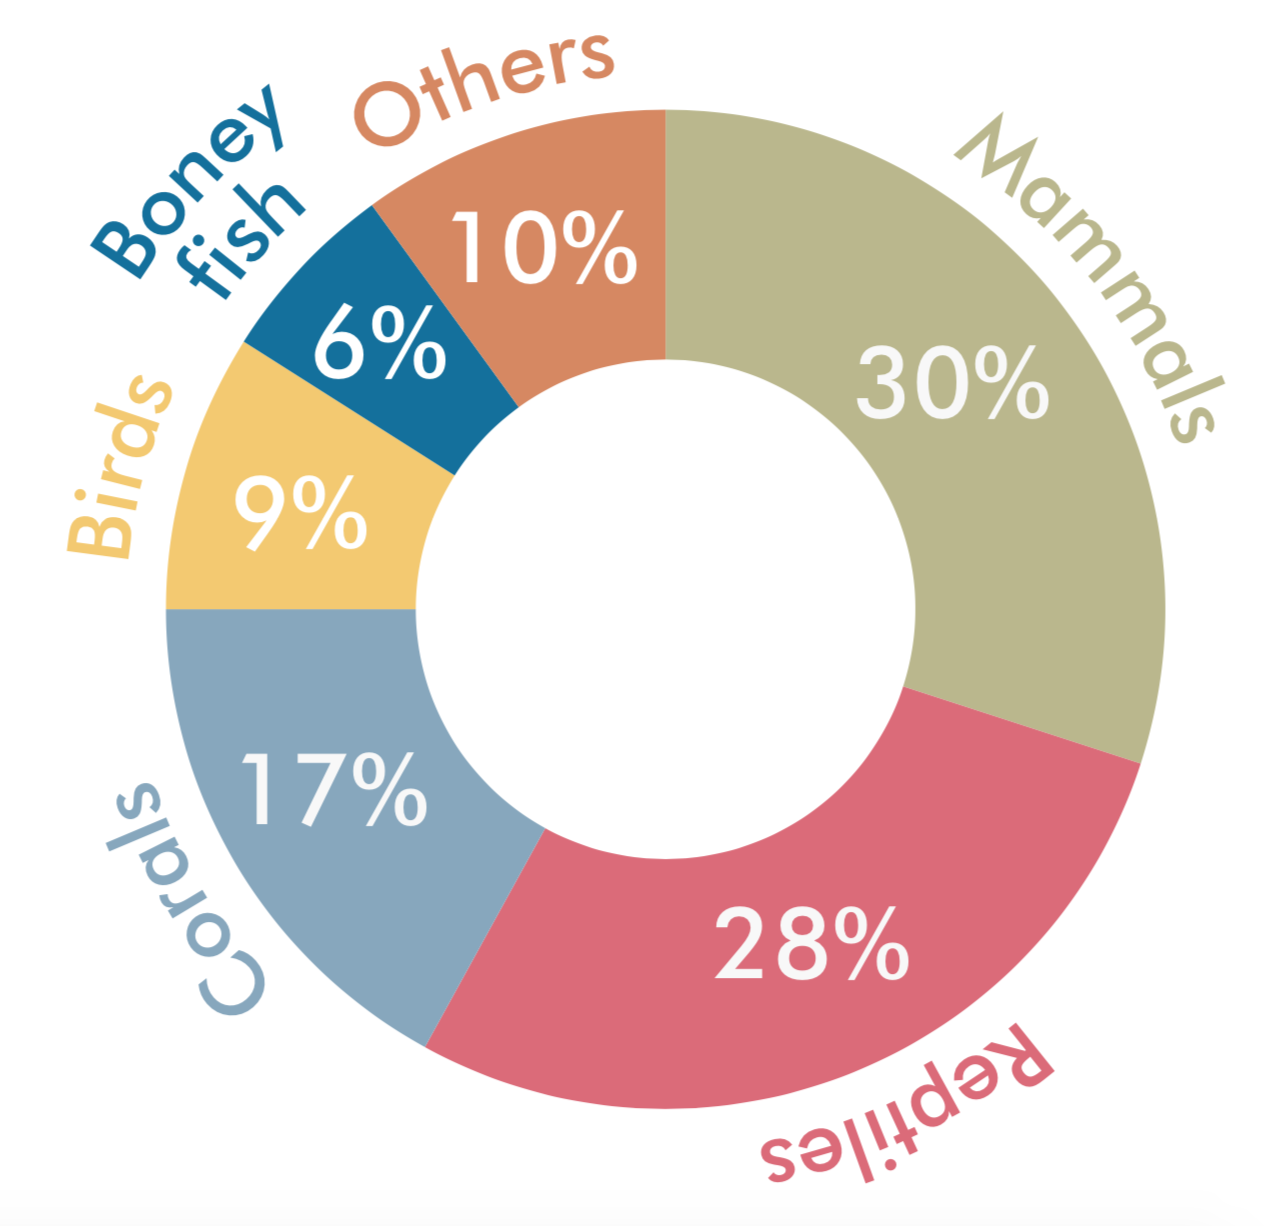
\includegraphics[width=0.5\textwidth]{figures/classes.png}\\
		\end{figure}
		\footnotesize{\emph{1999--2015 data on aggregated seizures*}}
	\end{center}
\end{frame}


%--------------------------%
% Generalities: Species II %
%--------------------------%	
\begin{frame}[t]
\frametitle{Generalities}
\framesubtitle{Species}
\vspace{0.25cm}

	\begin{reference}{4mm}{92mm}
		\rule{1.5cm}{0.25pt}\\
		UNODC (2016) World Wildlife Crime Report: Trafficking in protected species.
	\end{reference}

	International wildlife crime is committed for monetary gain
		\medskip
		\begin{itemize}
			\item Can quantify based on value of seizures
		\end{itemize}
		
		\begin{center}
			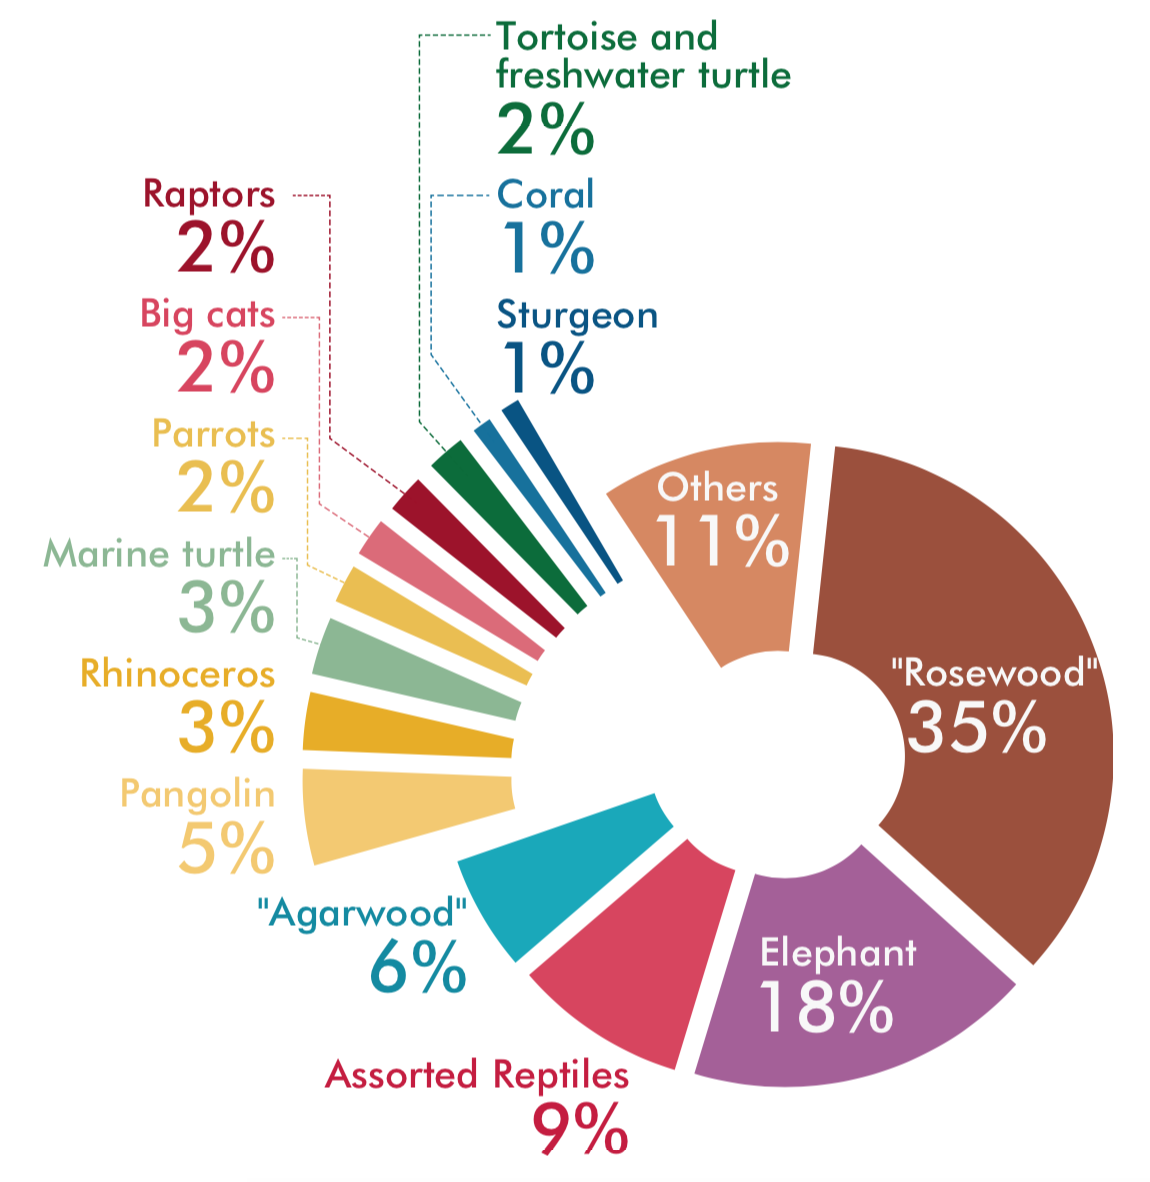
\includegraphics[width=0.5\textwidth]{figures/species_money.png}\\
			\vspace{0.1cm}
			\footnotesize{\emph{Data from seizures from 2005--2014}}
		\end{center}
\end{frame}


%---------------------------%
% Generalities: Species III %
%---------------------------%	
\begin{frame}[t]
\frametitle{Generalities}
\framesubtitle{Species}
\vspace{0.5cm}

	Could also quantify based on conservation impact:\\
	\medskip
		\begin{itemize}
			\item Number taken relative to total number alive\\
			\medskip
			\item 380 tiger skins collected from 2005--2014 worth only \$4 million, but only 3,000 tigers left!
		\end{itemize}
\end{frame}


%---------------------------%
% Generalities: Species IV  %
%---------------------------%	
\begin{frame}[t]
\frametitle{Generalities}
\framesubtitle{Species}
\vspace{0.5cm}

	Sometimes, multiple species are trafficked together\\
		\begin{itemize}
			\item Elephant ivory, rhino horn, pangolin scales\\
		\end{itemize}
	
	\bigskip	
	
	But most seizures are of a single species\\
		\begin{itemize}
			\item Suggesting that most international traffickers specialize in one species
		\end{itemize}
\end{frame}


%--------------------------%
% Generalities: Regions I  %
%--------------------------%	
\begin{frame}[t]
\frametitle{Generalities}
\framesubtitle{Countries/regions}
\vspace{0.25cm}

	\begin{reference}{4mm}{92mm}
		\rule{1.5cm}{0.25pt}\\
		UNODC (2016) World Wildlife Crime Report: Trafficking in protected species.
	\end{reference}

	Almost every country in the world is involved, with no single country being involved in $>15$\% of total seizures.
		\medskip
		\begin{itemize}
			\item However, clear patterns and roles for specific markets
		\end{itemize}
	
	\vspace{0.25cm}
	
	\begin{center}
		\begin{figure}
			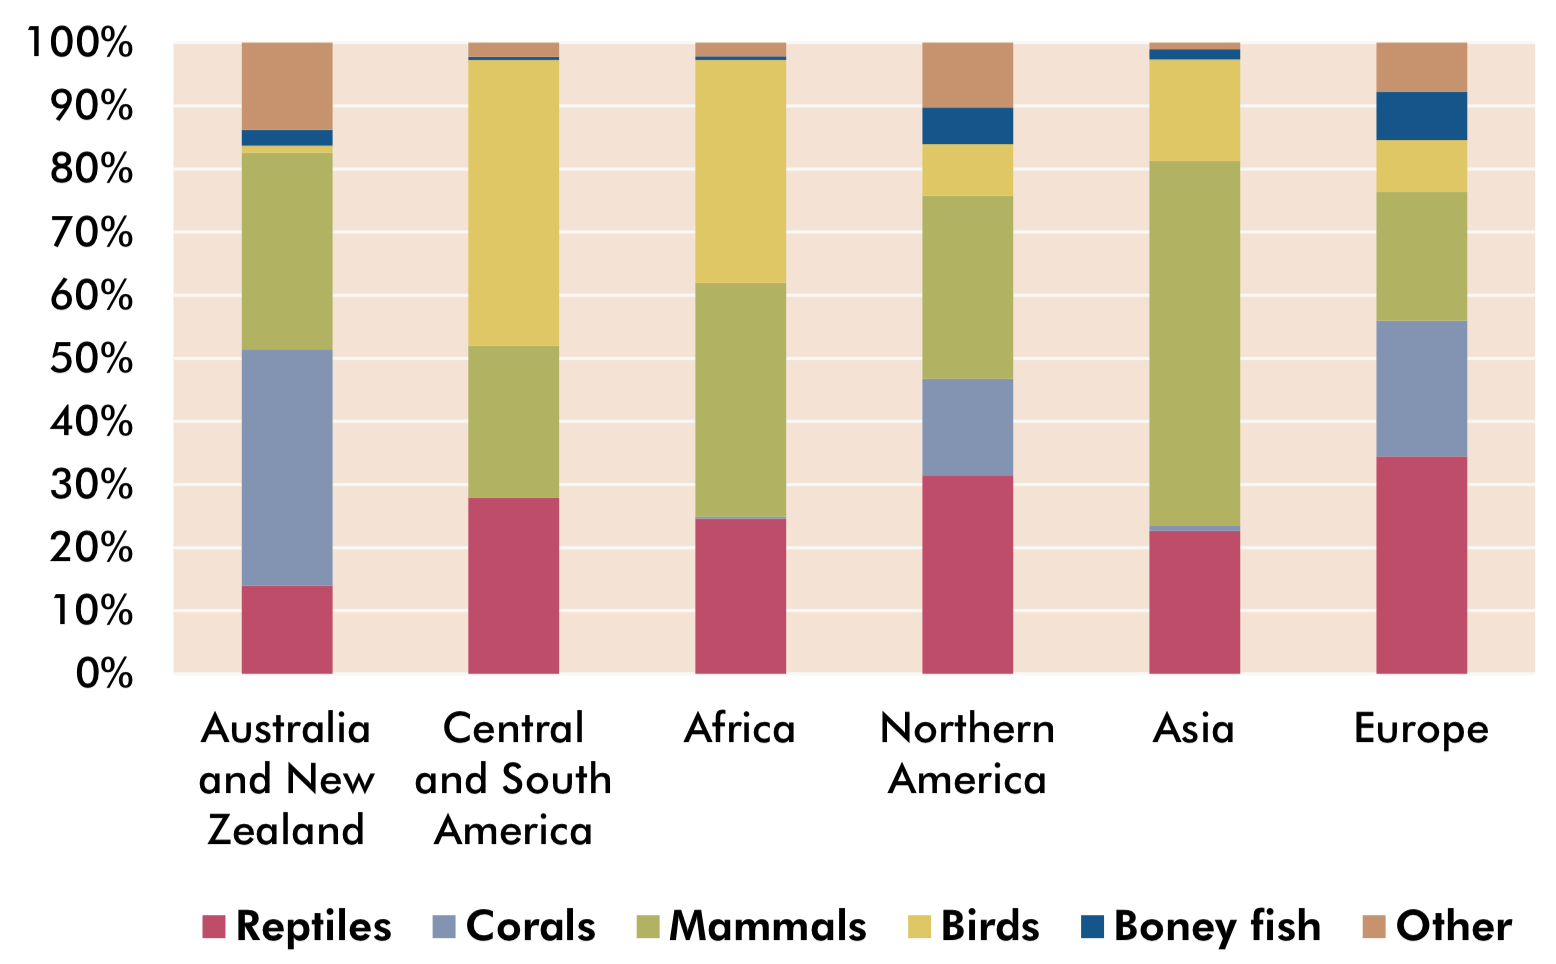
\includegraphics[width=0.7\textwidth]{figures/regions.png}\\
		\end{figure}
		\footnotesize{\emph{1999--2015 data on aggregated seizures by region}}
	\end{center}
\end{frame}


%--------------------------%
% Case Studies             %
%--------------------------%	
\begin{frame}[t]
\frametitle{Case Studies}
\vspace{0.5cm}

	Most \emph{international} wildlife forensics issues are related to \textbf{7} major markets:\\
	
		\begin{enumerate}
			\item Furniture
			\smallskip
			\item Art, d\'{e}cor, and jewelry
			\smallskip
			\item Fashion
			\smallskip
			\item Cosmetics \& perfume
			\smallskip
			\item Food, medicine, \& tonics
			\smallskip 
			\item Pets, zoos, \& breeding
			\smallskip
			\item Seafood
		\end{enumerate}
	
	
\end{frame}


%--------------------------------------------------%
% Case Study #1: Tropical Hardwood Furniture Trade %
%--------------------------------------------------%
\begin{frame}
	\begin{center}
		\Large{\textbf{\textcolor{myblue}{Market \#1: Furniture}}}\\ \normalsize{}
		
		\vspace{0.25cm}
		
		Rosewood logs for tropical hardwood furniture trade\\
		
		\vspace{1.0cm}
		
		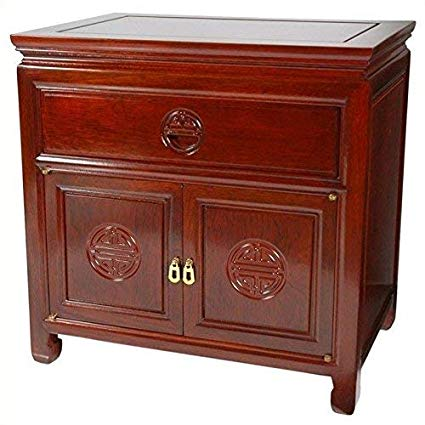
\includegraphics[width=0.3\textwidth]{figures/rosewood.jpg}
		
	\end{center}
\end{frame}


%---------------------------%
% Case Study #1             %
%---------------------------%
\begin{frame}[t]
\frametitle{Rosewood Trade}	
\vspace{0.5cm}

	\begin{reference}{4mm}{92mm}
		\rule{1.5cm}{0.25pt}\\
		1. UNODC (2016) World Wildlife Crime Report: Trafficking in protected species.
	\end{reference}

	Global production of furniture was valued at over \$400 billion in 2012$^1$\\
		\medskip
		\begin{itemize}
			\item Tropical hardwood furniture production was valued at $\sim$\$65 billion\\
				\smallskip
				\begin{itemize}
					\item 39\% of wooden furniture production
					\smallskip
					\item 16\% of total furniture production
				\end{itemize}
		\end{itemize}
	
	\begin{tikzpicture}[overlay]
		\node at (9,-1) (graph) {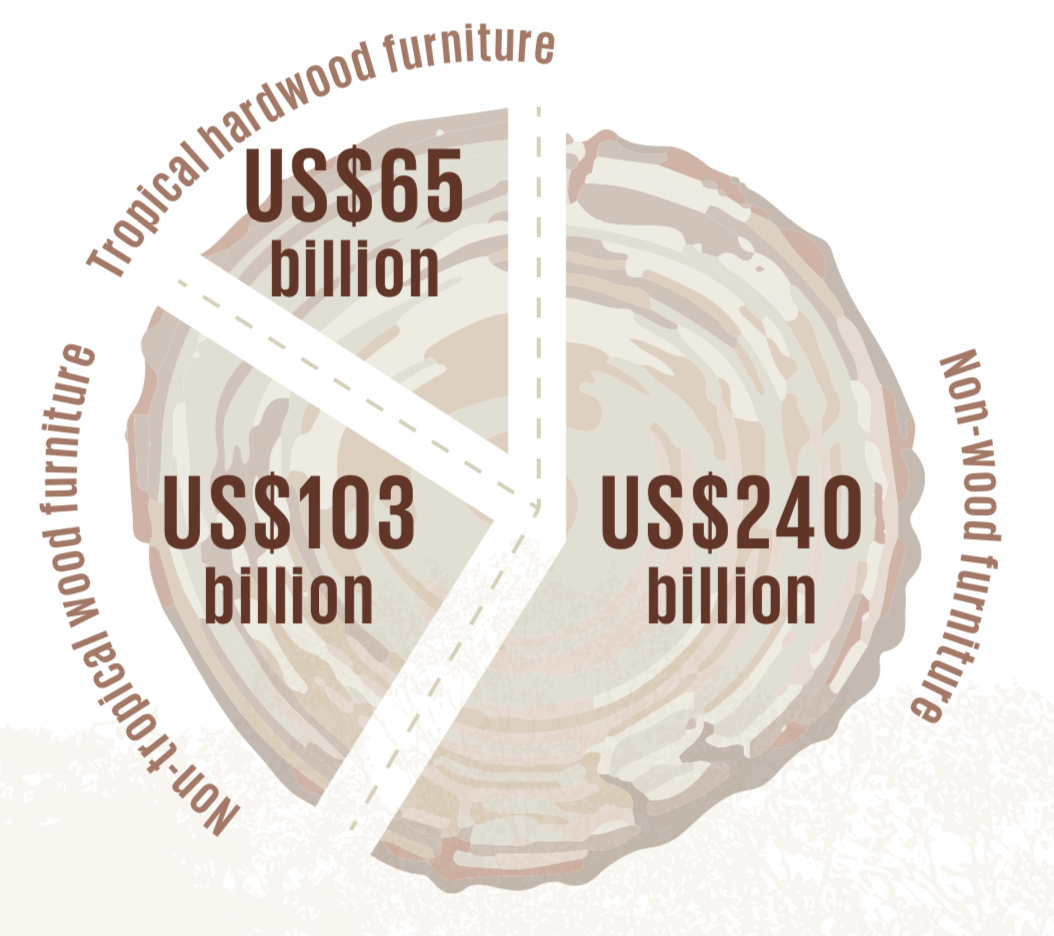
\includegraphics[width=0.45\textwidth]{figures/woodpie1.png}};
	\end{tikzpicture}	
\end{frame}


%---------------------------%
% Case Study #1             %
%---------------------------%
\begin{frame}[t]
\frametitle{Rosewood Trade}	
\vspace{0.5cm}

	Perhaps the most destructive wildlife trade, because it represents the destruction of habitats in addition to the exploitation of the traded species themselves
	
	\vspace{0.5cm}
	
	\begin{center}
		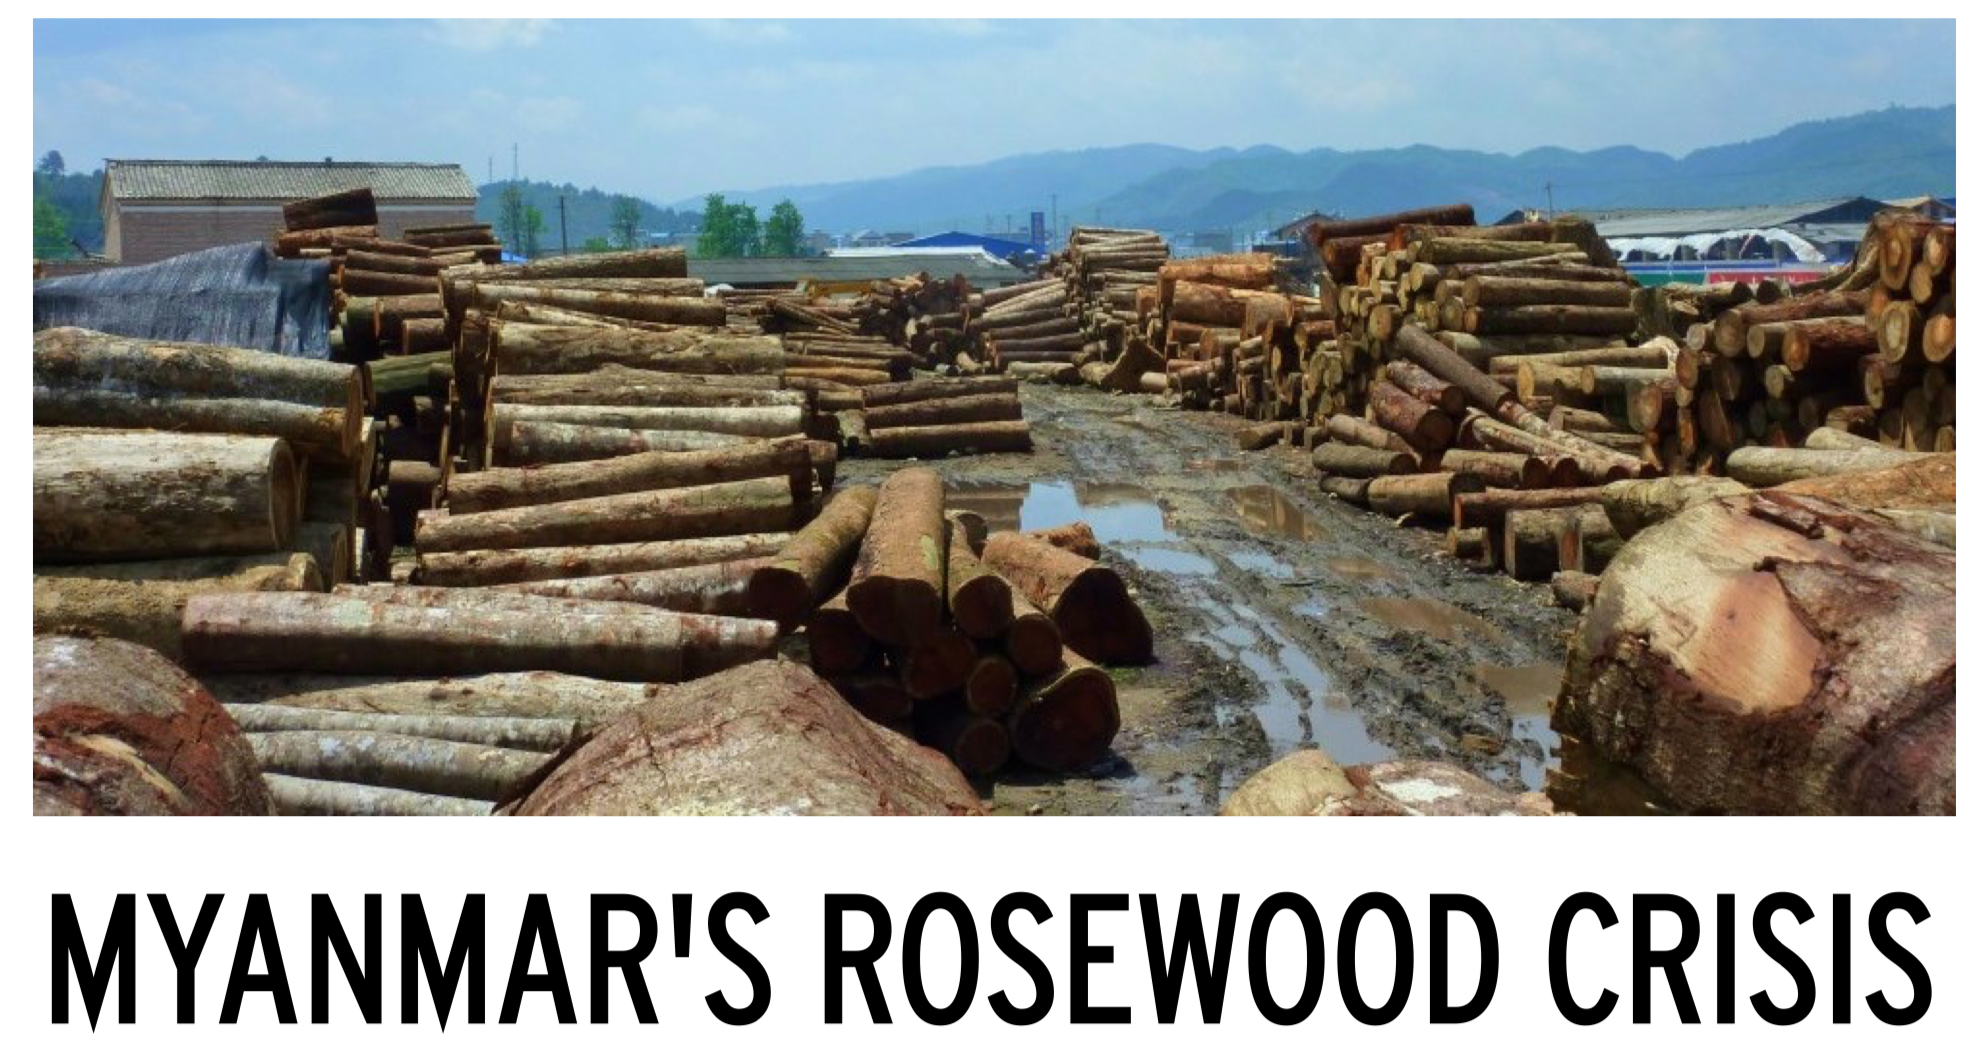
\includegraphics[width=0.75\textwidth]{figures/forest.png}
	\end{center}
\end{frame}


%---------------------------%
% Case Study #1             %
%---------------------------%
\begin{frame}[t]
\frametitle{Rosewood Trade}	
\vspace{1.0cm}

	\begin{block}{Rosewood}
		An imprecise term associated with a wide range of topical hardwoods that are richly hued and often fragrant.
	\end{block}	
\end{frame}


%----------------------------%
%  Case Study #1             %
%----------------------------%
\begin{frame}[t]
\frametitle{Rosewood Trade}
\vspace{0.5cm}

	Genus \emph{Dalbergia}\\
	
	\vspace{0.5cm}
	
	\begin{columns}
		\begin{column}{0.5\textwidth}
			\begin{center}
				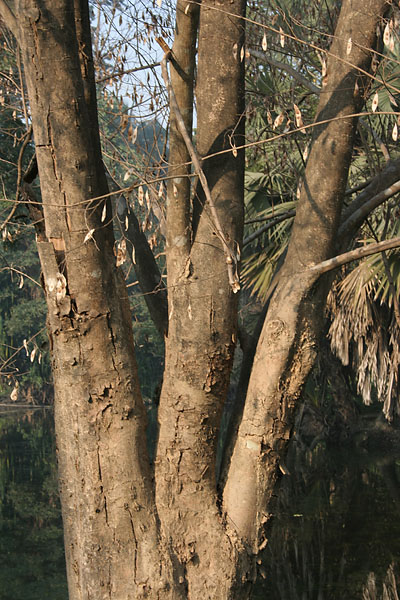
\includegraphics[width=0.6\textwidth]{figures/dalbergia.jpg}
			\end{center}
		\end{column}
		
		\begin{column}{0.5\textwidth}
			\begin{center}
				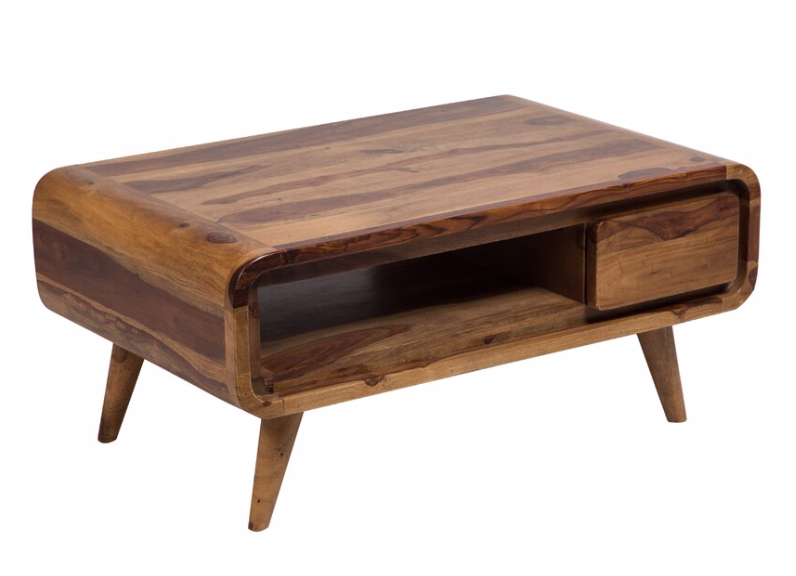
\includegraphics[width=1.0\textwidth]{figures/dalbergia2.png}
			\end{center}
		\end{column}
	\end{columns}
\end{frame}


%----------------------------%
%  Case Study #1             %
%----------------------------%
\begin{frame}[t]
\frametitle{Rosewood Trade}
\vspace{0.5cm}

	Genus \emph{Pterocarpus}\\
	
	\vspace{0.5cm}
	
	\begin{columns}
		\begin{column}{0.5\textwidth}
			\begin{center}
				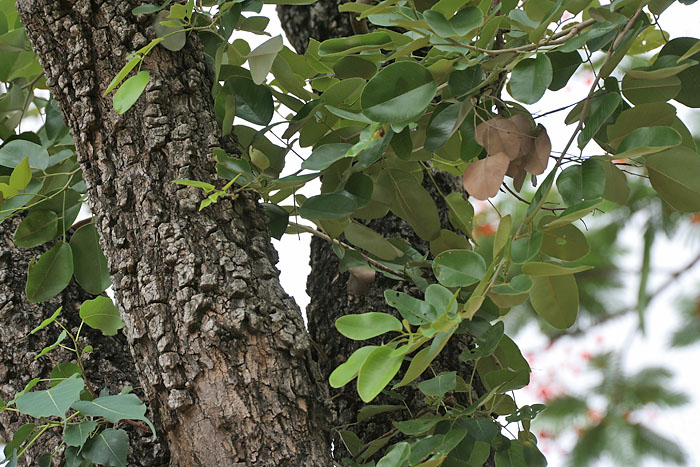
\includegraphics[width=0.8\textwidth]{figures/pterocarpus.jpg}
			\end{center}
		\end{column}
		
		\begin{column}{0.5\textwidth}
			\begin{center}
				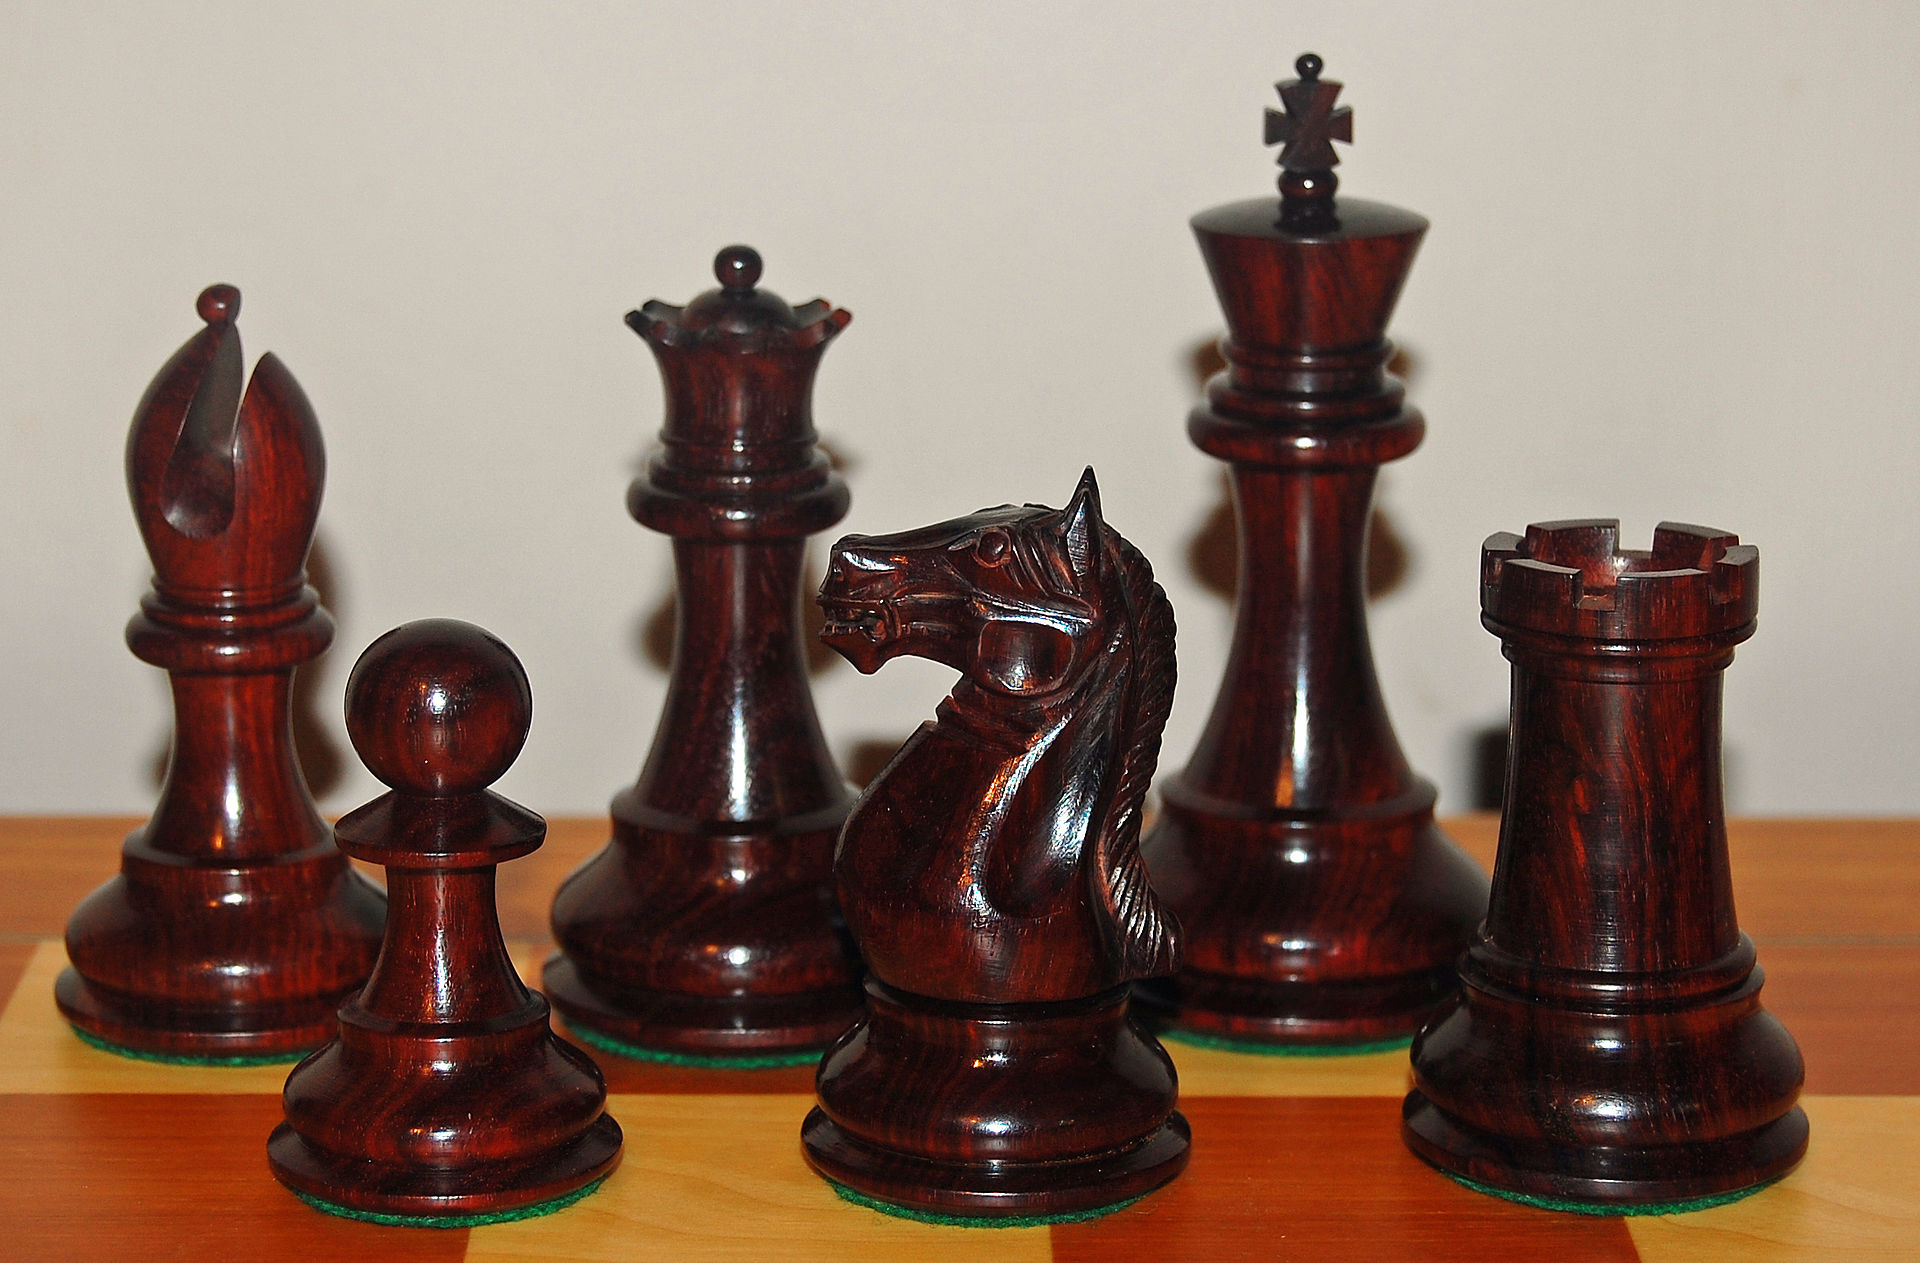
\includegraphics[width=0.8\textwidth]{figures/pterocarpus2.jpg}
			\end{center}
		\end{column}
	\end{columns}
\end{frame}


%----------------------------%
%  Case Study #1             %
%----------------------------%
\begin{frame}[t]
\frametitle{Rosewood Trade}
\vspace{0.25cm}

	Many species of each, some of which are protected, some are not\\
		\begin{itemize}
			\item Tracking particular species extremely difficult, particularly when processed
		\end{itemize}
		
	\vspace{0.25cm}

	\begin{center}
		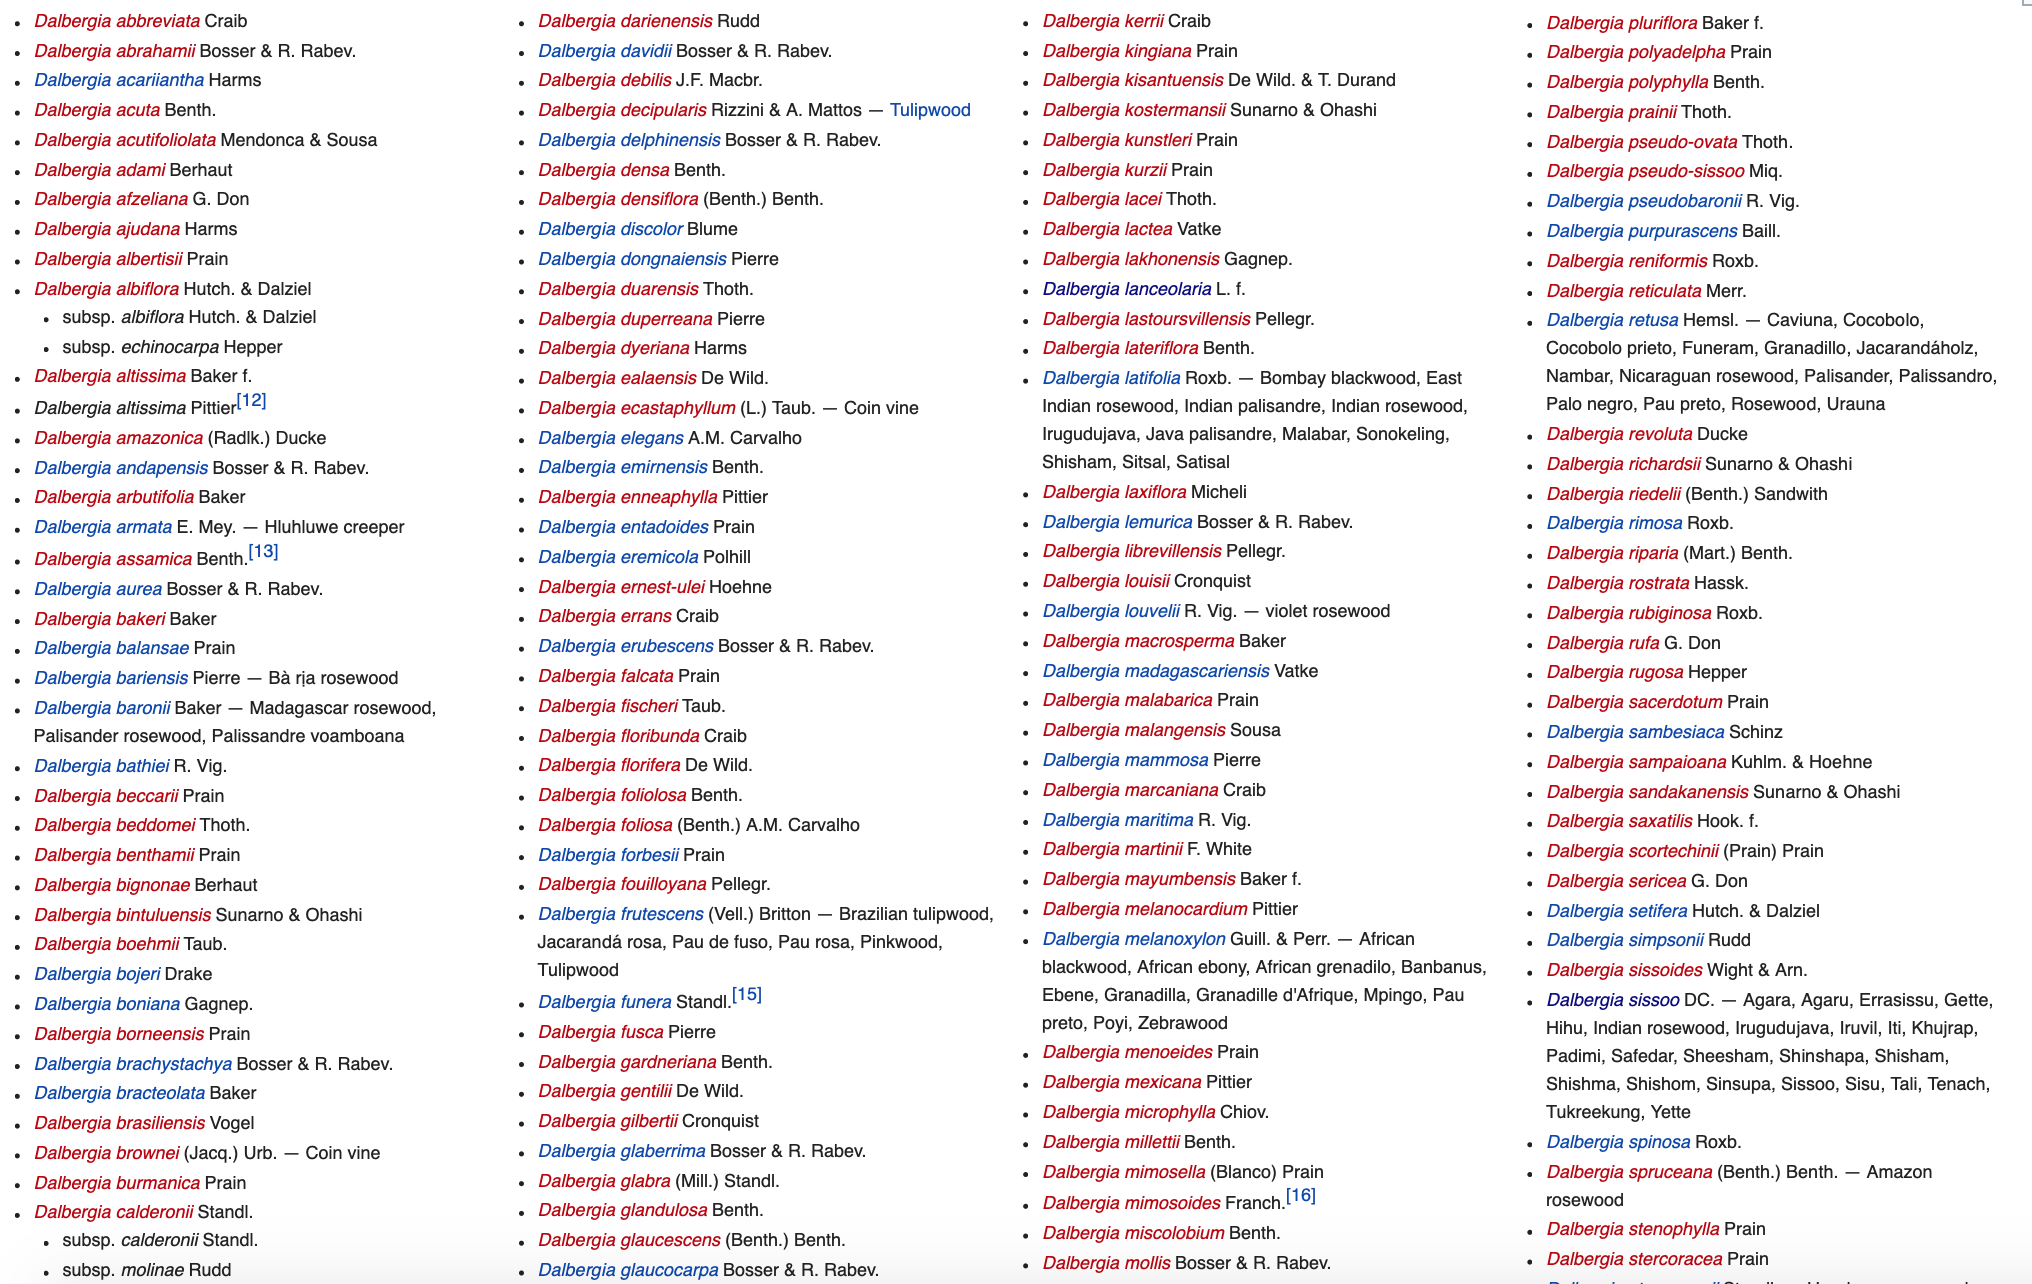
\includegraphics[width=0.7\textwidth]{figures/Dspecies.png}
	\end{center}
\end{frame}


%----------------------------%
%  Case Study #1             %
%----------------------------%
\begin{frame}[t]
\frametitle{Rosewood Trade}
\vspace{0.25cm}

	\begin{reference}{4mm}{92mm}
		\rule{1.5cm}{0.25pt}\\
		UNODC (2016) World Wildlife Crime Report: Trafficking in protected species.
	\end{reference}
	
	Major \textcolor{myblue}{sources} are countries in southeast Asia and the Pacific, and China is by far the greatest \textcolor{myblue}{consumer}\\
	
	\vspace{0.5cm}
	
	\begin{center}
		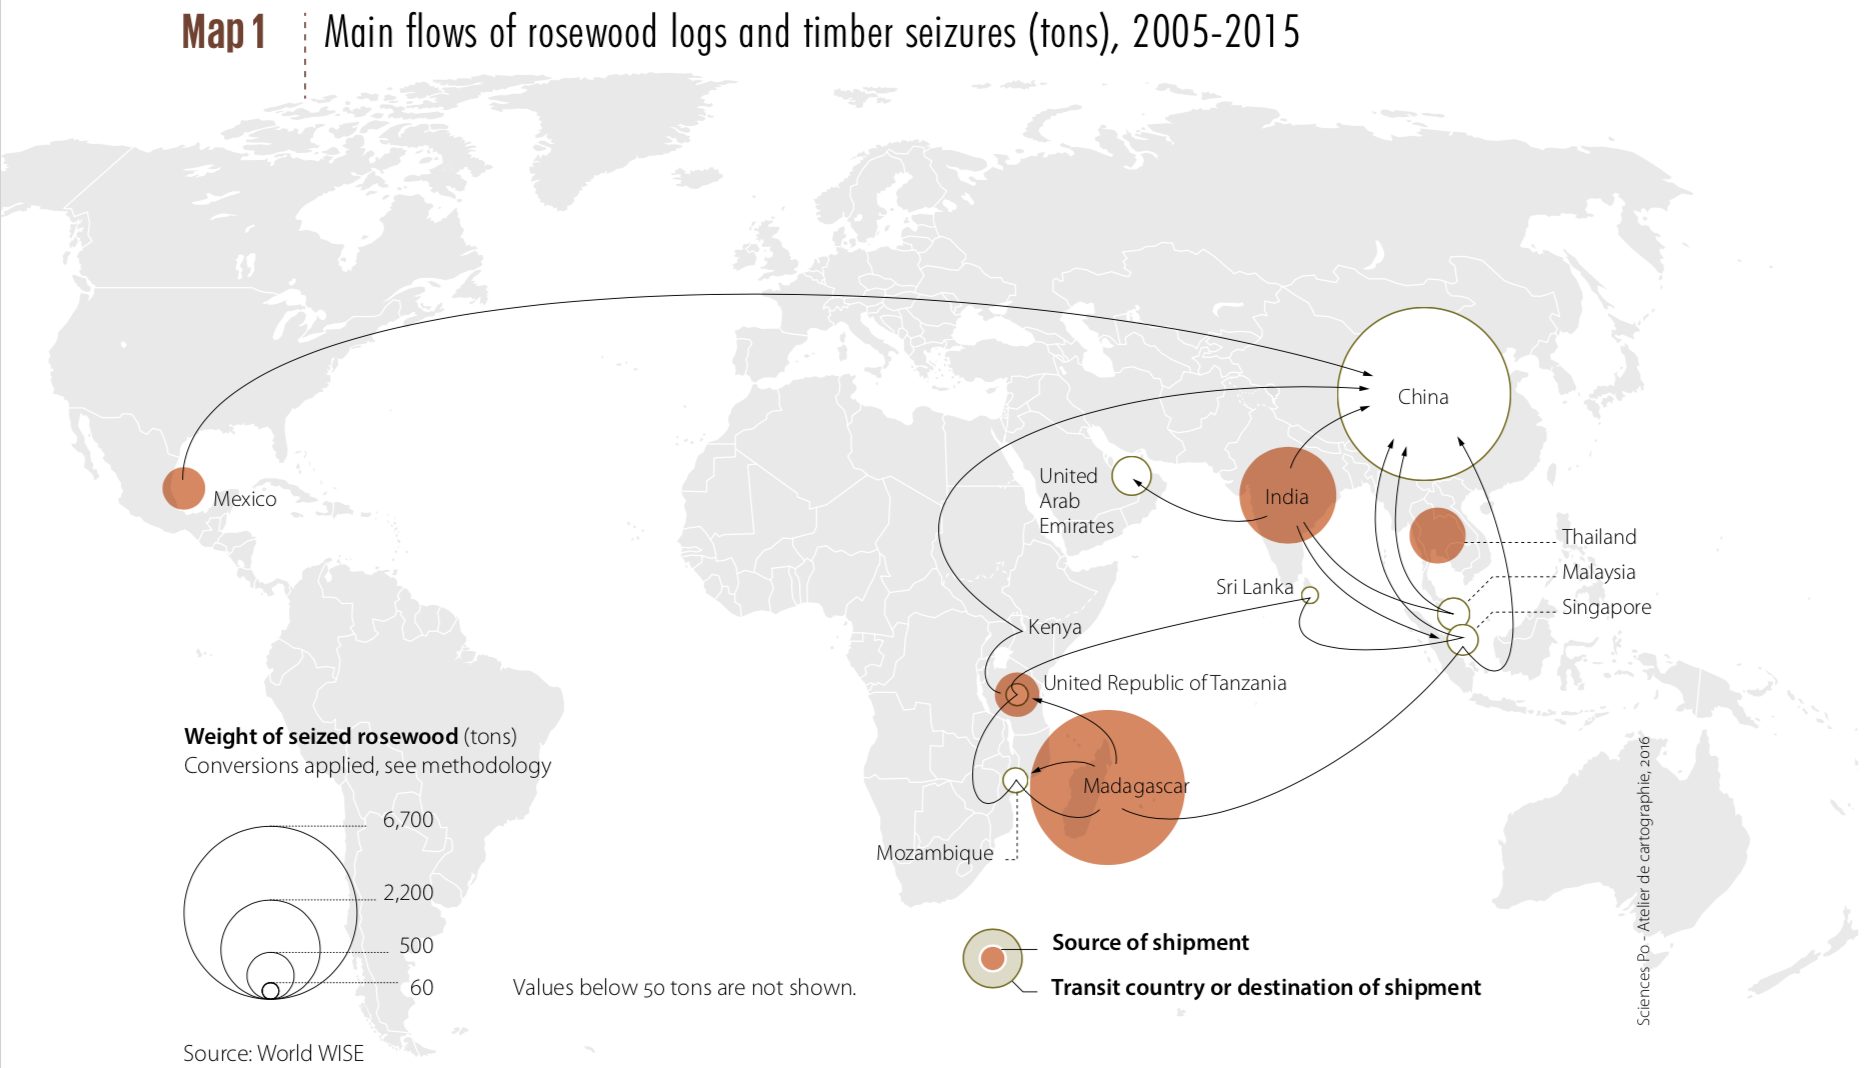
\includegraphics[width=0.9\textwidth]{figures/map1.png}
	\end{center}
\end{frame}


%----------------------------%
%  Case Study #1             %
%----------------------------%
\begin{frame}[t]
\frametitle{Rosewood Trade}
\vspace{0.5cm}

	\begin{reference}{4mm}{92mm}
		\rule{1.5cm}{0.25pt}\\
		*Unless it is an internationally protected species
	\end{reference}
	
	
	Threatened with extensive deforestation, some source countries have developed log export bans and/or protection for specific species\\
	
	\vspace{0.25cm}
	
	\begin{itemize}
		\item Once illegally exported (and out of that jurisdiction), not illegal to import into other countries*
		\medskip
		\item Consumers may legally purchase products, even though original harvesting was illegal
	\end{itemize}
\end{frame}


%----------------------------%
%  Case Study #1             %
%----------------------------%
\begin{frame}[t]
\frametitle{Rosewood Trade}
\vspace{0.25cm}

	Where is this wood originally from? What species is it? Is this from a legal source?\\
	
	\vspace{0.25cm}
	
	\begin{center}
		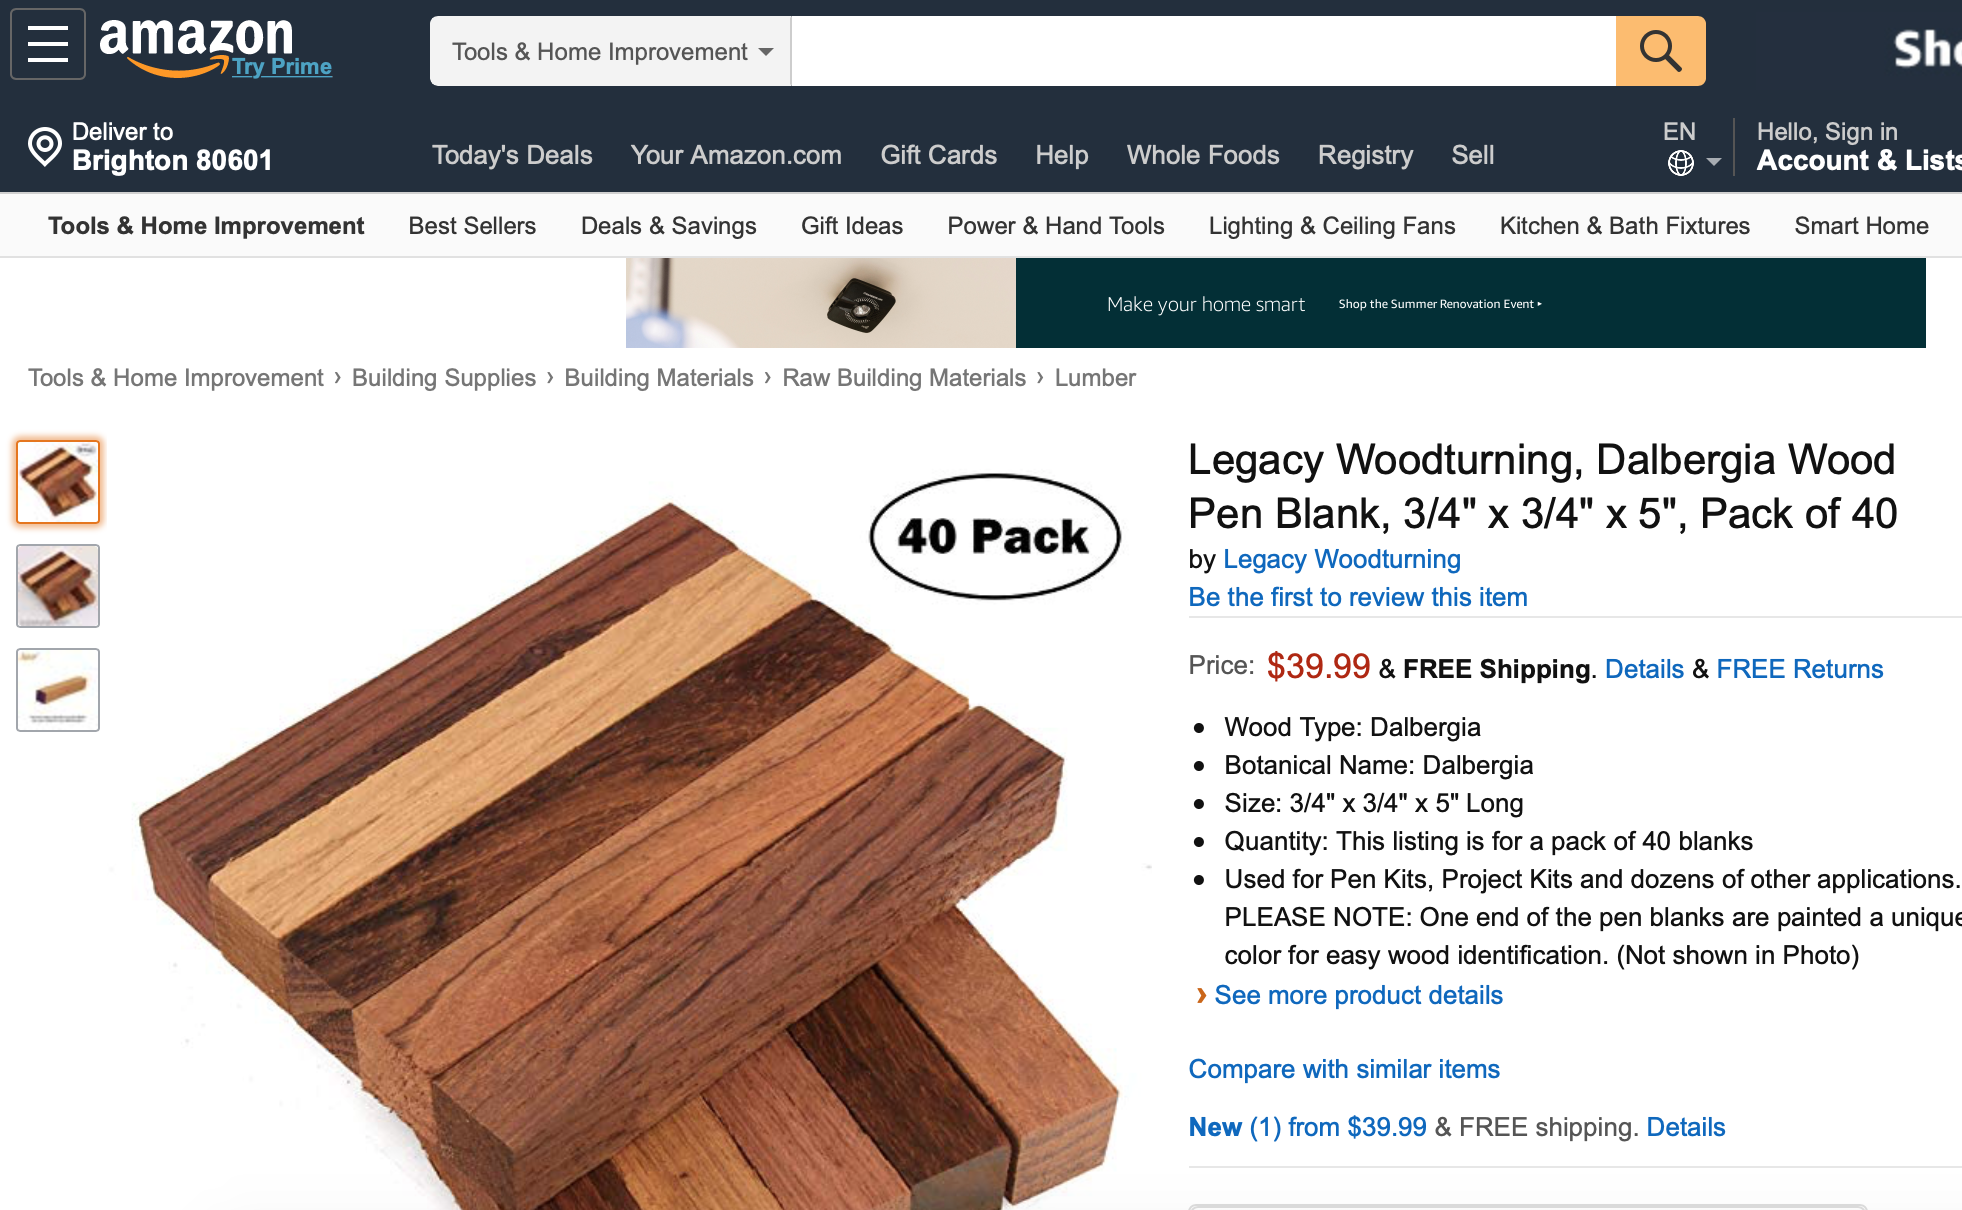
\includegraphics[width=0.65\textwidth]{figures/amazon.png}
	\end{center} 
\end{frame}


%----------------------------%
%  Case Study #1             %
%----------------------------%
\begin{frame}[t]
\frametitle{Rosewood Trade}
\vspace{0.5cm}

	In countries with export bans, some may still be legal\\
		\medskip
		\begin{itemize}
			\item Trees felled \emph{before} ban was in place
			\medskip
			\item Trees felled for other purposes (construction, development, etc.)
		\end{itemize}
		\bigskip
	
	Through these loopholes, illegally harvested wood can make it into the legal market, even within the source country	
\end{frame}


%---------------------------------------%
% Case Study #2: Art, decor, jewelry    %
%---------------------------------------%
\begin{frame}
	\begin{center}
		\Large{\textbf{\textcolor{myblue}{Market \#2:\\ Art, D\'{e}cor, \& Jewelry:}}}\normalsize{}\\ 
		
		\vspace{0.25cm}
		
		The African Elephant Ivory Trade\\
		
		\vspace{1.0cm}
		
		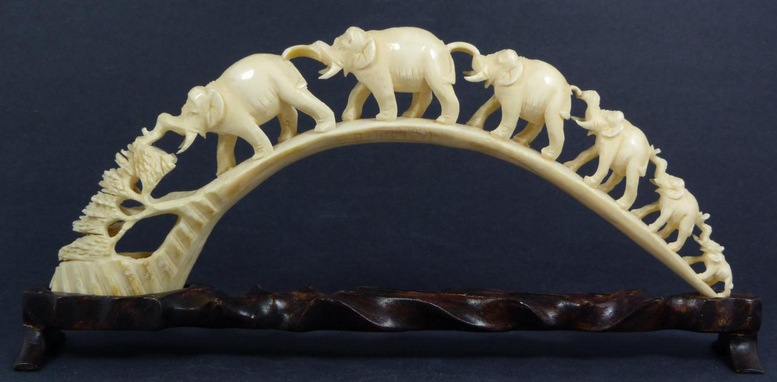
\includegraphics[width=0.6\textwidth]{figures/ivory.png}
		
	\end{center}
\end{frame}


%---------------------------------------%
% Case Study #2: Art, decor, jewelry    %
%---------------------------------------%
\begin{frame}[t]
\frametitle{Elephant Ivory Trade}
\vspace{0.5cm}

	Some products---particularly in the art, d\'{e}core, and jewelry market---have attained a value detached from any practical uses they once had
	
	\vspace{0.5cm}
	
	To achieve this, usually must combine:\\
		\medskip
		\begin{enumerate}
			\item Traditionally recognized as precious
			\medskip
			\item Supply is limited
		\end{enumerate}
\end{frame}


%---------------------------------------%
% Case Study #2: Art, decor, jewelry    %
%---------------------------------------%
\begin{frame}[t]
\frametitle{Elephant Ivory Trade}
\vspace{0.5cm}

	These items serve many purposes apart from their original value:\\
		\medskip
		\begin{enumerate}
			\item Value stores (maintain value regardless of financial market)
			\medskip
			\item Exhibition of cultural credentials (in areas where traditional ways are valued)
			\medskip
			\item Demonstrate political connections (in areas where they are under strict control)
		\end{enumerate}
\end{frame}


%---------------------------------------%
% Case Study #2: Art, decor, jewelry    %
%---------------------------------------%
\begin{frame}[t]
\frametitle{Elephant Ivory Trade}
\vspace{0.5cm}

	Elephant ivory ticks all of these boxes:\\
	\medskip
		\begin{itemize}
			\item Traditionally a precious commodity, from which ``high art'' was made
			\medskip
			\item With growing market restrictions, exclusivity has been enhanced\\
		\end{itemize}
	
	\vspace{0.5cm}
	
	Ivory has thus become extremely valuable in a world of dramatic economic changes\\
	
	\vspace{0.5cm}
	
	One strange thing about ivory trade, supply far outweighs market demand, suggesting use as ``insurance''
\end{frame}


%---------------------------------------%
% Case Study #2: Art, decor, jewelry    %
%---------------------------------------%
\begin{frame}[t]
\frametitle{Elephant Ivory Trade}
\vspace{0.25cm}

	\begin{reference}{4mm}{92mm}
		\rule{1.5cm}{0.25pt}\\
		1. UNODC (2016) World Wildlife Crime Report: Trafficking in protected species.
	\end{reference}

	Are roughly 500,000 elephants left in Africa (different species)$^{1}$\\
	
	\vspace{0.25cm}
	
	Spread unevenly across 37 countries\\
		\medskip
		\begin{itemize}
			\item $>$60\% in Botswana, Zimbabwe, \& United Republic of Tanzania\\
		\end{itemize}
	
	\vspace{0.25cm}
	
	\begin{columns}
		\begin{column}{0.5\textwidth}
			\begin{center}
				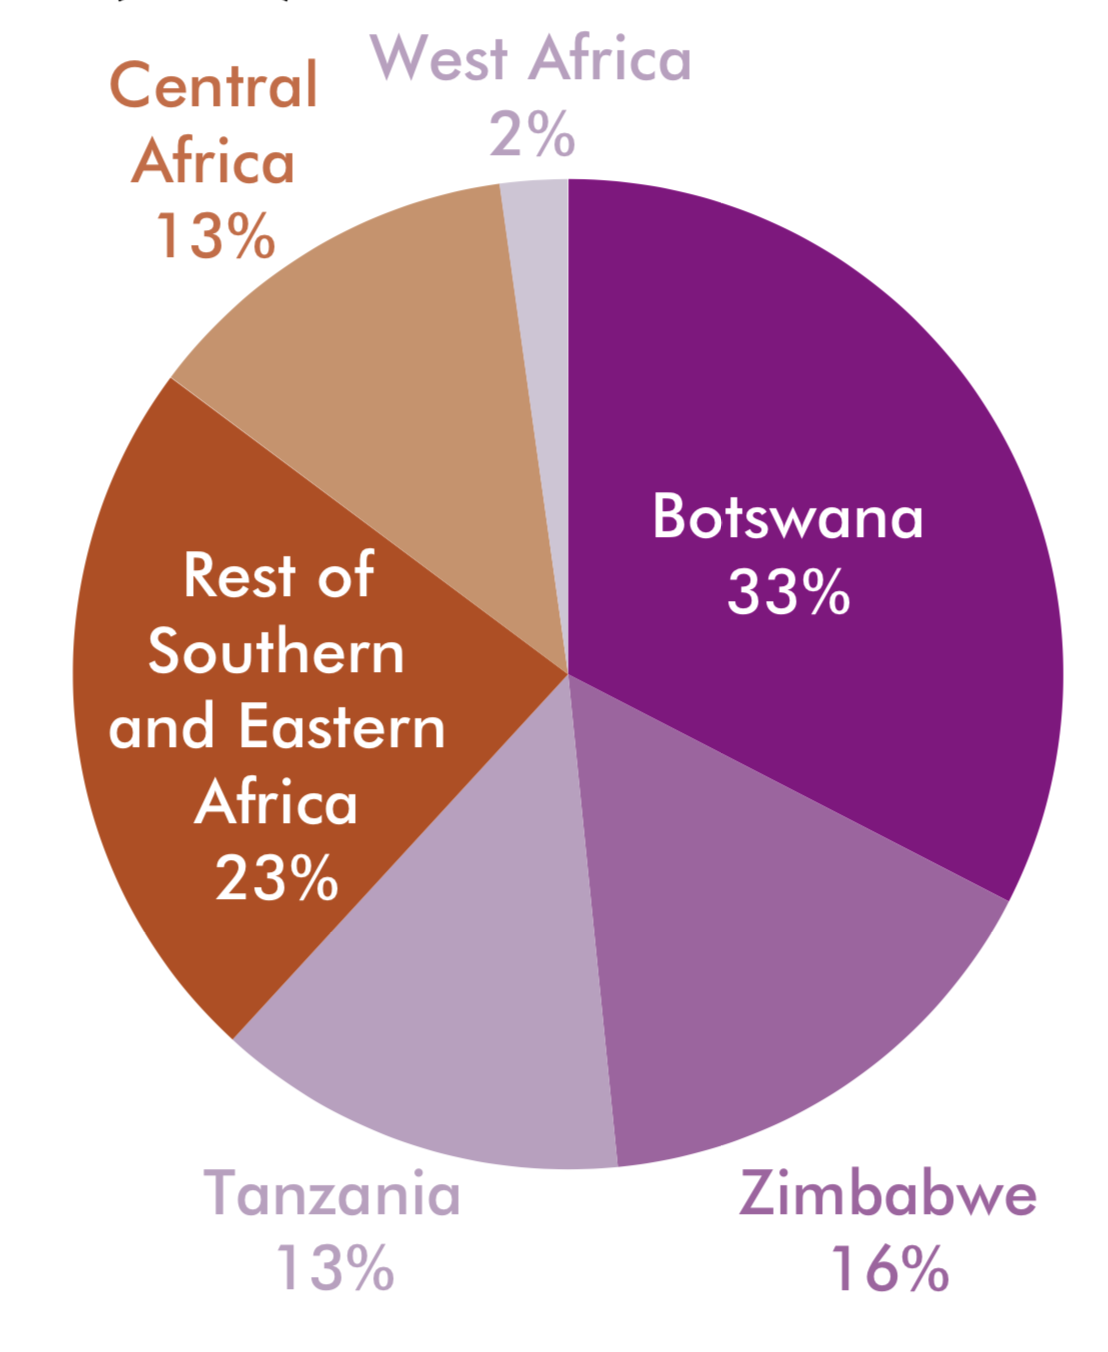
\includegraphics[width=0.8\textwidth]{figures/eCountries1.png}	
			\end{center}
		\end{column}
		
		\begin{column}{0.5\textwidth}
			\begin{center}
				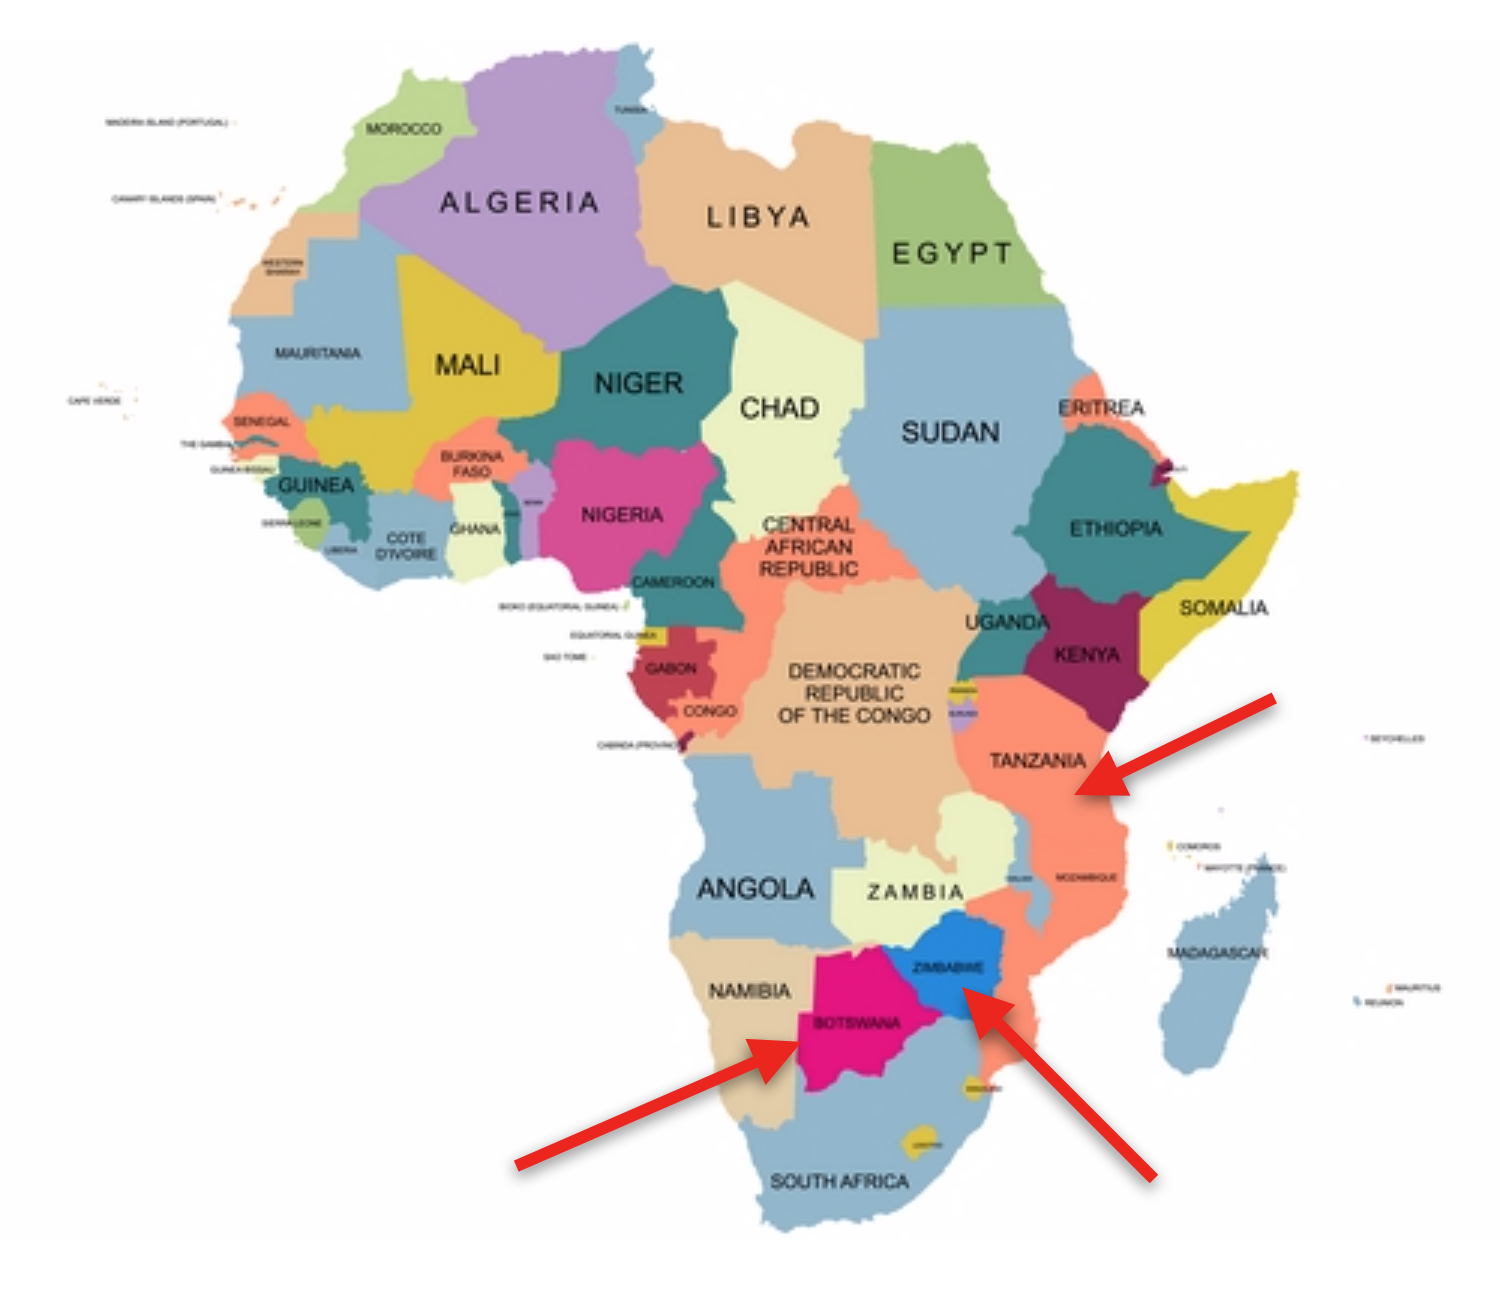
\includegraphics[width=1.1\textwidth]{figures/eCountries2.png}	
			\end{center}
		\end{column}
	\end{columns}	
\end{frame}


%---------------------------------------%
% Case Study #2: Art, decor, jewelry    %
%---------------------------------------%
\begin{frame}[t]
\frametitle{Elephant Ivory Trade}
\vspace{0.5cm}

	\begin{reference}{4mm}{92mm}
		\rule{1.5cm}{0.25pt}\\
		UNODC (2016) World Wildlife Crime Report: Trafficking in protected species.
	\end{reference}
	
	China is the largest importer, but other countries in southeast Asia big too\\
	
	\vspace{0.25cm}
	
	\begin{center}
		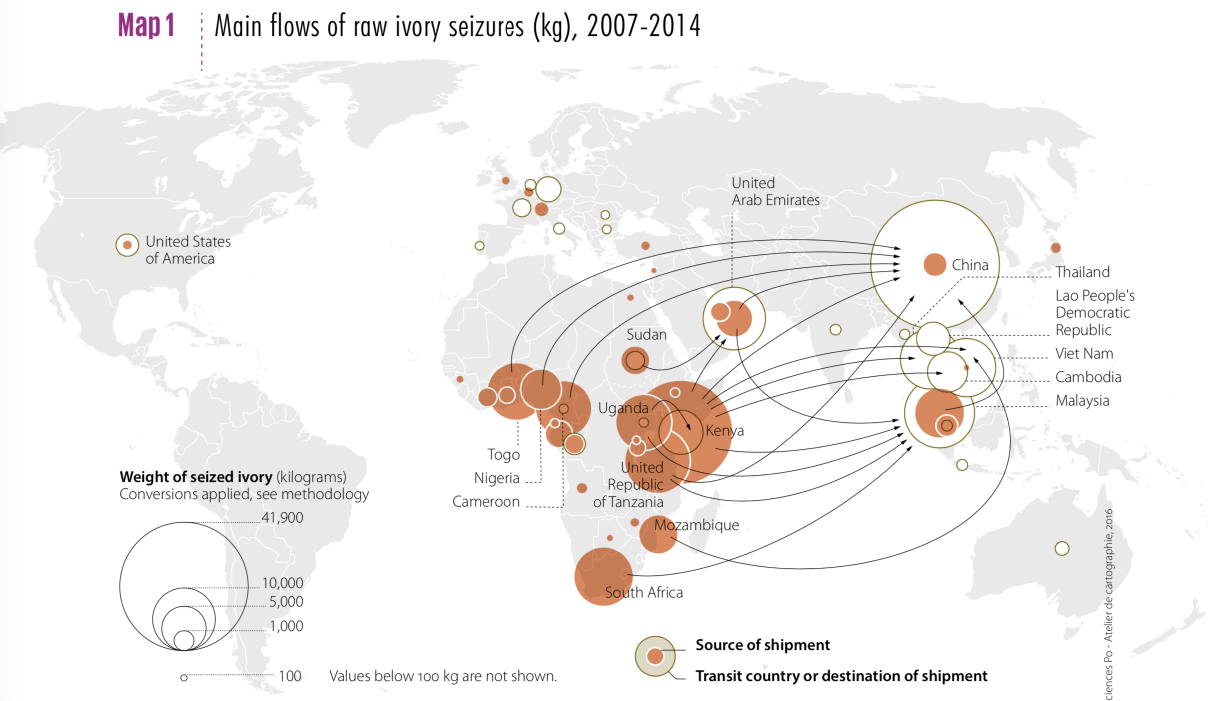
\includegraphics[width=0.9\textwidth]{figures/map2.png}
	\end{center}
\end{frame}


%---------------------------------------%
% Case Study #2: Art, decor, jewelry    %
%---------------------------------------%
\begin{frame}[t]
\frametitle{Elephant Ivory Trade}
\vspace{0.5cm}

	\begin{reference}{4mm}{92mm}
		\rule{1.5cm}{0.25pt}\\
		UNODC (2016) World Wildlife Crime Report: Trafficking in protected species.
	\end{reference}
	
	Over 20,000 elephants are poached each year\\
		\medskip
		\begin{itemize}
			\item Some populations declining
			\medskip
		\end{itemize}
	
	\vspace{0.25cm}
	
	\begin{center}
		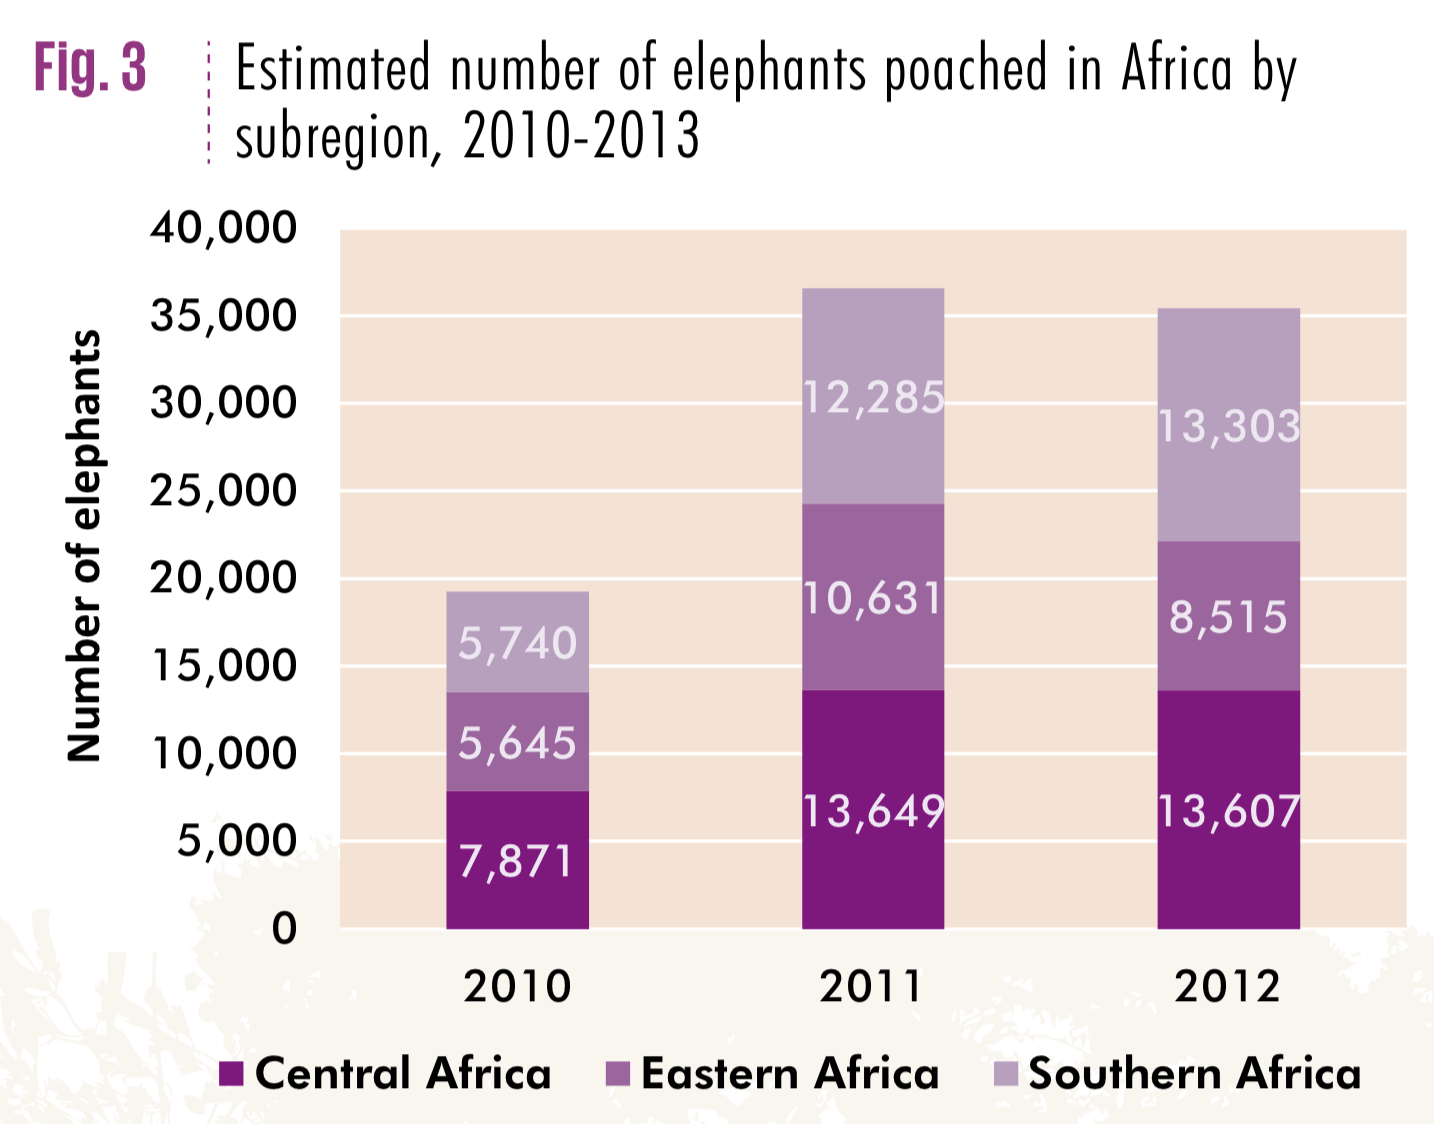
\includegraphics[width=0.65\textwidth]{figures/ePoaching1.png}
	\end{center}
\end{frame}


%---------------------------------------%
% Case Study #2: Art, decor, jewelry    %
%---------------------------------------%
\begin{frame}[t]
\frametitle{Elephant Ivory Trade}
\vspace{0.5cm}

	\begin{reference}{4mm}{92mm}
		\rule{1.5cm}{0.25pt}\\
		1. UNODC (2016) World Wildlife Crime Report: Trafficking in protected species.
	\end{reference}
	
	United Republic of Tanzania seems to be an important target\\
	\medskip
		\begin{itemize}
			\item Population declined by $>$50\% between 2007 and 2013$^{1}$
			\medskip
			\item Interestingly, DNA data show primarily from two reserves:
				\begin{enumerate}
					\item Selous
					\item Ruaha
				\end{enumerate}
		\end{itemize}
	
	\begin{center}
		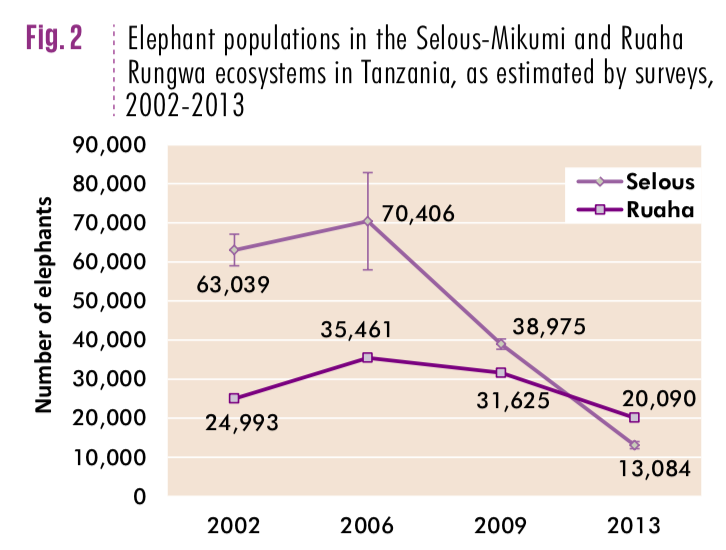
\includegraphics[width=0.5\textwidth]{figures/ePoaching2.png}
	\end{center}	
\end{frame}


%---------------------------------------%
% Case Study #2: Art, decor, jewelry    %
%---------------------------------------%
\begin{frame}[t]
\frametitle{Elephant Ivory Trade}
\vspace{0.5cm}

	Poachers involved represent a range of people (opportunists--dedicated hunters)\\
	\medskip
		\begin{itemize}
			\item Large \# from reserves suggests a high degree of corruption\\
			\medskip
			\item Data suggest link between poaching and insurgent groups not as strong as often portrayed\\
		\end{itemize}
	
	\begin{center}
		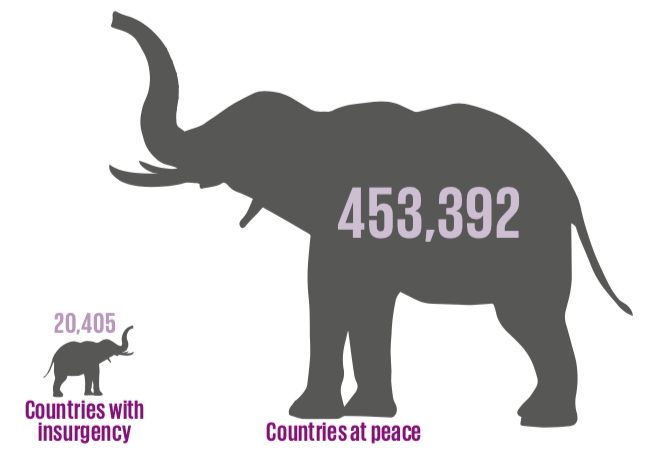
\includegraphics[width=0.6\textwidth]{figures/ePoaching3.png}
	\end{center}		

\end{frame}


%---------------------------------------%
% Case Study #2: Art, decor, jewelry    %
%---------------------------------------%
\begin{frame}
\frametitle{Elephant Ivory Trade}

	\begin{center}
		\href{https://www.youtube.com/watch?time_continue=185&v=5gQujyNDp98}{\Large{\textbf{Video}}}	
	\end{center}	

\end{frame}


%---------------------------------------%
% Case Study #2: Art, decor, jewelry    %
%---------------------------------------%
\begin{frame}[t]
\frametitle{Elephant Ivory Trade}
\vspace{0.5cm}

	Problems (other than the obvious):\\
	\medskip
		\begin{enumerate}
			\item Many countries have stockpiles, the trade of which may be legal
				\begin{itemize}
					\item Pre-regulation purchases
					\item Natural mortalities
					\item Contraband seizure
				\end{itemize}
			\medskip
			\item Domestic trade legal in many countries
				\begin{itemize}
					\item Once inside such a country, trade is legal\\
				\end{itemize}	
			\medskip
			\item Exporting countries/seizures are often not the country of origin (``staging areas'')
		\end{enumerate}

	\medskip
	
	Represent loopholes through which illegal ivory can be integrated into the legal trade
\end{frame}


%---------------------------------------%
% Case Study #3: Fashion                %
%---------------------------------------%
\begin{frame}
	\begin{center}
		\Large{\textbf{\textcolor{myblue}{Market \#3:\\ Fashion:}}}\normalsize{}\\ 
		
		\vspace{0.25cm}
		
		Reptile Skins\\
		
		\vspace{1.0cm}
		
		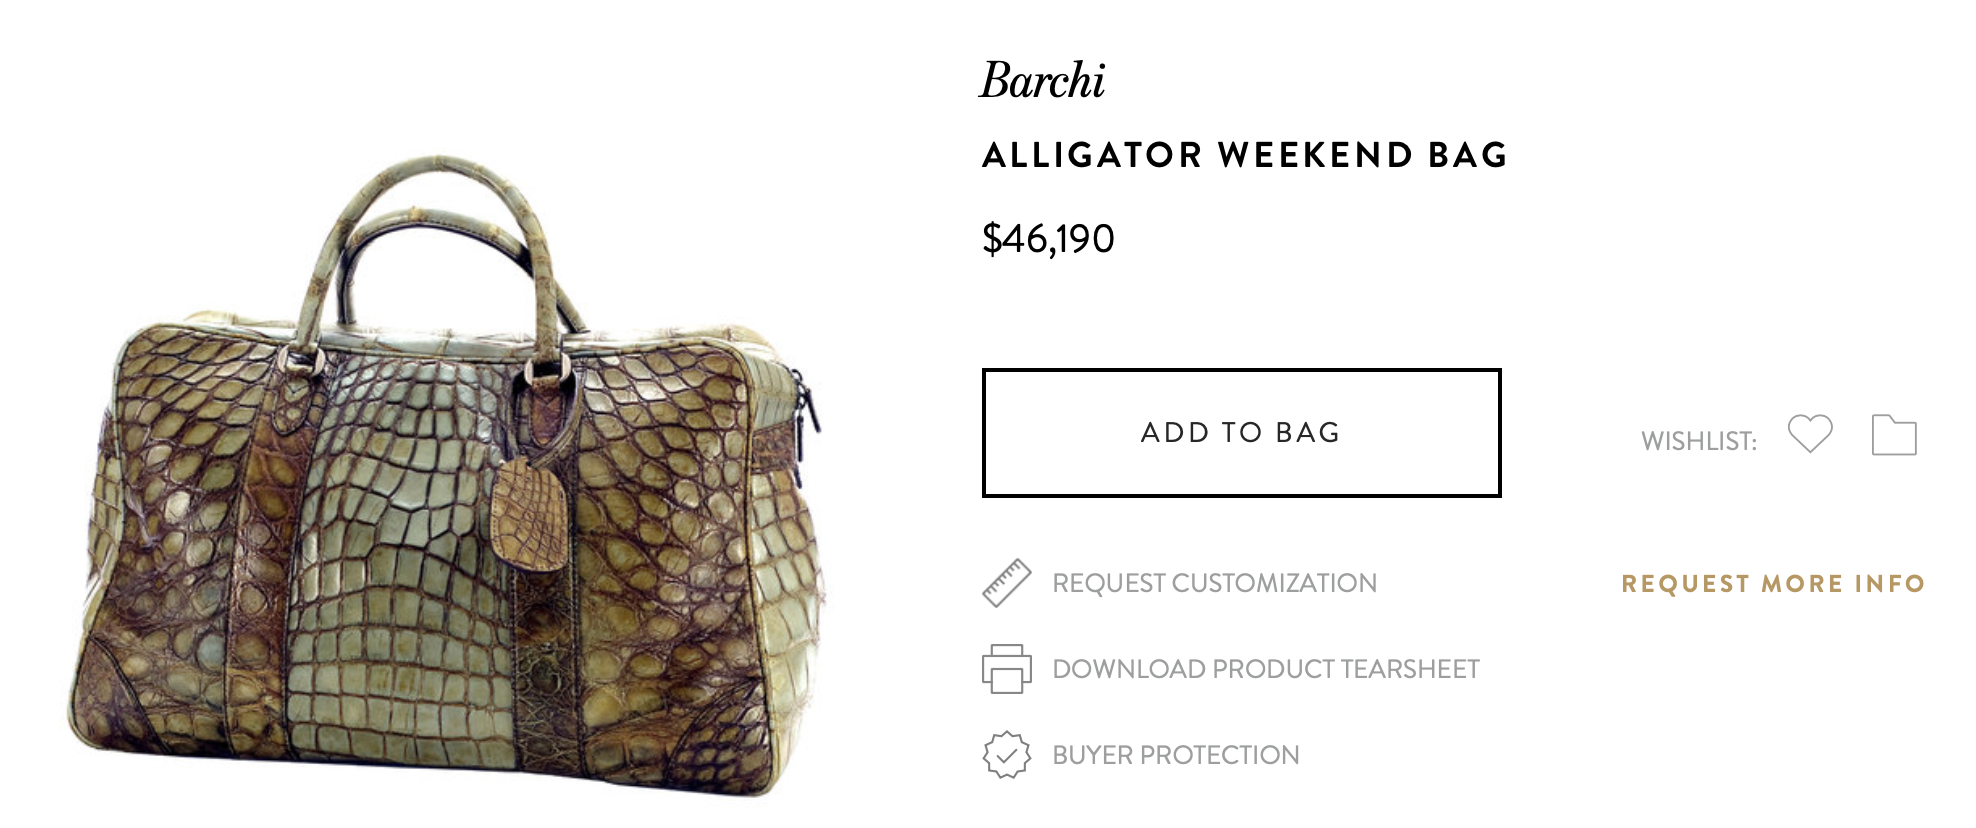
\includegraphics[width=0.8\textwidth]{figures/aBag.png}
		
	\end{center}
\end{frame}


%---------------------------------------%
% Case Study #3: Fashion                %
%---------------------------------------%
\begin{frame}[t]
\frametitle{Fashion: Reptile Skins}
\vspace{0.5cm}

	The use of wildlife for fashion has been controversial for a long time\\
	
	\vspace{0.4cm}
	
	Pressure from animal rights groups has reduced demand in some areas, but not others\\
	
	\vspace{0.25cm}
	
	\begin{center}
		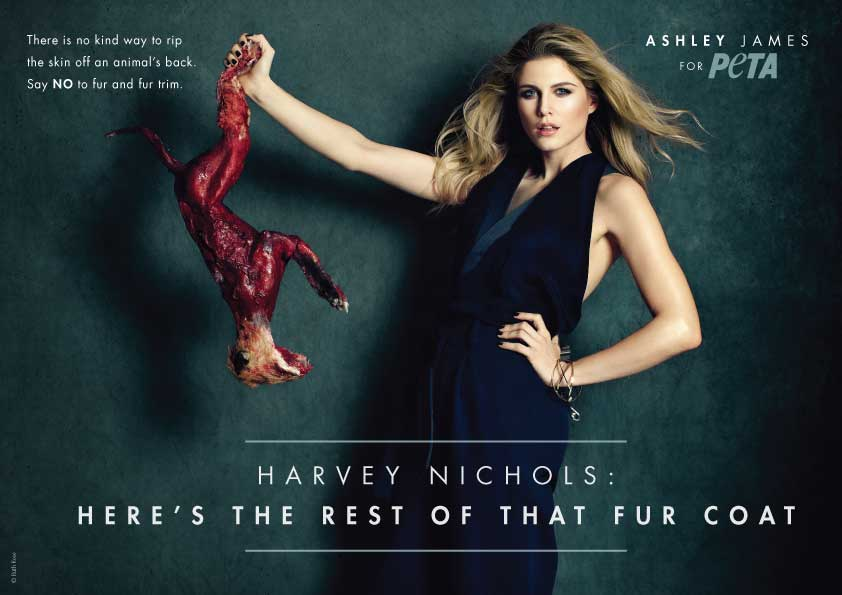
\includegraphics[width=0.6\textwidth]{figures/peta.jpg}
	\end{center}	
\end{frame}


%---------------------------------------%
% Case Study #3: Fashion                %
%---------------------------------------%
\begin{frame}[t]
\frametitle{Fashion: Reptile Skins}
\vspace{0.5cm}

	\begin{reference}{4mm}{92mm}
		\rule{1.5cm}{0.25pt}\\
		UNODC (2016) World Wildlife Crime Report: Trafficking in protected species.
	\end{reference}
	
	Despite these efforts, demand globally seems to be increasing
	
	\vspace{0.5cm}
	
	\begin{center}
		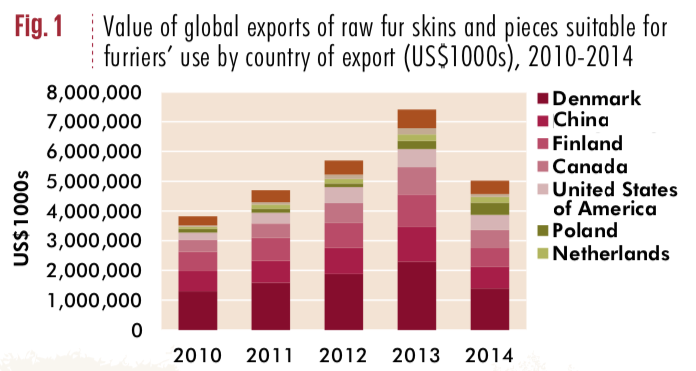
\includegraphics[width=0.8\textwidth]{figures/fashion_trends.png}
	\end{center}	
\end{frame}


%---------------------------------------%
% Case Study #3: Fashion                %
%---------------------------------------%
\begin{frame}[t]
\frametitle{Fashion: Reptile Skins}
\vspace{0.5cm}

	Fashion industry is very volatile\\
	\medskip
		\begin{itemize}
			\item What is in fashion now, may not be in the future\\
		\end{itemize}
	
	\vspace{0.4cm}
	
	Farming industry is very risky, and wild sources requires less investment\\
	\medskip
		\begin{itemize}
			\item Most sources are from the wild (mink is the main exception)
		\end{itemize}			
\end{frame}


%---------------------------------------%
% Case Study #3: Fashion                %
%---------------------------------------%
\begin{frame}[t]
\frametitle{Fashion: Reptile Skins}
\vspace{0.5cm}

	\begin{reference}{4mm}{92mm}
		\rule{1.5cm}{0.25pt}\\
		nsmink.ca\\
	\end{reference}

	Nova Scotia is a key mink farming area\\
	
	\vspace{0.5cm}
	
	\begin{center}
		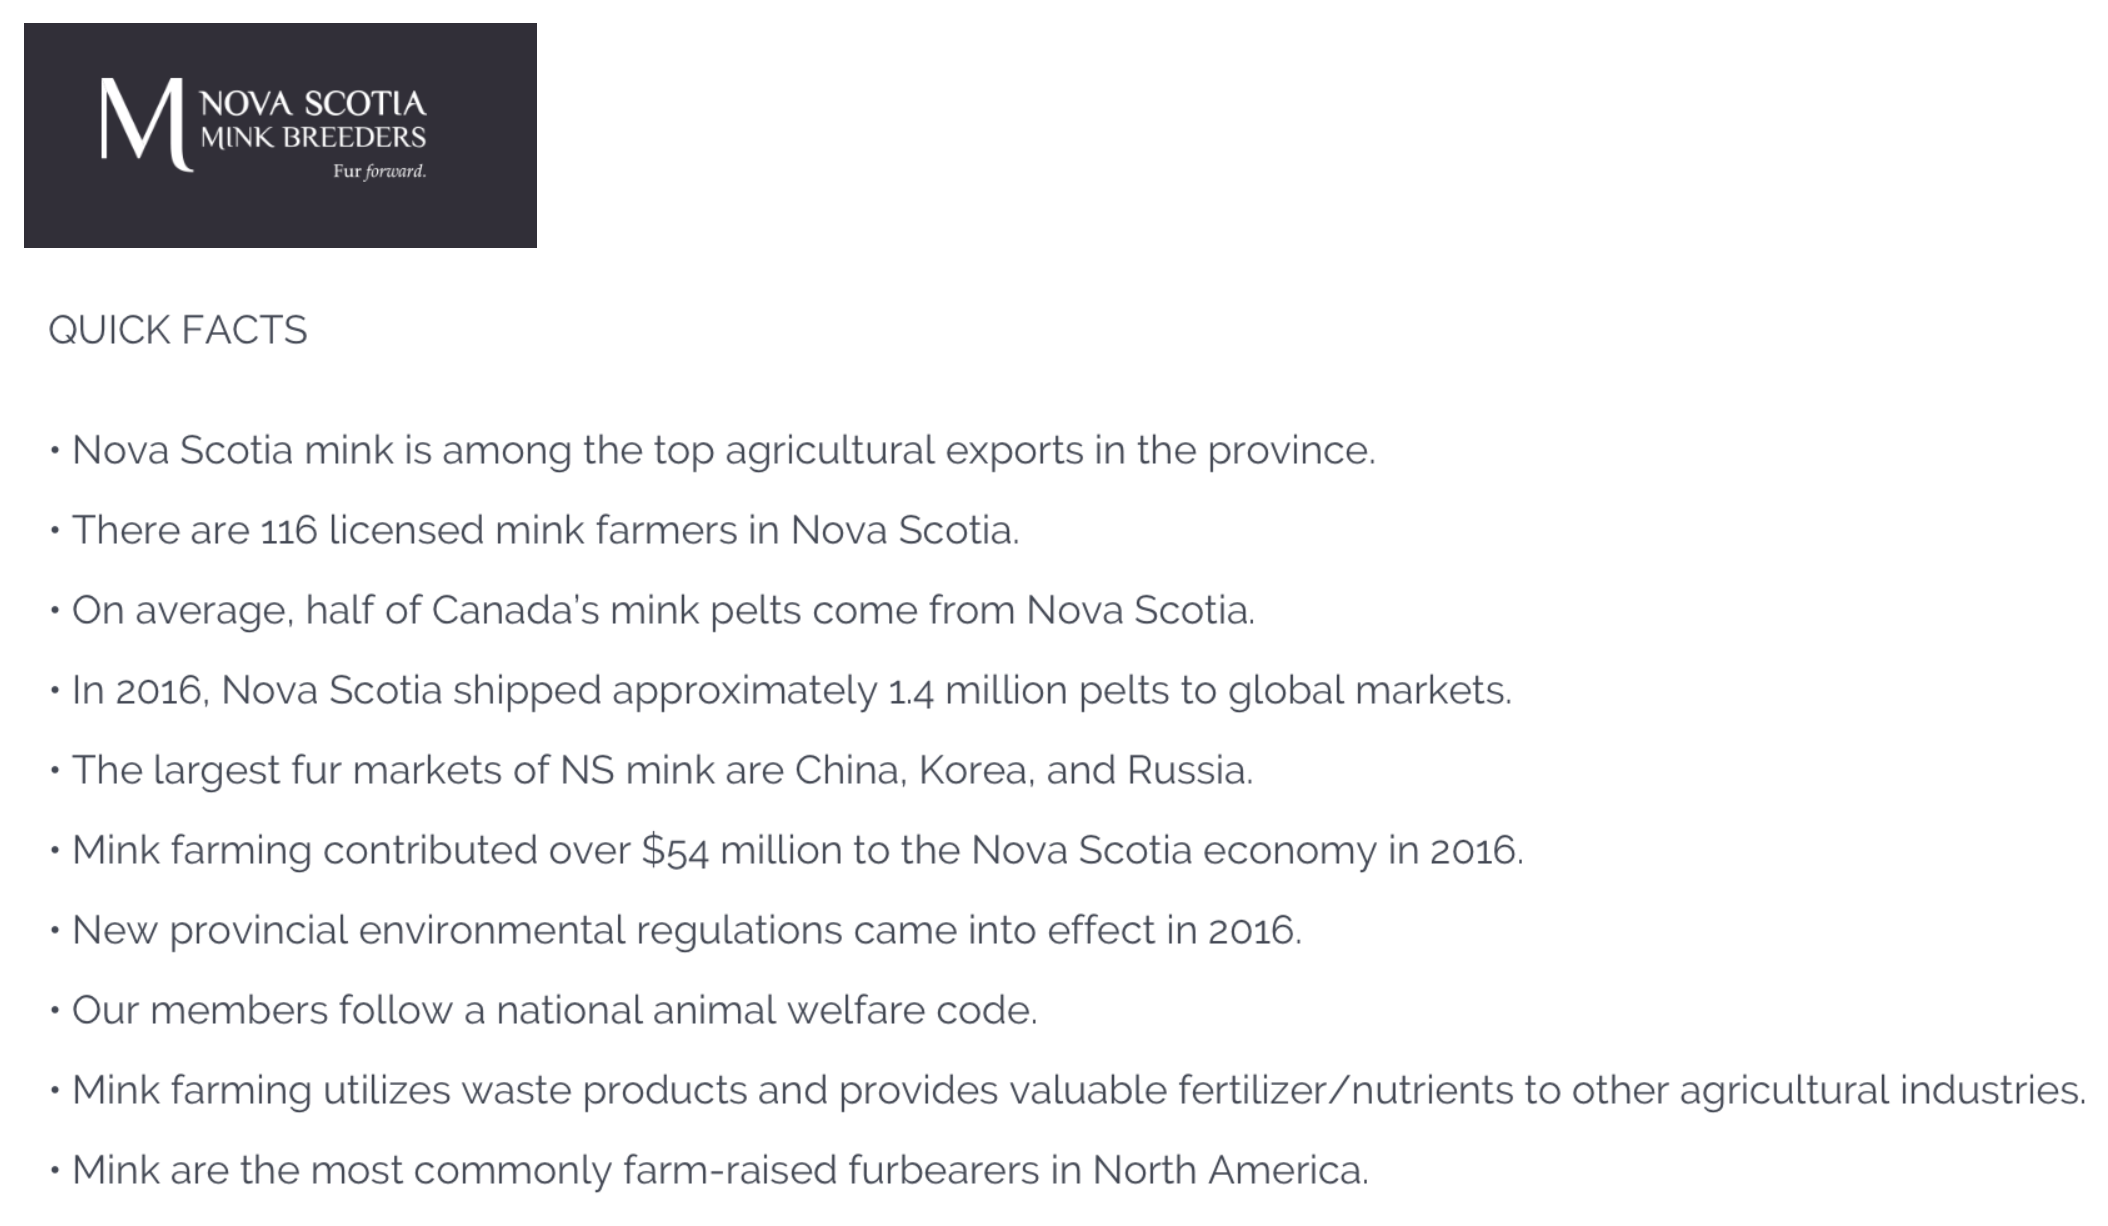
\includegraphics[width=0.9\textwidth]{figures/mink.png}
	\end{center}
\end{frame}


%---------------------------------------%
% Case Study #3: Fashion                %
%---------------------------------------%
\begin{frame}[t]
\frametitle{Fashion: Reptile Skins}
\vspace{0.5cm}

	\begin{reference}{4mm}{92mm}
		\rule{1.5cm}{0.25pt}\\
		1. UNODC (2016) World Wildlife Crime Report: Trafficking in protected species.
	\end{reference}
	
	The global market for reptile skin is immense\\
	\medskip
		\begin{itemize}
			\item In 2013, 3,500 metric tons, worth over \$650 million US, were imported globally$^{1}$
			\medskip
			\item Depending on species, represents 2--50 million animals
			\medskip
			\item One large python skin worth \$100 US$^{1}$
				\begin{itemize}
					\item Take $\sim$4 years to reach ``harvestable size'' - incentive to turn to the wild
				\end{itemize}
		\end{itemize}
\end{frame}


%---------------------------------------%
% Case Study #3: Fashion                %
%---------------------------------------%
\begin{frame}[t]
\frametitle{Fashion: Reptile Skins}
\vspace{0.5cm}

	\begin{reference}{4mm}{92mm}
		\rule{1.5cm}{0.25pt}\\
		1. UNODC (2016) World Wildlife Crime Report: Trafficking in protected species.
	\end{reference}
	
	Main reptiles traded for their skins:$^{1}$\\
	
	\begin{columns}[t]
		\begin{column}{0.6\textwidth}
			\begin{itemize}
			\item Crocodilians:
				\begin{itemize}
					\item Mississippi alligator
					\item Three species of caimans
					\item Four species of crocodiles
				\end{itemize}
			\medskip
			\item Snakes
				\begin{itemize}
					\item Three species of pythons
					\item The Indian rat snake
					\item The Javan spitting cobra
				\end{itemize}		
			\medskip
			\item Lizards
				\begin{itemize}
					\item Two species of monitors
					\item Two species of tegus
				\end{itemize}	
			\end{itemize}
		\end{column}
		
		\begin{column}{0.4\textwidth}
			\begin{center}
				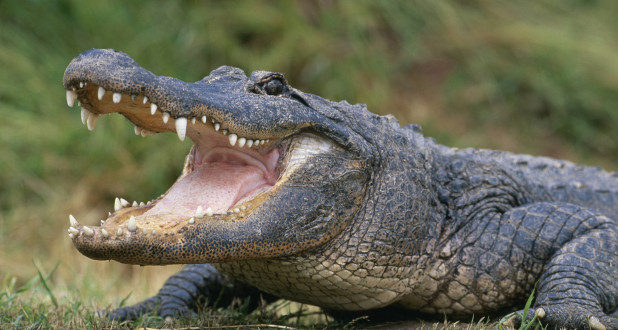
\includegraphics[width=0.7\textwidth]{figures/alligator.jpg}\\
				\vspace{0.25cm}
				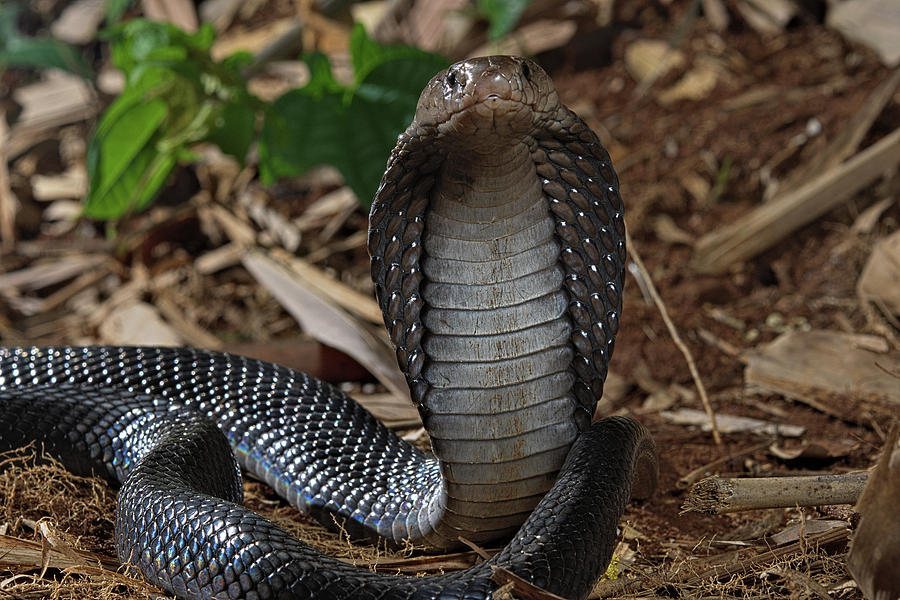
\includegraphics[width=0.7\textwidth]{figures/cobra.jpg}\\
				\vspace{0.25cm}
				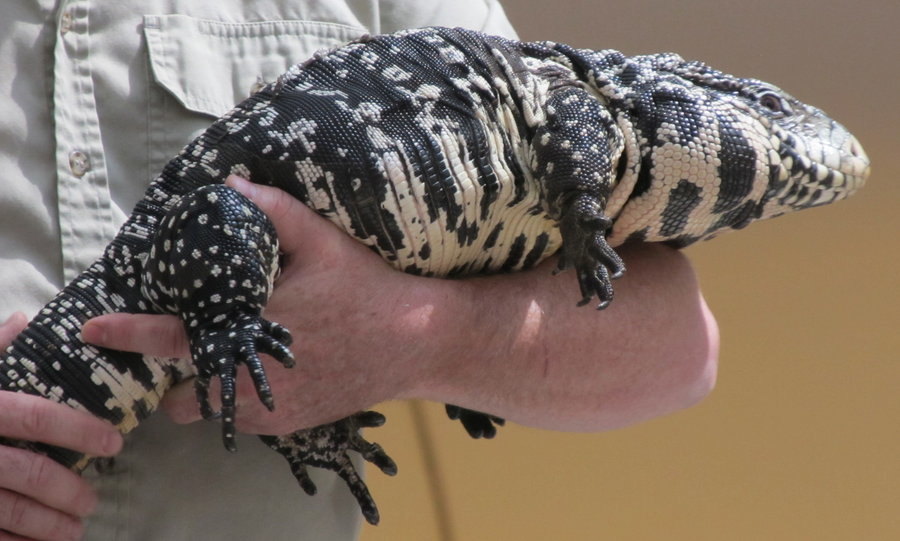
\includegraphics[width=0.7\textwidth]{figures/tegu.jpg}
			\end{center}
		\end{column}
	\end{columns}
		
\end{frame}


%---------------------------------------%
% Case Study #3: Fashion                %
%---------------------------------------%
\begin{frame}[t]
\frametitle{Fashion: Reptile Skins}
\vspace{0.25cm}

	\begin{reference}{4mm}{92mm}
		\rule{1.5cm}{0.25pt}\\
		UNODC (2016) World Wildlife Crime Report: Trafficking in protected species.
	\end{reference}
	

	\begin{center}
		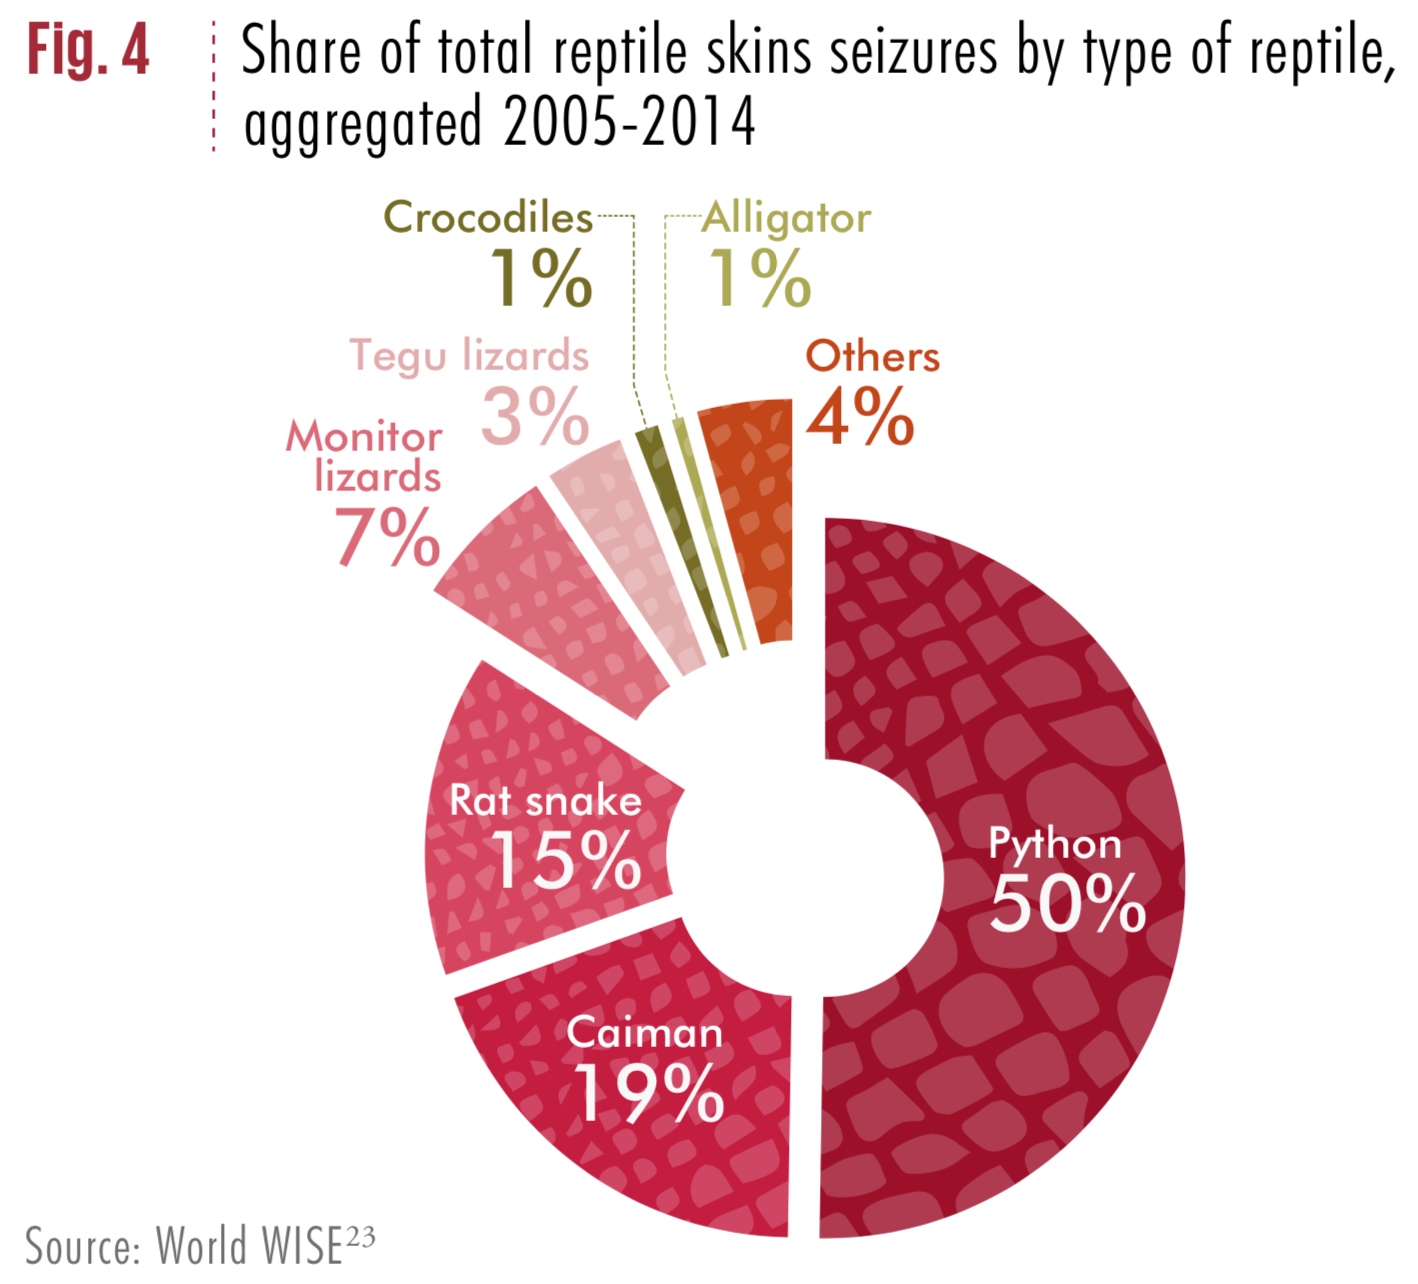
\includegraphics[width=0.7\textwidth]{figures/fashion_species.png}
	\end{center}
\end{frame}


%---------------------------------------%
% Case Study #3: Fashion                %
%---------------------------------------%
\begin{frame}[t]
\frametitle{Fashion: Reptile Skins}
\vspace{0.25cm}

	\begin{reference}{4mm}{92mm}
		\rule{1.5cm}{0.25pt}\\
		UNODC (2016) World Wildlife Crime Report: Trafficking in protected species.
	\end{reference}
	
	Many \textcolor{myblue}{source} countries involved, but Columbia and Indonesia represent 50\% of \emph{legal} trade. A bit different for the illegal trade\\
	
	\vspace{0.25cm} 

	\begin{columns}
		\begin{column}{0.5\textwidth}
			\begin{center}
				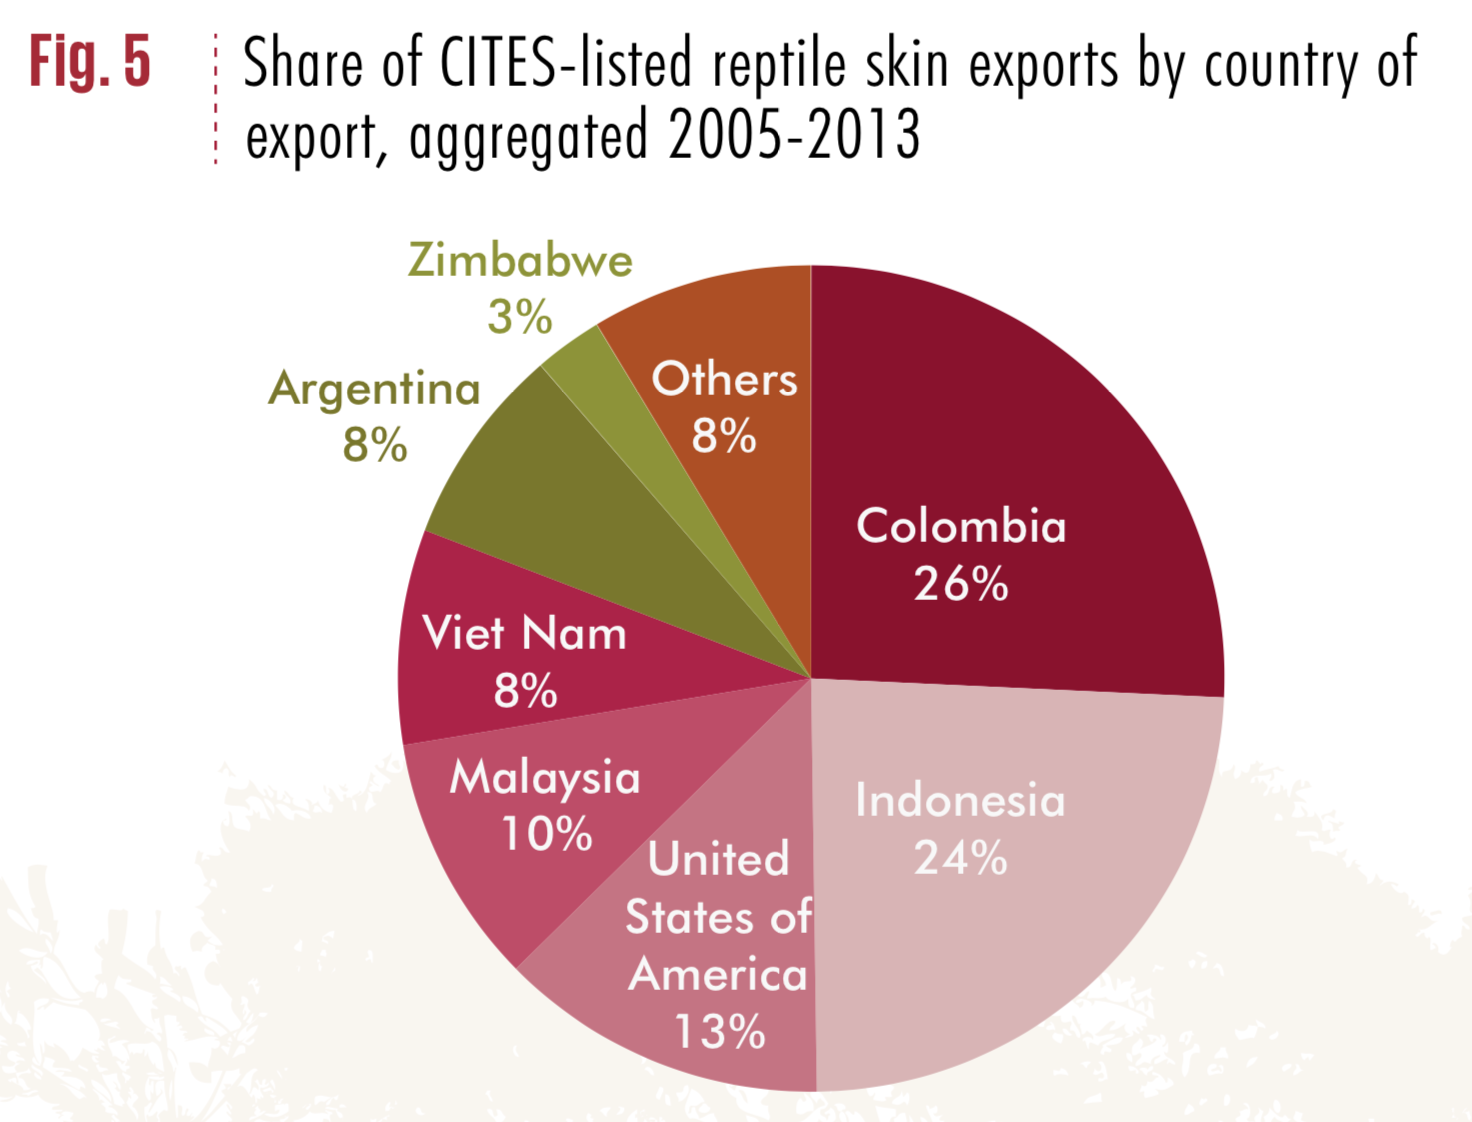
\includegraphics[width=1.0\textwidth]{figures/fashion_legal.png}
			\end{center}
		\end{column}
		
		\begin{column}{0.5\textwidth}
			\begin{center}
				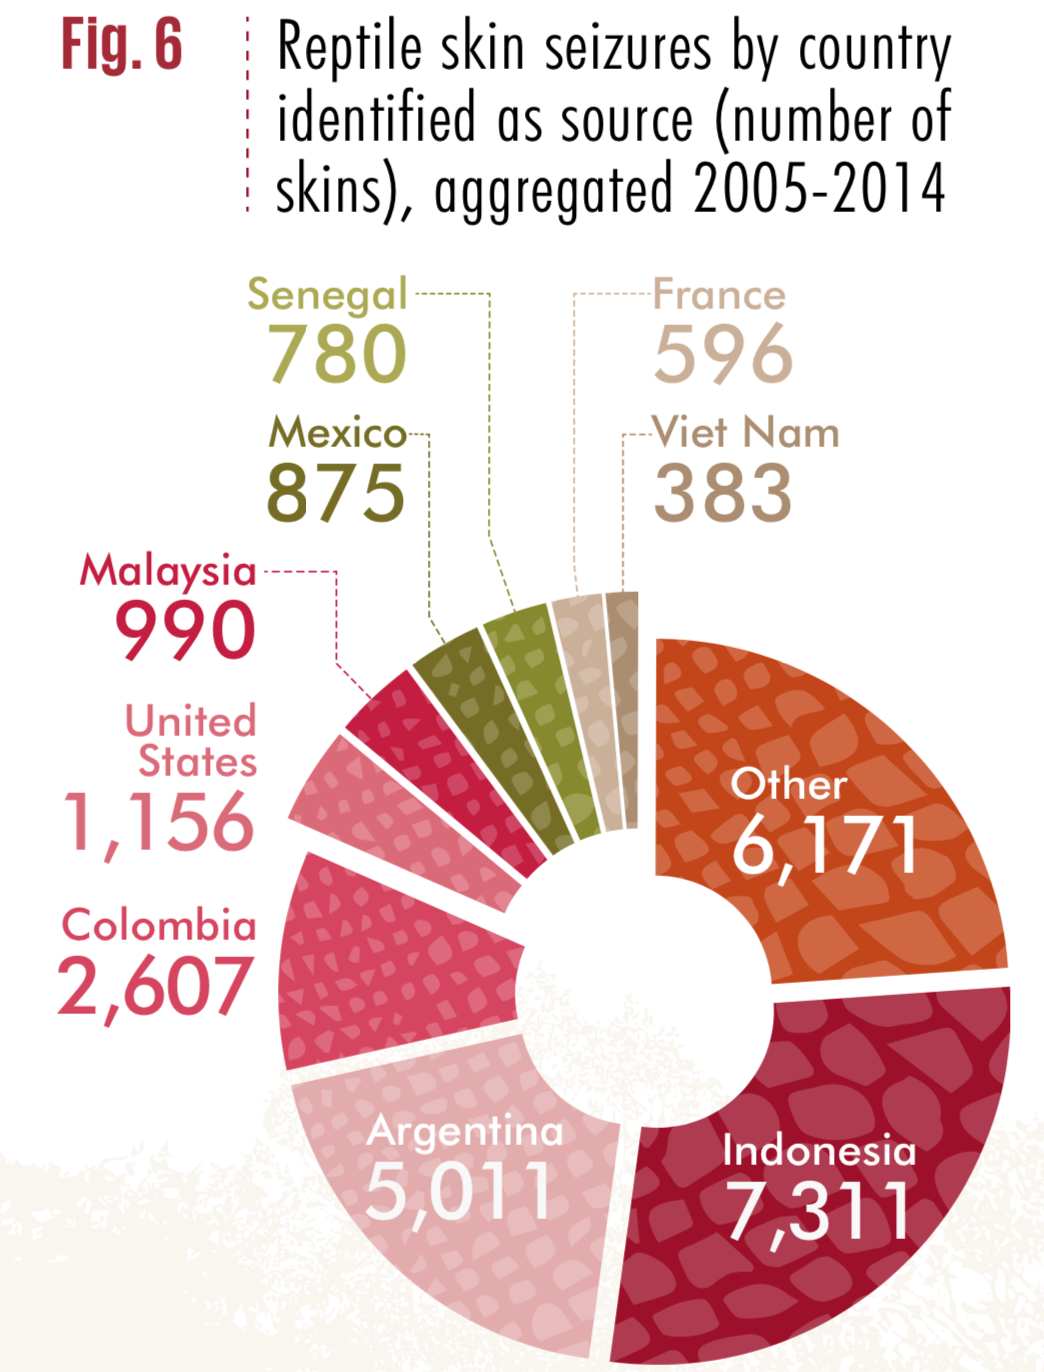
\includegraphics[width=0.7\textwidth]{figures/fashion_illegal.png}
			\end{center}
		\end{column}
	\end{columns}
\end{frame}


%---------------------------------------%
% Case Study #3: Fashion                %
%---------------------------------------%
\begin{frame}[t]
\frametitle{Fashion: Reptile Skins}
\vspace{0.25cm}

	\begin{reference}{4mm}{92mm}
		\rule{1.5cm}{0.25pt}\\
		UNODC (2016) World Wildlife Crime Report: Trafficking in protected species.
	\end{reference}
	
	Singapore the leading importer in the \emph{legal} trade, while Spain is the highest importer in the \emph{illegal} trade\\
	
	\vspace{0.25cm} 

	\begin{columns}
		\begin{column}{0.5\textwidth}
			\begin{center}
				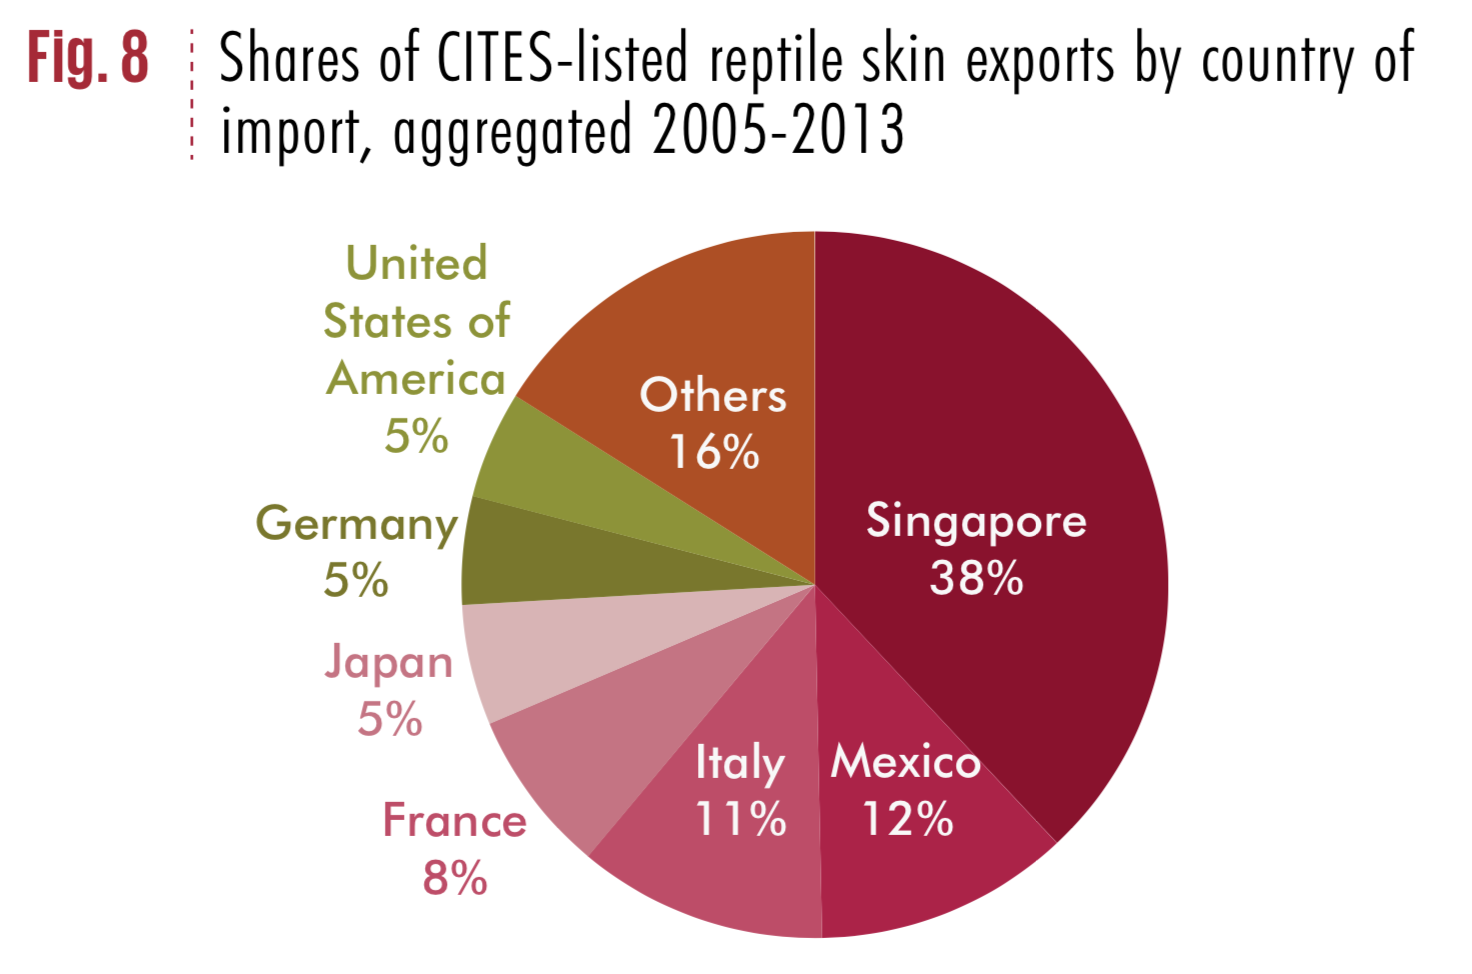
\includegraphics[width=1.0\textwidth]{figures/fashion_legal_import.png}
			\end{center}
		\end{column}
		
		\begin{column}{0.5\textwidth}
			\begin{center}
				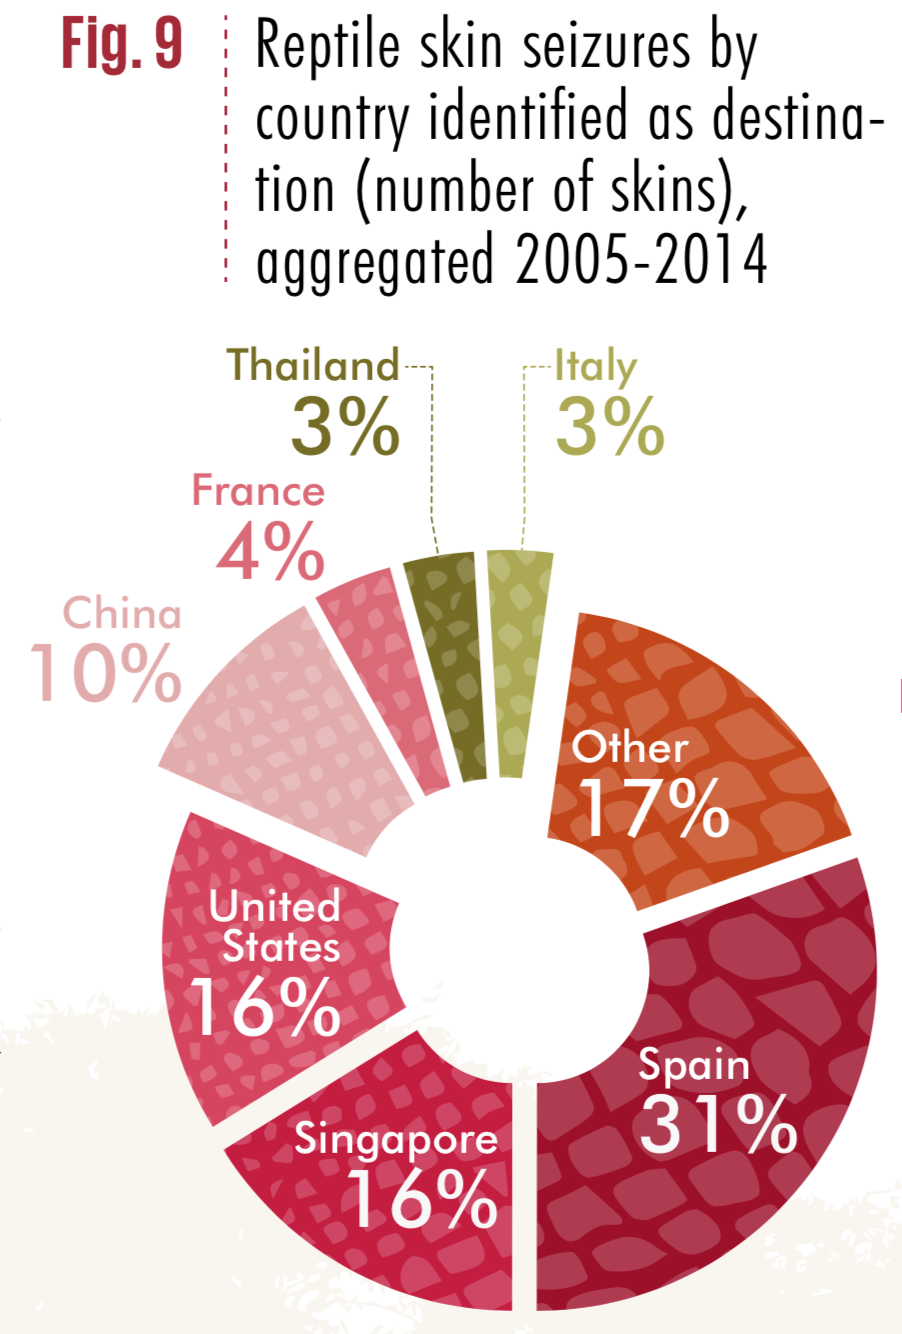
\includegraphics[width=0.7\textwidth]{figures/fashion_illegal_import.png}
			\end{center}
		\end{column}
	\end{columns}
\end{frame}


%---------------------------------------%
% Case Study #3: Fashion                %
%---------------------------------------%
\begin{frame}[t]
\frametitle{Fashion: Reptile Skins}
\vspace{0.25cm}

	\begin{reference}{4mm}{92mm}
		\rule{1.5cm}{0.25pt}\\
		UNODC (2016) World Wildlife Crime Report: Trafficking in protected species.
	\end{reference}
	
	\begin{center}
		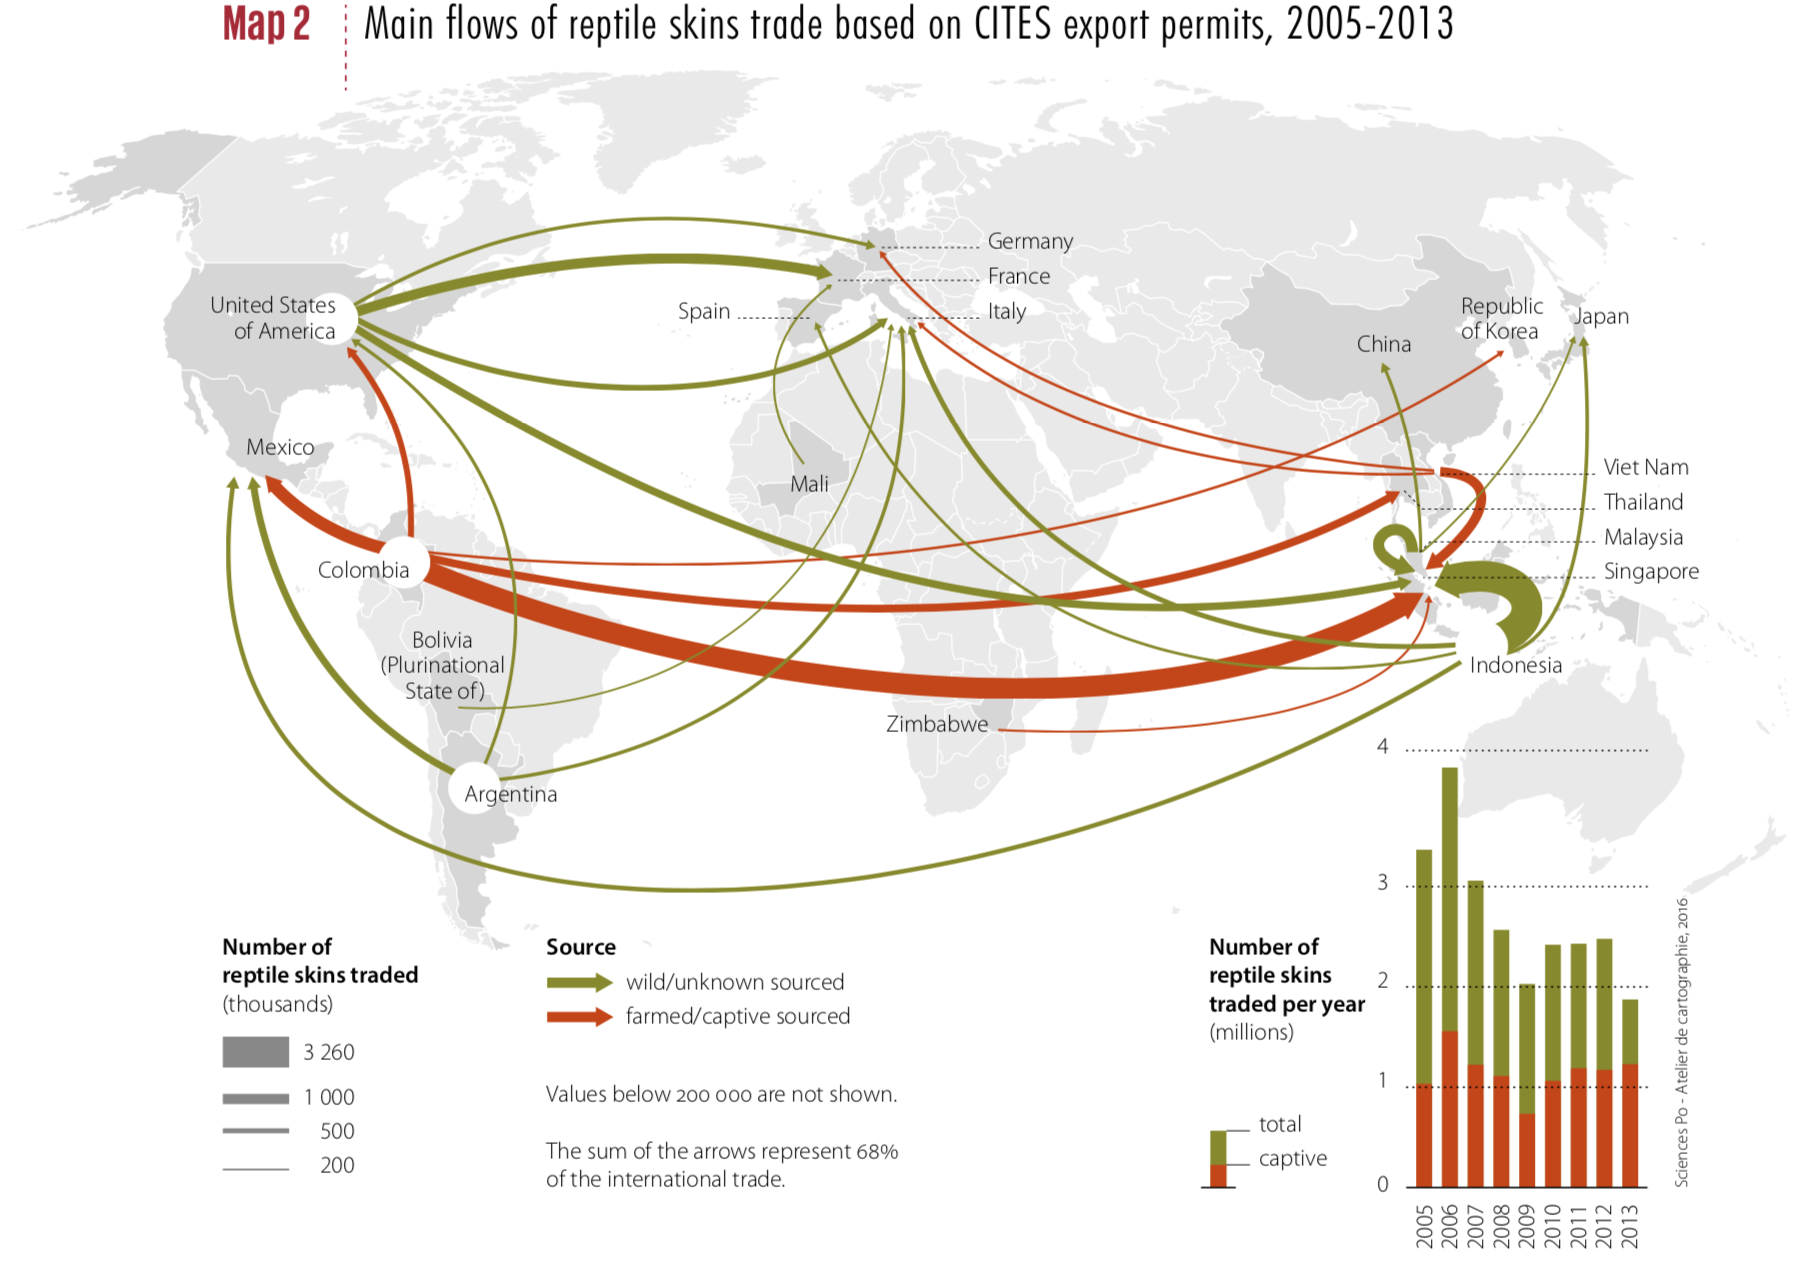
\includegraphics[width=1.0\textwidth]{figures/map3b.png}
	\end{center}
\end{frame}


%---------------------------------------%
% Case Study #3: Fashion                %
%---------------------------------------%
\begin{frame}[t]
\frametitle{Fashion: Reptile Skins}
\vspace{0.25cm}

	\begin{reference}{4mm}{92mm}
		\rule{1.5cm}{0.25pt}\\
		UNODC (2016) World Wildlife Crime Report: Trafficking in protected species.
	\end{reference}
	
	\begin{center}
		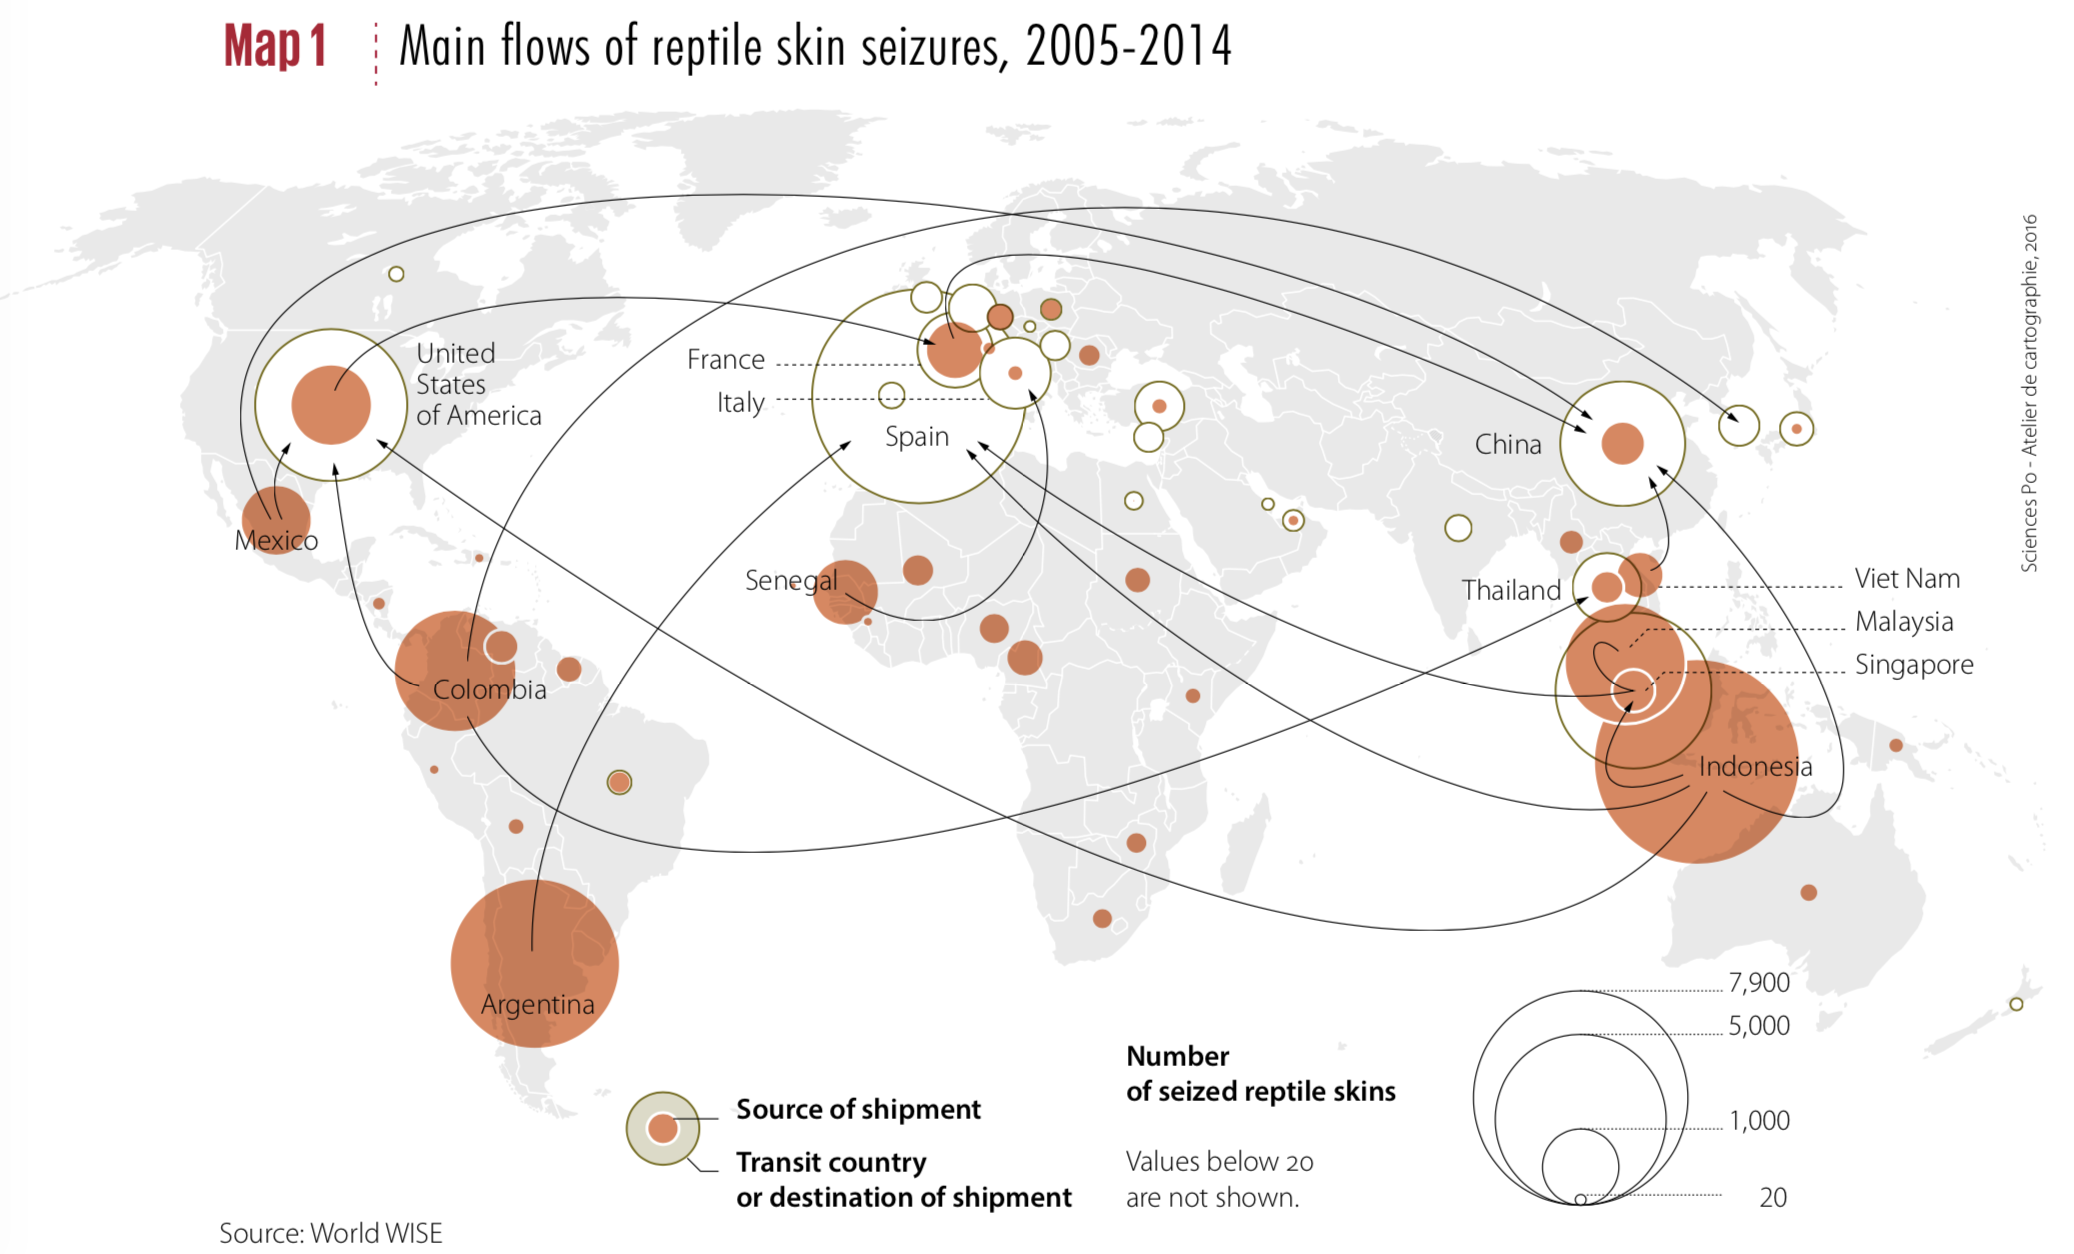
\includegraphics[width=1.0\textwidth]{figures/map3.png}
	\end{center}
\end{frame}


%---------------------------------------%
% Case Study #4: Cosmetics and Perfume  %
%---------------------------------------%
\begin{frame}
	\begin{center}
		\Large{\textbf{\textcolor{myblue}{Market \#4:\\ Cosmetics \& Perfume:}}}\normalsize{}\\ 
		
		\vspace{0.25cm}
		
		Agarwood Oud\\
		
		\vspace{0.5cm}
		
		\begin{columns}
			\begin{column}{0.5\textwidth}
				\begin{center}
					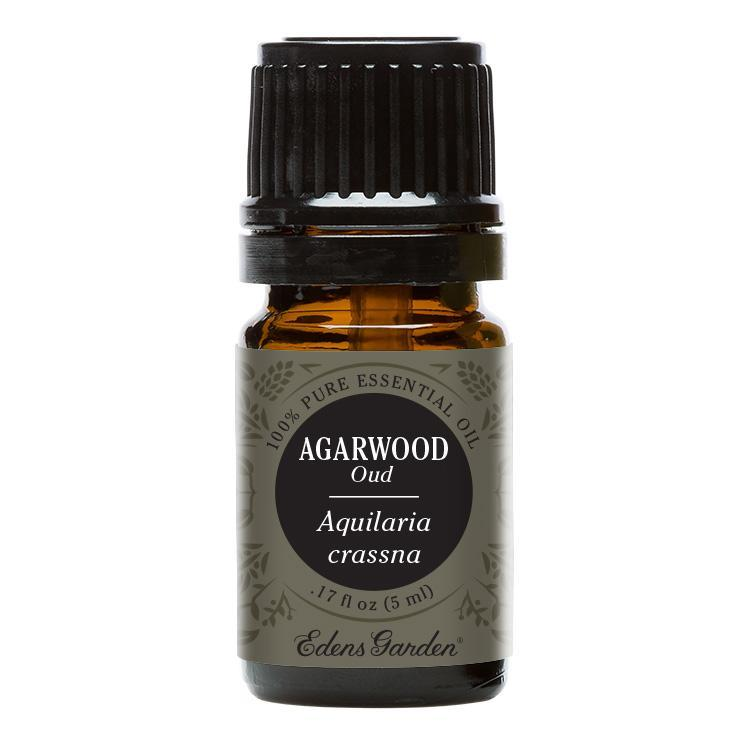
\includegraphics[width=0.8\textwidth]{figures/agarwood.jpg}
				\end{center}
			\end{column}	
			
			\begin{column}{0.5\textwidth}
				\begin{center}
					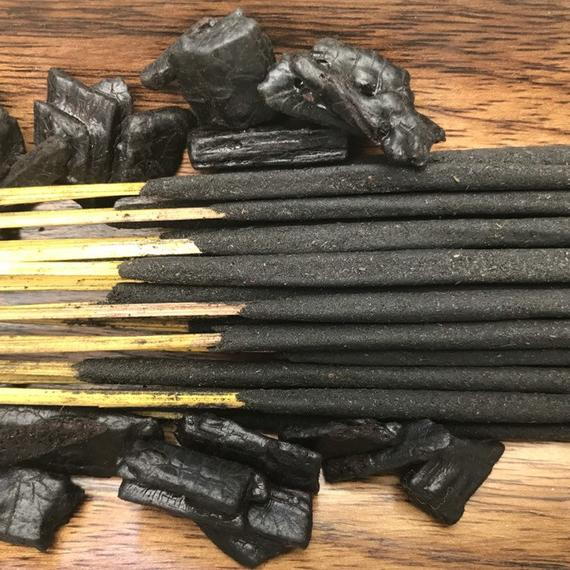
\includegraphics[width=0.8\textwidth]{figures/agarwood2.jpg}
				\end{center}
			\end{column}
		\end{columns}
	\end{center}
\end{frame}


%---------------------------------------%
% Case Study #4: Cosmetics and Perfume  %
%---------------------------------------%
\begin{frame}[t]
\frametitle{Agarwood oud}
\vspace{0.5cm}

	\begin{reference}{4mm}{92mm}
		\rule{1.5cm}{0.25pt}\\
		1. UNODC (2016) World Wildlife Crime Report: Trafficking in protected species.
	\end{reference}
	
	The global trade in essential oils, perfumes, cosmetics, and toiletries was worth $\sim$112 billion in 2014$^{1}$\\
	
	\vspace{0.5cm}
	
	It is estimated that $>$70\% of the European trade in medicinal and aromatic plants comes from the wild$^{1}$\\
	
	\vspace{0.5cm}
	
	Wild plant populations generally less well-documented than animal populations, making monitoring and tracking more difficult\\
	
	\vspace{0.5cm}
	
	Overharvesting tends to occur with species that are slow to recovery, as with many trees.
\end{frame}


%---------------------------------------%
% Case Study #4: Cosmetics and Perfume  %
%---------------------------------------%
\begin{frame}[t]
\frametitle{Agarwood oud}
\vspace{0.25cm}

	Agarwood, oud, jinkoh, and gaharu is not a particular type of tree, but rather a highly aromatic resin created by certain trees in response to infection by the mould (\emph{Phialophora parasitica})\\
	\smallskip
		\begin{itemize}
			\item Often trees of the genus \emph{Aquilaria}
		\end{itemize}
	
	\vspace{0.4cm}
	
	The resin-embedded wood is valued for its fragrance, and is used in incense and perfumes\\
	\smallskip
		\begin{itemize}
			\item Has become important in many ``eastern'' religious customs, especially in Muslim, Hindu, and Buddhist traditions
		\end{itemize}
	
	\begin{columns}
		\begin{column}{0.5\textwidth}
			\begin{center}
				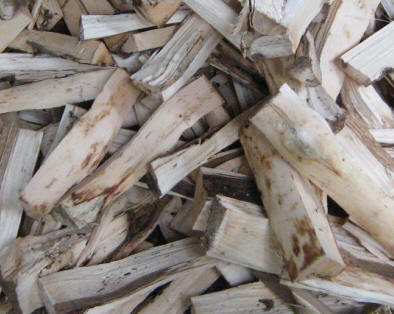
\includegraphics[width=0.5\textwidth]{figures/agarwood1.jpg}\\
				\emph{Uninfected agarwood}
			\end{center}
		\end{column}
		
		\begin{column}{0.5\textwidth}
			\begin{center}
				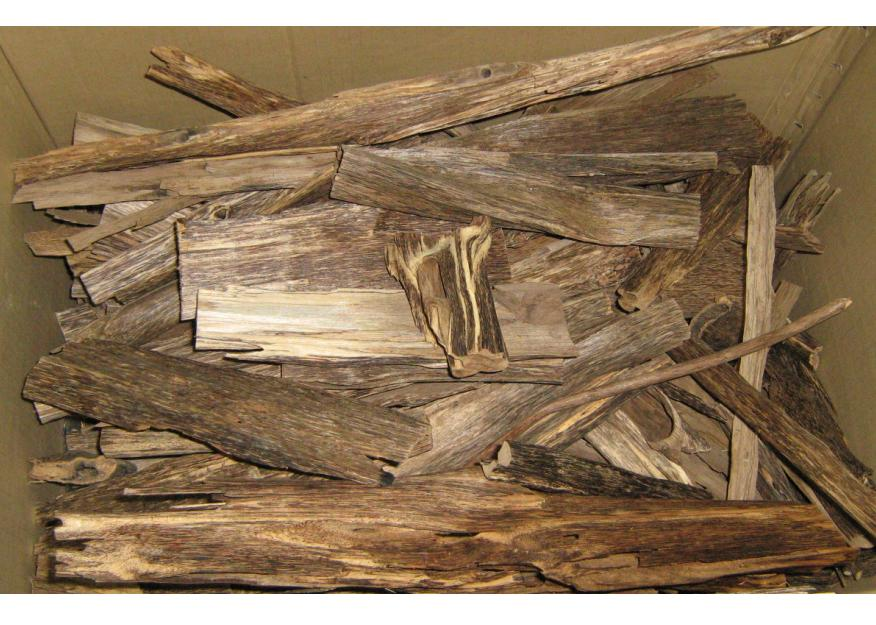
\includegraphics[width=0.6\textwidth]{figures/agarwood3.jpg}\\
				\emph{Infected agarwood}
			\end{center}
		\end{column}
	\end{columns}
\end{frame}


%---------------------------------------%
% Case Study #4: Cosmetics and Perfume  %
%---------------------------------------%
\begin{frame}[t]
\frametitle{Agarwood oud}
\vspace{0.5cm}

	\begin{reference}{4mm}{92mm}
		\rule{1.5cm}{0.25pt}\\
		1. UNODC (2016) World Wildlife Crime Report: Trafficking in protected species.
	\end{reference}

	Primary threat to these species is illegal harvesting for this trade\\
	
	\vspace{0.5cm}
	
	1 kg of high-quality oud chips worth hundreds of thousands of dollars$^{1}$\\
	
	\vspace{0.5cm}

	Only a small fraction of trees are infected
	\smallskip
		\begin{itemize}
			\item Difficult to tell before harvesing
			\smallskip
			\item Many trees killed without being used
		\end{itemize}
\end{frame}


%---------------------------------------%
% Case Study #4: Cosmetics and Perfume  %
%---------------------------------------%
\begin{frame}[t]
\frametitle{Agarwood oud}
\vspace{0.5cm}

	\begin{reference}{4mm}{92mm}
		\rule{1.5cm}{0.25pt}\\
		UNODC (2016) World Wildlife Crime Report: Trafficking in protected species.
	\end{reference}

	Demand is increasing rapidly
		\smallskip
		\begin{itemize}
			\item Increased pressure on wild populations
			\smallskip
			\item Development of cultivated sources
		\end{itemize}
	
	\vspace{0.25cm}
	
	\begin{center}
		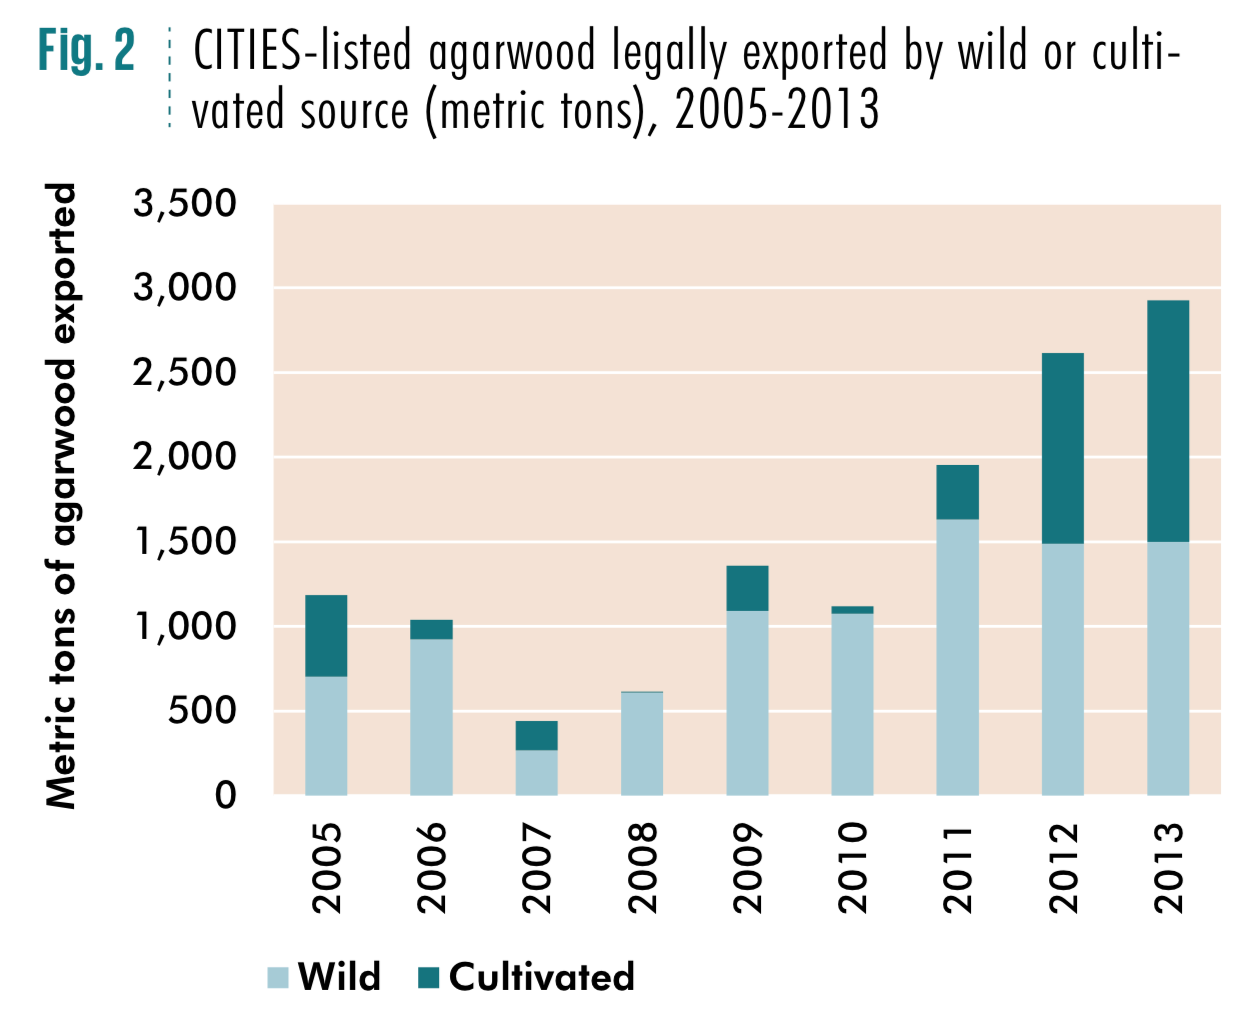
\includegraphics[width=0.6\textwidth]{figures/agarwood_trends.png}
	\end{center}	
\end{frame}


%---------------------------------------%
% Case Study #4: Cosmetics and Perfume  %
%---------------------------------------%
\begin{frame}[t]
\frametitle{Agarwood oud}
\framesubtitle{Legal trade}
\vspace{0.5cm}

	\begin{reference}{4mm}{92mm}
		\rule{1.5cm}{0.25pt}\\
		UNODC (2016) World Wildlife Crime Report: Trafficking in protected species.
	\end{reference}

	Most agarwood comes from countries in southeast Asia\\
	
	\vspace{0.25cm}
	
	\begin{center}
		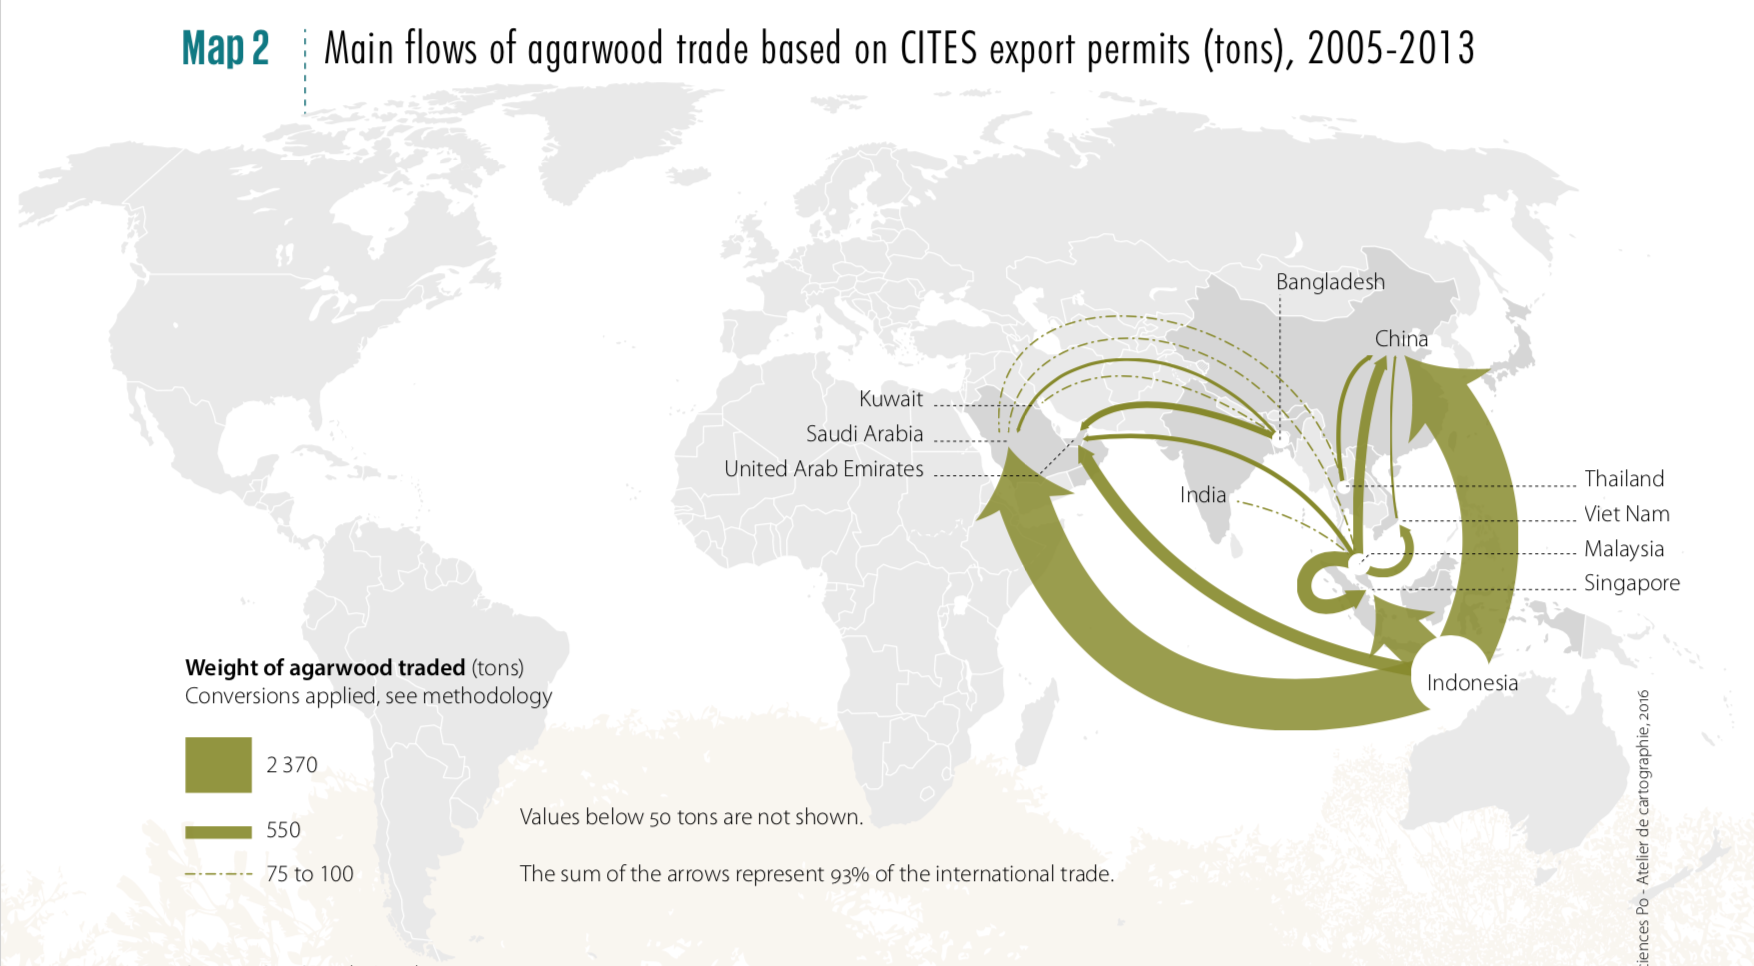
\includegraphics[width=0.9\textwidth]{figures/map4a.png}
	\end{center}	
\end{frame}


%---------------------------------------%
% Case Study #4: Cosmetics and Perfume  %
%---------------------------------------%
\begin{frame}[t]
\frametitle{Agarwood oud}
\framesubtitle{Legal trade}
\vspace{0.5cm}

	\begin{reference}{4mm}{92mm}
		\rule{1.5cm}{0.25pt}\\
		UNODC (2016) World Wildlife Crime Report: Trafficking in protected species.
	\end{reference}

	\begin{columns}
		\begin{column}{0.5\textwidth}
			\begin{center}
				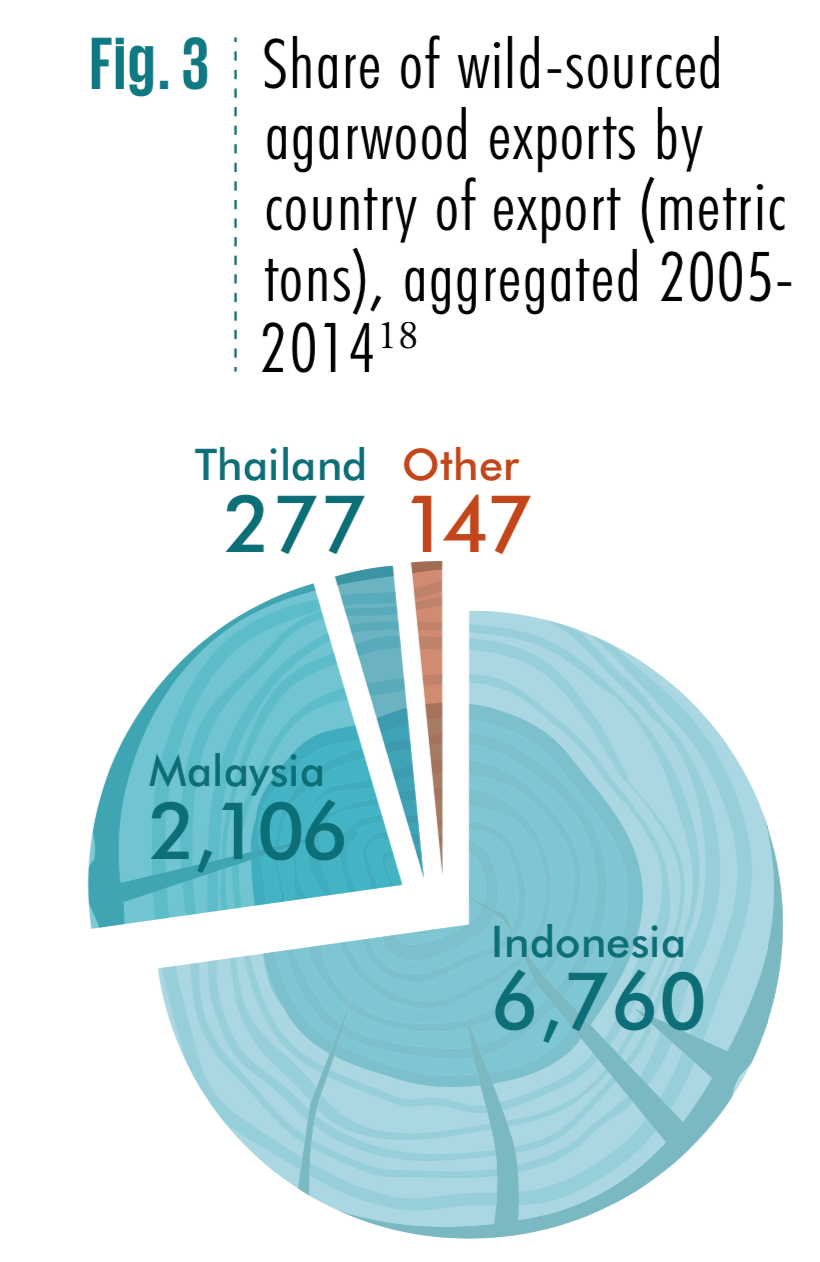
\includegraphics[width=0.6\textwidth]{figures/agarwood_legal_export.png}
			\end{center}
		\end{column}
		
		\begin{column}{0.5\textwidth}
			\begin{center}
				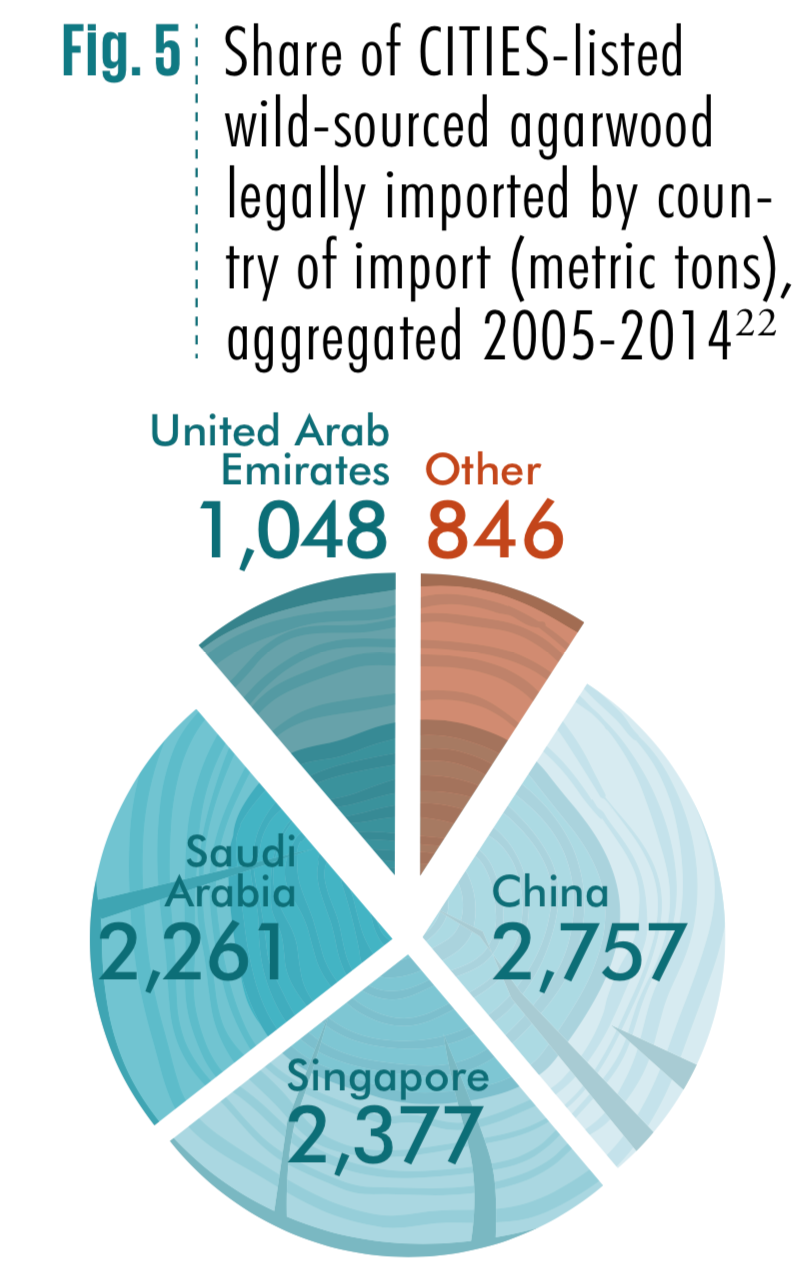
\includegraphics[width=0.6\textwidth]{figures/agarwood_legal_import.png}
			\end{center}
		\end{column}
	\end{columns}
\end{frame}


%---------------------------------------%
% Case Study #4: Cosmetics and Perfume  %
%---------------------------------------%
\begin{frame}[t]
\frametitle{Agarwood oud}
\framesubtitle{Illegal trade}
\vspace{0.5cm}

	\begin{reference}{4mm}{92mm}
		\rule{1.5cm}{0.25pt}\\
		UNODC (2016) World Wildlife Crime Report: Trafficking in protected species.
	\end{reference}
	
	\vspace{0.25cm}
	
	\begin{center}
		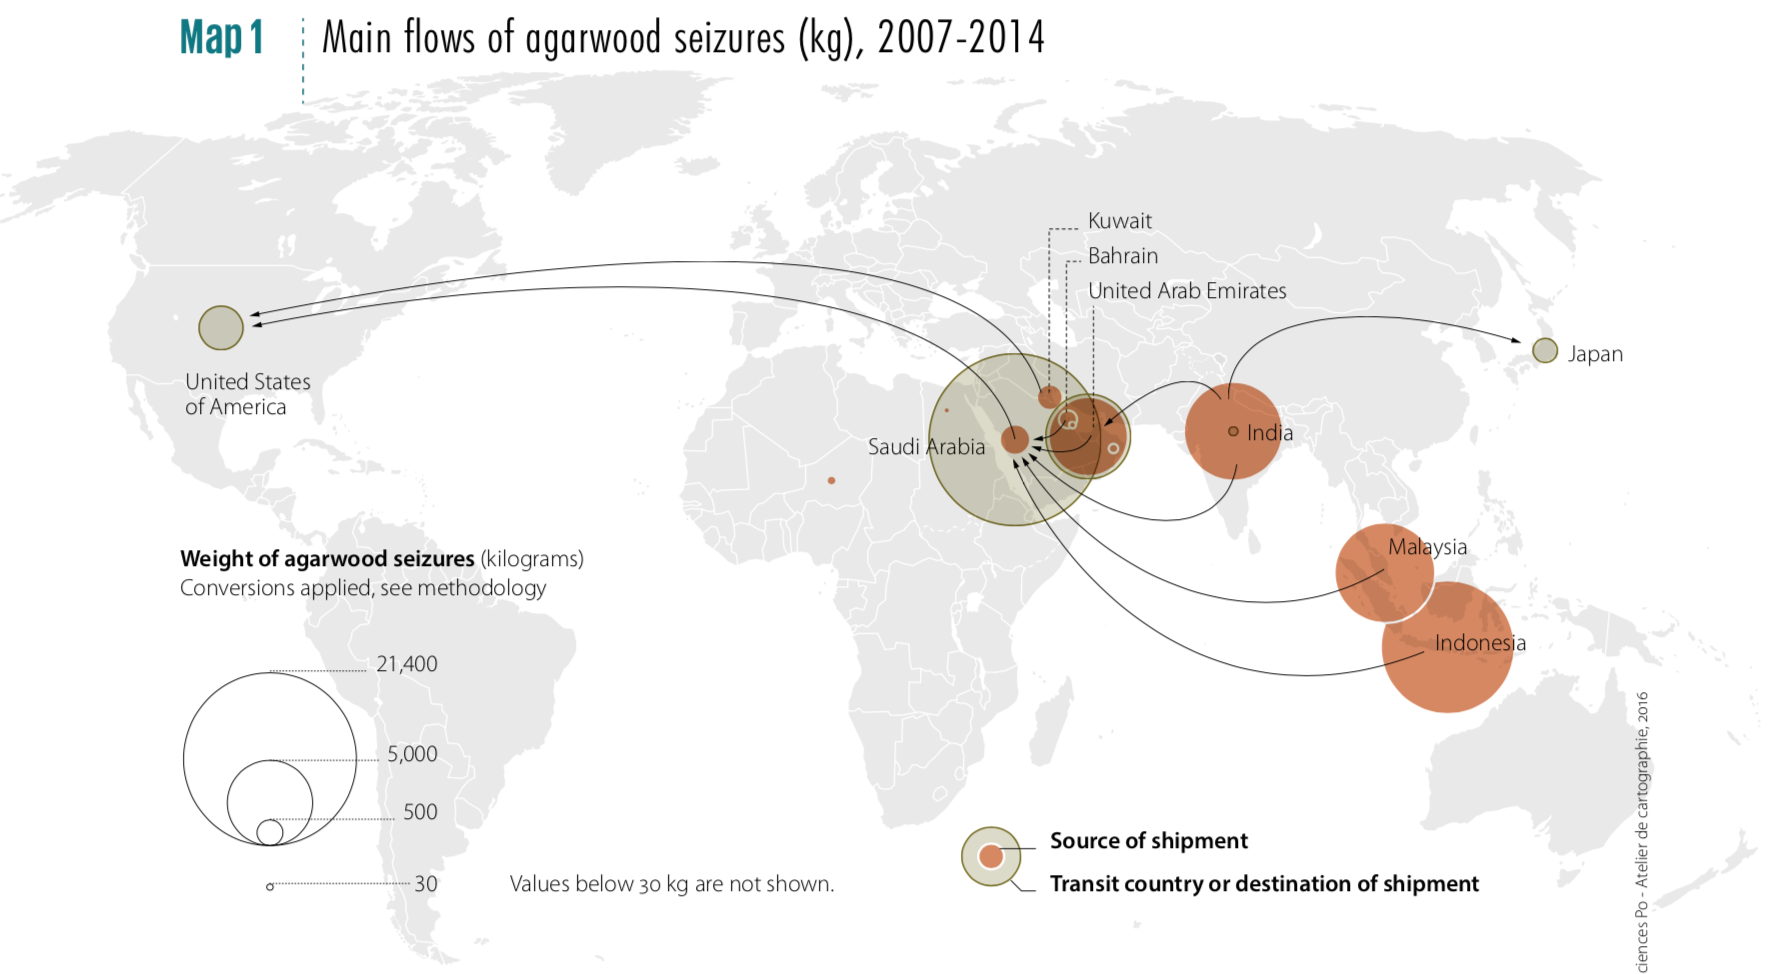
\includegraphics[width=1.0\textwidth]{figures/map4b.png}
	\end{center}	
\end{frame}


%---------------------------------------%
% Case Study #4: Cosmetics and Perfume  %
%---------------------------------------%
\begin{frame}[t]
\frametitle{Agarwood oud}
\framesubtitle{Illegal trade}
\vspace{0.5cm}

	\begin{reference}{4mm}{92mm}
		\rule{1.5cm}{0.25pt}\\
		UNODC (2016) World Wildlife Crime Report: Trafficking in protected species.
	\end{reference}

	\begin{columns}
		\begin{column}{0.5\textwidth}
			\begin{center}
				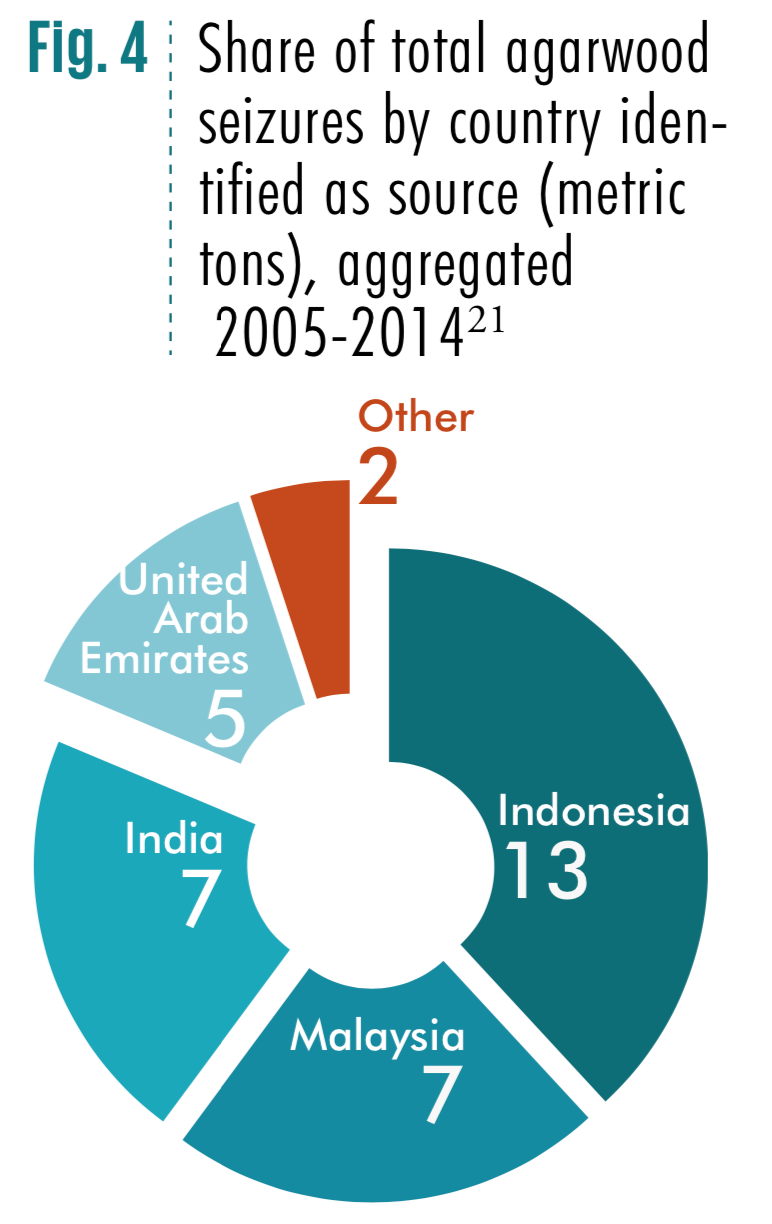
\includegraphics[width=0.6\textwidth]{figures/agarwood_illegal_export.png}
			\end{center}
		\end{column}
		
		\begin{column}{0.5\textwidth}
			\begin{center}
				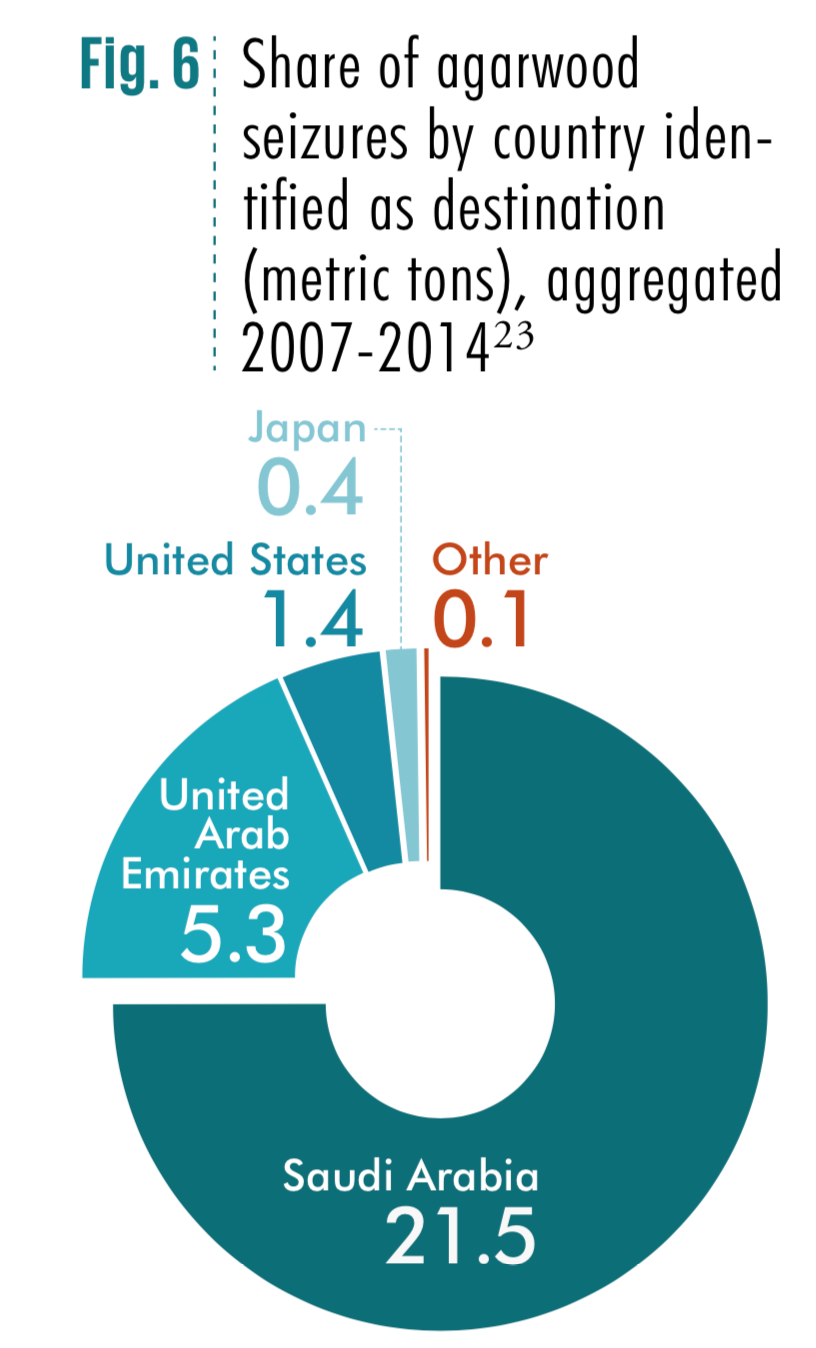
\includegraphics[width=0.6\textwidth]{figures/agarwood_illegal_import.png}
			\end{center}
		\end{column}
	\end{columns}
\end{frame}


%--------------------------------------------%
% Case Study #5: Food, Tonics, & Medicines   %
%--------------------------------------------%
\begin{frame}
	\begin{center}
		\Large{\textbf{\textcolor{myblue}{Market \#5:\\ Food, Tonics, \& Medicines:}}}\normalsize{}\\ 
		
		\vspace{0.25cm}
		
		Pangolin scales\\
		
		\vspace{0.5cm}
		
		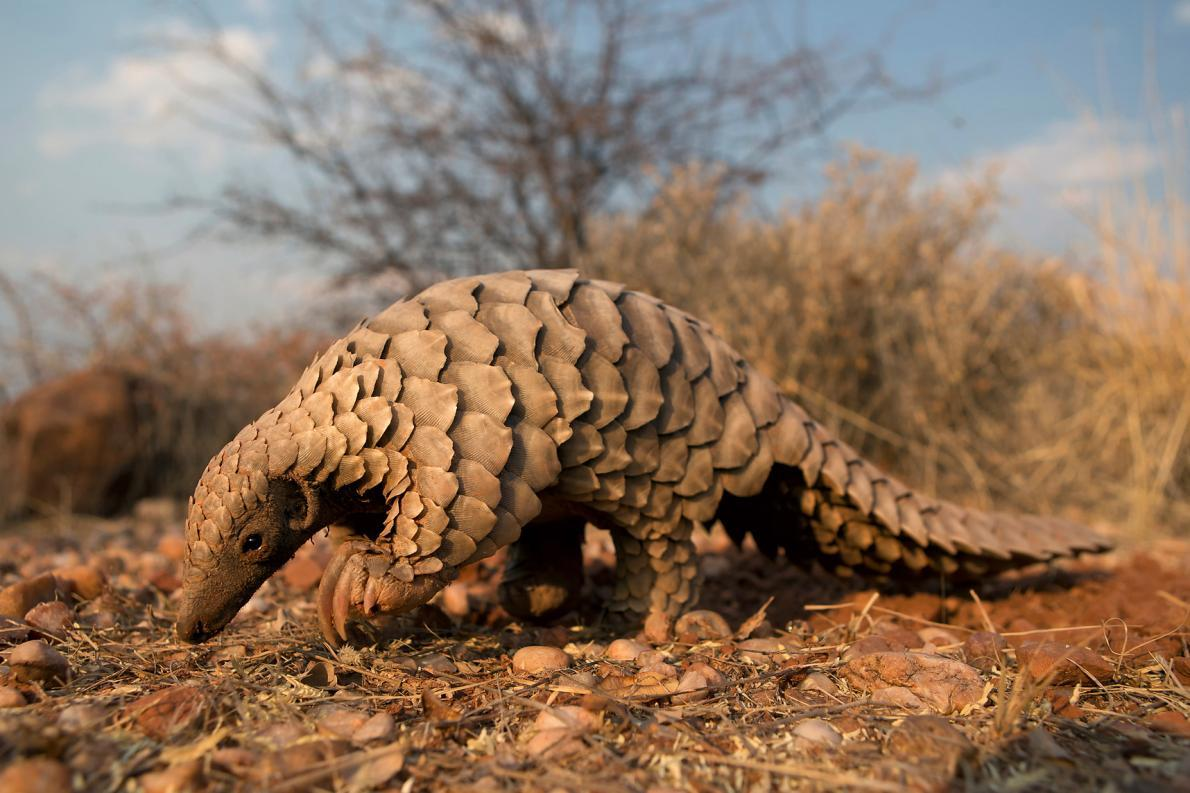
\includegraphics[width=0.7\textwidth]{figures/pangolin.jpg}
	\end{center}
\end{frame}


%--------------------------------------------%
% Case Study #5: Food, Tonics, & Medicines   %
%--------------------------------------------%
\begin{frame}[t]
\frametitle{Food, Tonics, \& Medicines}
\vspace{0.5cm}
	
	\begin{reference}{4mm}{92mm}
		\rule{1.5cm}{0.25pt}\\
		Graham-Rowe (2012) \emph{Nature} \textbf{480}: S101--S103
	\end{reference}
	
	Arguably the largest market/risk for \textcolor{myblue}{animals} involved in wildlife trade\\
	
	\vspace{0.25cm}
	
	\begin{center}
		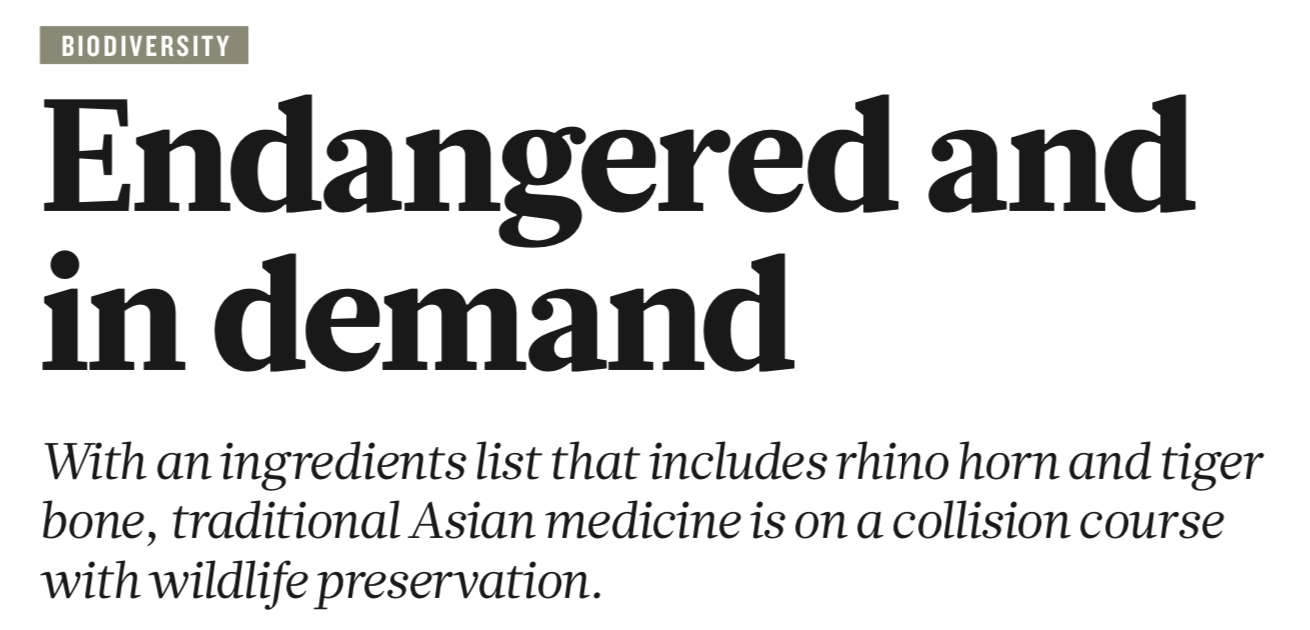
\includegraphics[width=0.7\textwidth]{figures/asian_medicine.png}
	\end{center}
\end{frame}


%--------------------------------------------%
% Case Study #5: Food, Tonics, & Medicines   %
%--------------------------------------------%
\begin{frame}[t]
\frametitle{Food, Tonics, \& Medicines}
\vspace{0.5cm}
	
	Are a great example of convergent evolution\\
	
	\vspace{0.5cm}
	
	\begin{columns}
		\begin{column}{0.5\textwidth}
			\begin{center}
				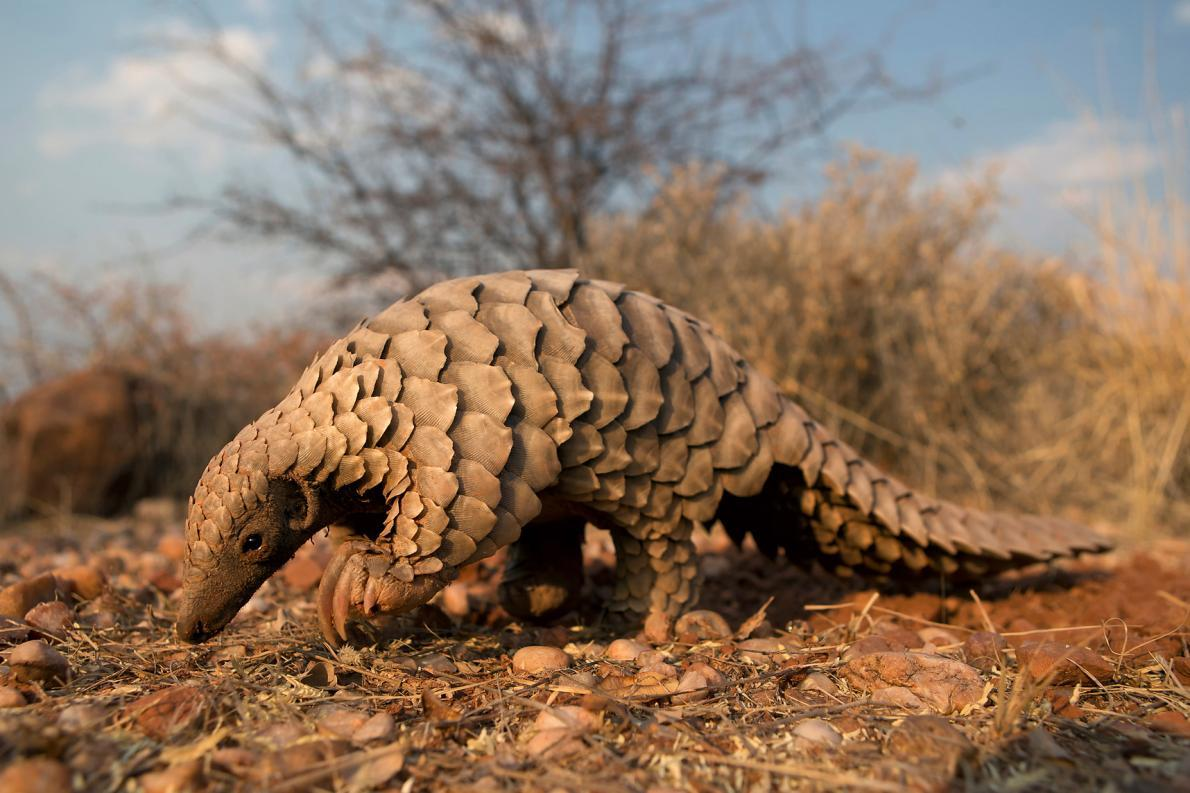
\includegraphics[width=0.9\textwidth]{figures/pangolin.jpg}
			\end{center}
		\end{column}
		
		\begin{column}{0.5\textwidth}
			\begin{center}
				\includegraphics[width=0.9\textwidth]{figures/armadillo.jpg}
			\end{center}
		\end{column}		
	\end{columns}
\end{frame}


%--------------------------------------------%
% Case Study #5: Food, Tonics, & Medicines   %
%--------------------------------------------%
\begin{frame}[t]
\frametitle{Food, Tonics, \& Medicines}
\vspace{0.25cm}
	
	Are 8 species:
		\smallskip
		\begin{itemize}
			\item 4 in Africa
			\smallskip
			\item 4 in Asia
		\end{itemize}
	
	\vspace{0.25cm}
	
	\begin{center}
		\includegraphics[width=0.65\textwidth]{figures/pangolin_species.png}
	\end{center}
\end{frame}


%--------------------------------------------%
% Case Study #5: Food, Tonics, & Medicines   %
%--------------------------------------------%
\begin{frame}[t]
\frametitle{Food, Tonics, \& Medicines}
\vspace{0.5cm}
	
	Scales are used in traditional medicine (primarily China \& Vietnam)\\
	
	\vspace{0.5cm}
	
	Demand for scales, and large numbers killed, have raised international concern
\end{frame}


%--------------------------------------------%
% Case Study #5: Food, Tonics, & Medicines   %
%--------------------------------------------%
\begin{frame}[t]
\frametitle{Food, Tonics, \& Medicines}
\vspace{0.5cm}
	
	All international trade banned in 2000\\
	
	\vspace{0.5cm}
	
	Asian species protected under national laws throughout most of their range\\
\end{frame}


%--------------------------------------------%
% Case Study #5: Food, Tonics, & Medicines   %
%--------------------------------------------%
\begin{frame}[t]
\frametitle{Food, Tonics, \& Medicines}
\vspace{0.5cm}
	
	\begin{reference}{4mm}{92mm}
		\rule{1.5cm}{0.25pt}\\
		UNODC (2016) World Wildlife Crime Report: Trafficking in protected species.
	\end{reference}
	
	Trade in skins used to be a large market
	\smallskip
		\begin{itemize}
			\item Singapore was a major importer
			\smallskip
			\item Malaysia the major exporter
		\end{itemize}

	\vspace{0.25cm}
	
	\begin{center}
		\includegraphics[width=0.65\textwidth]{figures/pangolin_skins.png}
	\end{center}
\end{frame}


%--------------------------------------------%
% Case Study #5: Food, Tonics, & Medicines   %
%--------------------------------------------%
\begin{frame}
\frametitle{Food, Tonics, \& Medicines}
\vspace{0.5cm}

	Indonesia is by far the largest \textcolor{myblue}{supplier} (currently)\\
	
	\vspace{0.5cm}
	
	China \& Vietnam are by far the biggest \textcolor{myblue}{importers}\\
	
	\vspace{0.25cm}
	
	\begin{columns}
		\begin{column}{0.5\textwidth}
			\begin{center}
				\includegraphics[width=0.65\textwidth]{figures/pangolin_illegal_export.png}
			\end{center}
		\end{column}
		
		\begin{column}{0.5\textwidth}
			\begin{center}
				\includegraphics[width=0.65\textwidth]{figures/pangolin_illegal_import.png}
			\end{center}
		\end{column}	
	\end{columns}
\end{frame}	


%--------------------------------------------%
% Case Study #5: Food, Tonics, & Medicines   %
%--------------------------------------------%
\begin{frame}[t]
\frametitle{Food, Tonics, \& Medicines}
\vspace{0.25cm}
	
	\begin{center}
		\includegraphics[width=0.9\textwidth]{figures/map5.png}
	\end{center}
\end{frame}	


%--------------------------------------------%
% Case Study #5: Food, Tonics, & Medicines   %
%--------------------------------------------%
\begin{frame}[t]
\frametitle{Food, Tonics, \& Medicines}
\vspace{0.5cm}

	Demand is increasing rapidly\\
	
	\vspace{0.5cm}
	
	\begin{center}
		\includegraphics[width=0.65\textwidth]{figures/pangolin_demand.png}
	\end{center}
\end{frame}	



%--------------------------------------------%
% Case Study #5: Food, Tonics, & Medicines   %
%--------------------------------------------%
\begin{frame}
\frametitle{Food, Tonics, \& Medicines}

	\begin{center}
		\href{https://www.youtube.com/watch?v=DqC3ieJJlFM}{\Large{\textbf{Video}}}	
	\end{center}
\end{frame}	


%--------------------------------------------%
% Case Study #6: Pets, Zoos, & Breeding      %
%--------------------------------------------%
\begin{frame}
	\begin{center}
		\Large{\textbf{\textcolor{myblue}{Market \#6:\\ Pets, Zoos, \& Breeding:}}}\normalsize{}\\ 
		
		\vspace{0.25cm}
		
		Live parrots\\
		
		\vspace{0.5cm}
		
		\includegraphics[width=0.4\textwidth]{figures/parrot.jpg}
	\end{center}
\end{frame}


%--------------------------------------------%
% Case Study #6: Pets, Zoos, & Breeding      %
%--------------------------------------------%
\begin{frame}[t]
\frametitle{Pets, Zoos, \& Breeding}
\vspace{0.5cm}

	Pet preference is influenced largely by culture\\
	
	\vspace{0.25cm}
	
	\begin{center}
		\includegraphics[width=0.65\textwidth]{figures/pet_trends.png}
	\end{center}
\end{frame}	


%--------------------------------------------%
% Case Study #6: Pets, Zoos, & Breeding      %
%--------------------------------------------%
\begin{frame}[t]
\frametitle{Pets, Zoos, \& Breeding}
\vspace{0.5cm}

	\begin{reference}{4mm}{92mm}
		\rule{1.5cm}{0.25pt}\\
		UNODC (2016) World Wildlife Crime Report: Trafficking in protected species.
	\end{reference}
	
	Parrot trade has gone through 3 distinct periods\\
	
	\vspace{0.5cm}
	
	\begin{center}
		\includegraphics[width=0.8\textwidth]{figures/parrot_periods.png}
	\end{center}
\end{frame}	


%--------------------------------------------%
% Case Study #6: Pets, Zoos, & Breeding      %
%--------------------------------------------%
\begin{frame}[t]
\frametitle{Pets, Zoos, \& Breeding}
\vspace{0.5cm}

	\begin{reference}{4mm}{92mm}
		\rule{1.5cm}{0.25pt}\\
		UNODC (2016) World Wildlife Crime Report: Trafficking in protected species.
	\end{reference}
	
	Most traded parrots are the monk parakeet and the African grey parrot
	
	\vspace{0.5cm}
	
	\begin{columns}
		\begin{column}{0.33\textwidth}
			\begin{center}
				\includegraphics[width=0.65\textwidth]{figures/monk.jpg}
			\end{center}
		\end{column}
		
		\begin{column}{0.33\textwidth}
			\begin{center}
				\includegraphics[width=1.2\textwidth]{figures/parrot_species.png}
			\end{center}
		\end{column}
		
		\begin{column}{0.33\textwidth}
			\begin{center}
				\includegraphics[width=0.65\textwidth]{figures/parrot.jpg}
			\end{center}
		\end{column}
	\end{columns}
\end{frame}	


%--------------------------------------------%
% Case Study #6: Pets, Zoos, & Breeding      %
%--------------------------------------------%
\begin{frame}[t]
\frametitle{Pets, Zoos, \& Breeding}
\vspace{0.5cm}

	\begin{reference}{4mm}{92mm}
		\rule{1.5cm}{0.25pt}\\
		UNODC (2016) World Wildlife Crime Report: Trafficking in protected species.
	\end{reference}
	
	Legal trade
	
	\vspace{0.25cm}
	
		\begin{center}
			\includegraphics[width=0.9\textwidth]{figures/map6b.png}
		\end{center}
\end{frame}	


%--------------------------------------------%
% Case Study #6: Pets, Zoos, & Breeding      %
%--------------------------------------------%
\begin{frame}[t]
\frametitle{Pets, Zoos, \& Breeding}
\vspace{0.5cm}

	\begin{reference}{4mm}{92mm}
		\rule{1.5cm}{0.25pt}\\
		UNODC (2016) World Wildlife Crime Report: Trafficking in protected species.
	\end{reference}
	
	African grey parrots make up the largest share of the illegal parrot trade
	
	\vspace{0.25cm}
	
		\begin{center}
			\includegraphics[width=0.4\textwidth]{figures/parrot_percentages.png}
		\end{center}
\end{frame}	


%--------------------------------------------%
% Case Study #6: Pets, Zoos, & Breeding      %
%--------------------------------------------%
\begin{frame}[t]
\frametitle{Pets, Zoos, \& Breeding}
\vspace{0.5cm}

	\begin{reference}{4mm}{92mm}
		\rule{1.5cm}{0.25pt}\\
		UNODC (2016) World Wildlife Crime Report: Trafficking in protected species.
	\end{reference}
	
	Cameroon is by far the largest \textcolor{myblue}{exporter}. Middle East countries are the largest \textcolor{myblue}{importers}. 
	
	\vspace{0.25cm}
	
		\begin{columns}
			\begin{column}{0.5\textwidth}
				\begin{center}
					\includegraphics[width=0.9\textwidth]{figures/parrot_illegal_export.png}
				\end{center}
			\end{column}
			
			\begin{column}{0.5\textwidth}
				\begin{center}
					\includegraphics[width=0.9\textwidth]{figures/parrot_illegal_import.png}
				\end{center}
			\end{column}
		\end{columns}
\end{frame}	


%--------------------------------------------%
% Case Study #6: Pets, Zoos, & Breeding      %
%--------------------------------------------%
\begin{frame}[t]
\frametitle{Pets, Zoos, \& Breeding}
\vspace{0.5cm}

	\begin{reference}{4mm}{92mm}
		\rule{1.5cm}{0.25pt}\\
		UNODC (2016) World Wildlife Crime Report: Trafficking in protected species.
	\end{reference}
	
		\begin{center}
			\includegraphics[width=0.85\textwidth]{figures/map6a.png}
		\end{center}
\end{frame}	


%--------------------------------------------%
% Case Study #6: Pets, Zoos, & Breeding      %
%--------------------------------------------%
\begin{frame}[t]
\frametitle{Pets, Zoos, \& Breeding}
\vspace{0.5cm}

	Unsustainable trade is a major concern for many parrot species\\
	
	\vspace{0.5cm}
	High mortality ($\sim$50\%) in capture and transfer 
		\begin{itemize}
			\item 100 in a store may represent 200 initially captured
		\end{itemize}
	
	\vspace{0.5cm}
	Captive breeding complex
		\begin{itemize}
			\item Required for desired/domestic behaviours
			\item Always need to supplement from the wild (but ``breeders'' may not be traded!, thus not monitored)
			\item Loophole for illegal trade of wild-caught individuals
		\end{itemize}	
\end{frame}	


%-----------------------------%
% Case Study #7: Seafood      %
%-----------------------------%
\begin{frame}
	\begin{center}
		\Large{\textbf{\textcolor{myblue}{Market \#7:\\ Seafood:}}}\normalsize{}\\ 
		
		\vspace{0.25cm}
		
		Caviar\\
		
		\vspace{0.5cm}
		
		\includegraphics[width=0.4\textwidth]{figures/caviar.jpg}
	\end{center}
\end{frame}


%-----------------------------%
% Case Study #7: Seafood      %
%-----------------------------%
\begin{frame}[t]
\frametitle{Seafood}
\vspace{0.5cm}

	\begin{reference}{4mm}{92mm}
		\rule{1.5cm}{0.25pt}\\
		UNODC (2016) World Wildlife Crime Report: Trafficking in protected species.
	\end{reference}

	Most ($\sim$57\%) of world's fish supply comes from the wild
		\begin{itemize}
			\item Even aquaculture relies heavily on wild-caught fish for feed
		\end{itemize}
	
	\vspace{0.5cm}
	
	$\sim$17\% of animal protein globally consumed by humans comes from fish
	
	\vspace{0.5cm}
	
	Global fishing industry generates $>$220 million jobs	
	
	\vspace{0.25cm}
	
	\begin{center}
		\includegraphics[width=0.35\textwidth]{figures/fisheries.png}
	\end{center}
\end{frame}


%-----------------------------%
% Case Study #7: Seafood      %
%-----------------------------%
\begin{frame}[t]
\frametitle{Seafood}
\vspace{0.5cm}

	\begin{reference}{4mm}{92mm}
		\rule{1.5cm}{0.25pt}\\
		UNODC (2016) World Wildlife Crime Report: Trafficking in protected species.
	\end{reference}

	Demand is increasing rapidly\\
	
	\vspace{0.5cm}
	
	In 1962, 43 million tons of fish were consumed; by 2012 it was 158 million\\
	
	\vspace{0.5cm}
	
	In 1976, the world fish trade was worth US\$8 billion/year; by 2012 it was worth \$129 billion
	
	\vspace{0.25cm}
	
	\begin{center}
		\includegraphics[width=0.5\textwidth]{figures/fish_demand.png}
	\end{center}
\end{frame}


%-----------------------------%
% Case Study #7: Seafood      %
%-----------------------------%
\begin{frame}[t]
\frametitle{Seafood}
\framesubtitle{Caviar}
\vspace{0.5cm}

	Caviar is made from the unfertilized eggs of the \emph{Acipenseridae} family (sturgeon and paddlefish)\\
	
	\vspace{0.5cm}
	
	Are diadromous: born in freshwater $\rightarrow$ live most of their life in saltwater $\rightarrow$ return to freshwater to reproduce\\
	
	\vspace{0.5cm}
	
	Most are found in 3 main areas:
		\medskip
		\begin{enumerate}
			\item North America
			\medskip
			\item The Danube Basin
			\medskip
			\item The Caspain Sea \& tributaries
		\end{enumerate}
\end{frame}


%-----------------------------%
% Case Study #7: Seafood      %
%-----------------------------%
\begin{frame}
\frametitle{Seafood}
\framesubtitle{Caviar}

	\begin{center}
		\includegraphics[width=0.7\textwidth]{figures/sturgeon1.jpg}\\
		\vspace{0.5cm}
		\includegraphics[width=0.6\textwidth]{figures/sturgeon2.jpg}
	\end{center}
\end{frame}


%-----------------------------%
% Case Study #7: Seafood      %
%-----------------------------%
\begin{frame}
\frametitle{Seafood}
\framesubtitle{Caviar}

	\begin{center}
		\includegraphics[width=0.9\textwidth]{figures/caviar2.png}\\
	\end{center}
\end{frame}


%-----------------------------%
% Case Study #7: Seafood      %
%-----------------------------%
\begin{frame}
\frametitle{Seafood}
\framesubtitle{Caviar}

	\begin{columns}
		\begin{column}{0.5\textwidth}
			\begin{center}
				\includegraphics[width=1.0\textwidth]{figures/Danube.png}
			\end{center}
		\end{column}
		
		\begin{column}{0.5\textwidth}
			\begin{center}
				\includegraphics[width=1.0\textwidth]{figures/Caspain.jpg}
			\end{center}
		\end{column}
	\end{columns}
\end{frame}


%-----------------------------%
% Case Study #7: Seafood      %
%-----------------------------%
\begin{frame}[t]
\frametitle{Seafood}
\framesubtitle{Caviar}
\vspace{0.5cm}

	\begin{reference}{4mm}{92mm}
		\rule{1.5cm}{0.25pt}\\
		UNODC (2016) World Wildlife Crime Report: Trafficking in protected species.
	\end{reference}
	
	Most of the world's caviar used to come from the U.S. (in the 1800s)\\
	
	\vspace{0.5cm}
	
	Overexploitation led to a collapse of stocks, and U.S. has not been a major source since.\\
	
	\vspace{0.5cm}
	
	Caspain Sea is now the source of most caviar\\
		\medskip
		\begin{itemize}
			\item Have had periods with annual harvests of 30,000 tons of caviar!
			\medskip
			\item In the 1970s and 1980s, over 90\% of global caviar was from the Caspain
		\end{itemize}
\end{frame}


%-----------------------------%
% Case Study #7: Seafood      %
%-----------------------------%
\begin{frame}[t]
\frametitle{Seafood}
\framesubtitle{Caviar}
\vspace{0.5cm}

	\begin{reference}{4mm}{92mm}
		\rule{1.5cm}{0.25pt}\\
		UNODC (2016) World Wildlife Crime Report: Trafficking in protected species.
	\end{reference}
	
	Most valued is the beluga caviar from the beluga sturgeon (\emph{Huso huso})\\
	\medskip
		\begin{itemize}
			\item The largest, rarest, and most prized
			\medskip
			\item Beluga caviar can sell for over US\$10,000 per kilogram!
		\end{itemize}
	
	\vspace{0.25cm}
	
	\begin{center}
		\includegraphics[width=0.5\textwidth]{figures/caviar3.png}
	\end{center}	
\end{frame}


%-----------------------------%
% Case Study #7: Seafood      %
%-----------------------------%
\begin{frame}[t]
\frametitle{Seafood}
\framesubtitle{Caviar}
\vspace{0.5cm}

	\begin{reference}{4mm}{92mm}
		\rule{1.5cm}{0.25pt}\\
		UNODC (2016) World Wildlife Crime Report: Trafficking in protected species.
	\end{reference}
	
	Caspian sturgeon thought to be vastly over-harvested\\
		\medskip
		\begin{itemize}
			\item Decline by half between 1980 and 1990
			\medskip
			\item Catches have plummeted since then
		\end{itemize}	
	
	\vspace{0.5cm}
	
	Large-scale blocking of fresh waterways into the Caspian has cut sturgeon off from their spawning areas, now dependent upon restocking\\
	
	\vspace{0.5cm}
	
	In 2010 the IUCN declared sturgeon to be more critically endangered than any other group of species\\
\end{frame}


%-----------------------------%
% Case Study #7: Seafood      %
%-----------------------------%
\begin{frame}[t]
\frametitle{Seafood}
\framesubtitle{Caviar}
\vspace{0.5cm}

	\begin{reference}{4mm}{92mm}
		\rule{1.5cm}{0.25pt}\\
		UNODC (2016) World Wildlife Crime Report: Trafficking in protected species.
	\end{reference}
	
	State of wild populations has led to large-scale aquaculture, and China is now the largest producer\\
	
	\vspace{0.5cm}
	
	\begin{center}
		\includegraphics[width=0.6\textwidth]{figures/aquaculture.png}
	\end{center}
\end{frame}


%-----------------------------%
% Case Study #7: Seafood      %
%-----------------------------%
\begin{frame}[t]
\frametitle{Seafood}
\framesubtitle{Caviar}
\vspace{0.5cm}

	\begin{reference}{4mm}{92mm}
		\rule{1.5cm}{0.25pt}\\
		UNODC (2016) World Wildlife Crime Report: Trafficking in protected species.
	\end{reference}
	
	\begin{center}
		\includegraphics[width=0.9\textwidth]{figures/map7b.png}
	\end{center}
\end{frame}


%-----------------------------%
% Case Study #7: Seafood      %
%-----------------------------%
\begin{frame}[t]
\frametitle{Seafood}
\framesubtitle{Caviar}
\vspace{0.5cm}

	\begin{reference}{4mm}{92mm}
		\rule{1.5cm}{0.25pt}\\
		UNODC (2016) World Wildlife Crime Report: Trafficking in protected species.
	\end{reference}
	
	Although once a major issue, appears to be little illegal trade in caviar in recent years (since $\sim$2005).\\
	\medskip
		\begin{itemize}
			\item Replacement by farmed sources
			\medskip
			\item Extreme scarcity of wild sources
		\end{itemize}
\end{frame}


%-----------------------------%
% Case Study #7: Seafood      %
%-----------------------------%
\begin{frame}[t]
\frametitle{Seafood}
\framesubtitle{Caviar}
\vspace{0.5cm}

	\begin{reference}{4mm}{92mm}
		\rule{1.5cm}{0.25pt}\\
		UNODC (2016) World Wildlife Crime Report: Trafficking in protected species.
	\end{reference}
	
	Historic patterns\\
	
	\vspace{0.25cm}
	
	\begin{center}
		\includegraphics[width=0.75\textwidth]{figures/map7.png}
	\end{center}
\end{frame}


%-----------------------------%
% Case Study #7: Seafood      %
%-----------------------------%
\begin{frame}
	\begin{center}
		\Large{\textbf{\textcolor{myblue}{Questions?}}}
	\end{center}
\end{frame}

\end{document}